\documentclass[a5paper,10pt,openany]{book}

\usepackage[top=2cm,bottom=2cm,bindingoffset=0cm]{geometry}

\usepackage{footnote}

\usepackage{mathtext}
\usepackage{makeidx}

\usepackage{longtable}
\usepackage[tc]{titlepic}

\usepackage{fontspec}
\usepackage[protrusion=true,expansion,tracking=true]{microtype}

\usepackage[toc,titletoc]{appendix}
\renewcommand\appendixtocname{Приложения}
\renewcommand\appendixpagename{Приложения}

\usepackage{xltxtra}

\usepackage{polyglossia}
\setmainlanguage{russian}
\setotherlanguage{ukrainian}
\setotherlanguage{english}
\setotherlanguage{greek}
\setotherlanguage{latin}

\setmainfont[BoldFont={DejaVuSerif-Bold.ttf},
ItalicFont={DejaVuSerif-Italic.ttf},
 BoldItalicFont={DejaVuSerif-BoldItalic.ttf}]{DejaVuSerif.ttf}

\setromanfont[BoldFont={DejaVuSerif-Bold.ttf},
ItalicFont={DejaVuSerif-Italic.ttf},
 BoldItalicFont={DejaVuSerif-BoldItalic.ttf}]{DejaVuSerif.ttf}

\setsansfont[BoldFont={DejaVuSans-Bold.ttf},
ItalicFont={DejaVuSans-Oblique.ttf},
 BoldItalicFont={DejaVuSans-Oblique.ttf}]
{DejaVuSans.ttf}

\setmonofont[BoldFont={DejaVuSansMono-Bold.ttf},
ItalicFont={DejaVuSansMono-Oblique.ttf},
 BoldItalicFont={DejaVuSansMono-BoldOblique.ttf}]
{DejaVuSansMono.ttf}


%\setromanfont{DejaVu Serif}
%\setsansfont{DejaVu Sans}
%\setmonofont{DejaVu Sans Mono}


%\usepackage{showframe}

\usepackage{indentfirst} 

\usepackage{verse}

\usepackage{graphicx}

\usepackage[pdfpagelabels,unicode,plainpages=false]{hyperref}

\hypersetup{pdftitle=Киевский кирпич. Петр Семилетов}

\usepackage{bookmark} 
\usepackage{relsize}

\usepackage{tocloft,calc}
\usepackage[nottoc,numbib]{tocbibind}

\usepackage{multicol}

\renewcommand{\cftchappresnum}{Глава }
\AtBeginDocument{\addtolength\cftchapnumwidth{\widthof{\bfseries Глава XX}}}

\frenchspacing
\righthyphenmin=2

\makeatletter
\@addtoreset{chapter}{part}
\makeatother  

\newcommand\myimgprefix{s-}

\usepackage[svgnames]{xcolor} % Required to specify font color


\title{Киевский кирпич \\ \textsmaller[2]{четвертая редакция}}
\author{Петр Семилетов}
\date{15/05/2021}

\newcommand*{\plogo}{\fbox{$\mathcal{PL}$}} % Generic publisher logo

%----------------------------------------------------------------------------------------
%	TITLE PAGE
%----------------------------------------------------------------------------------------

\newcommand*{\titleAT}{\begingroup % Create the command for including the title page in the document
\newlength{\drop} % Command for generating a specific amount of whitespace
\drop=0.1\textheight % Define the command as 10% of the total text height
\centering
\rule{\textwidth}{1pt}\par % Thick horizontal line
\vspace{2pt}\vspace{-\baselineskip} % Whitespace between lines
\rule{\textwidth}{0.4pt}\par % Thin horizontal line

\vspace{\drop} % Whitespace between the top lines and title
\centering % Center all text
\textcolor{Red}{ % Red font color
{\Huge КИЕВСКИЙ КИРПИЧ}\\[0.5\baselineskip] % Title line 1
%{\Large}\mbox{}\\[0.75\baselineskip] % Title line 2
%{\Huge четвертая редакция}} % Title line 3
}

\vspace{0.25\drop} % Whitespace between the title and short horizontal line
\rule{0.3\textwidth}{0.4pt}\par % Short horizontal line under the title

\mbox{ }\\
шестая редакция\\
\mbox{ }\\

\includegraphics[width=0.50\textwidth]{pix/obl02.jpg}

\vspace{\drop} % Whitespace between the thin horizontal line and the author name

{\Large \textsc{Петр Семилетов}}\par % Author name

\vfill % Whitespace between the author name and publisher text
%{\large \textcolor{Red}{\plogo}}\\[0.5\baselineskip] % Publisher logo
{\large \textsc{Самиздат 2021}}\par % Publisher

\vspace*{\drop} % Whitespace under the publisher text

\rule{\textwidth}{0.4pt}\par % Thin horizontal line
\vspace{2pt}\vspace{-\baselineskip} % Whitespace between lines
\rule{\textwidth}{1pt}\par % Thick horizontal line

\endgroup}


\begin{document}

%\maketitle 

\pagestyle{empty}

\titleAT

\newpage

\pagestyle{plain}

\tableofcontents

\mainmatter

\chapter*{Предварение}
\markboth{\MakeUppercase{Предварение}}{}
\addcontentsline{toc}{chapter}{Предварение}

Слово «кирпич» обычно считают тюркским. Казахи произносят – кирпиш, киргизы – киш. Однако население Индии, что общается на хинди и тамильском языках, говорят как мы – кирпич. Может в этом намек на разгадку? В Западной Европе, среди славян и не только, больше ходили производные от слова «цегла». Цеглой называли кирпич на «роськой мове» – официальном языке Великого княжества Литовского, цигелем величают кирпич немцы.

В летописях тот древний кирпич, что мы следом за учеными кличем «плинфой», именовали просто «камнем». 

О каких-либо киевских кирпичных заводах документальные сведения появляются в 16 веке, сперва смутные. Обратимся к документам того времени, когда Киев входил в состав Великого княжества Литовского, включавшего в себя земли современной Литвы, Белоруси и Украины. Столицей княжества был город со славянским именем Вильнэ, Вильно (Вольное) – нынешний Вильнюс.
 
В описании Киева и Киевского замка за 1545 год королевскими люстраторами сказано\cite{sbornikmat}:

\begin{quotation}
Цегла. Цеглы на потребу замкову зготованое, выпаленое перед местом\footnote{«Место» – город. Отсюда слово «мещане» – горожане.}, подле острогу подле Днепра накладена шопа\footnote{Сарай.} полна.
\end{quotation}

Где-то перед городом сделали кирпич-сырец, обожгли его (выпалили) и затем сложили в сарай возле острога около Днепра.

В начале 17 века, кирпичный завод всплывает касательно землевладений земянина\footnote{Воинское сословие, наделяемое за службу землей.} Войтеха Соколовского, которому Киевский воевода, князь Константин Острожский, дал во владение земли, в том числе «у потока церкви святого Миколы Ерданскего» – это на Кирилловских высотах\footnote{Цепь холмов от Подола до Куреневки, знаменитая пещерами, древнейшими захоронениями и скопищем костей более 60 мамонтов, получившем название Кирилловской стоянки.} у Иорданской церкви. Соколовский построил там кирпичный завод – цегельную шопу, которую разорили люди, посланные игумном Кирилловского монастыря, заявившего свои права на ту же землю. 

Выдержка из судебного документа 1609 года о разбирательстве между Соколовским да игумном Кирилловского монастыря Василием Красовским, где приводится жалоба Соколовского на игумна, который\cite{akty}:

\begin{quotation}
наславши моцно кгвалтом слуг своих Андрейка и Богдана и иных многих з ними, которых вы назвиска добре ведаете и оных называете, на кгрунт его власный близко двора его перегородья шопу, для робенья цеглы збудованую, побрать и разметать росказали и цеглы в ней десять тысячей до выпаленья выготованое порозбивали и в нивечь обернули, которая шопа коштовала двадцать коп и пять коп Литовских, а цеглы каждая тисеча коштовала по две копы Литовских; там же подле шопы печь мурованый дошками побитый спалили и печь порозваливали, который печь коштовал коп петнадцать грошей Литовских [...]
\end{quotation}

Посланные игумном слуги его – Андрейко, Богдан и прочие, совершили нападение на кгрунт (усадьбу или земельный надел) Соколовского близ его двора, где была сооружена шопа для производства кирпича. Там лежало 10 000 штук кирпича-сырца, ожидавшего обжига. Кирпич разбили, шопу разорили, печь развалили. Из документа узнаём и тогдашние цены. 

Позже Кирилловский монастырь завел на Кирилловских высотах собственный кирпичный завод.

%Позднейший кирпичный завод самого Кирилловского монастыря работал где-то поблизости, по одним данным

%известен на ближайшем участке, позже перешедшем к дворянам Гудим-Левковичам – затем там «прописался» завод Рихерта, на Нижнеюрковской 2.

%Завод Рихерта расположен неподалеку от Иорданской церкви. Некий кирпичный завод примыкал к усадьбе деревянной Иорданской Николаевской церкви по 1826 год, когда завод погорел и спалил заодно храм. Для богослужений тогда стали использовать трапезную Дмитриевскую, а затем отстроили одноименную кирпичную церковь.. Кирпичный завод, дальнейшая судьба коего от меня ускользает, находился примерно по нынешнему адресу на Кирилловской, 41.

А генеральный проповедник киевского доминиканского монастыря Петр Развидовский в своих записках, относящихся к 1634-1664 годам, упоминает\cite{sbornikmat} принадлежащий бернардинам «грунт за замком высоким киевским (в старом Киеве), где мы кирпичный завод поставили. Около того на нашем грунте сидело несколько кожемяков, которые с тех грунтов платили чинш» – возможно, речь идет об урочище Кожемяки, однако несколько сбивает с толку уточнение «в старом Киеве», коим именовали Гору, верхнюю часть города. Кожемяки удобны для расположения завода потому, что там протекал ручей Киянка, ныне журчащий в коллекторе\footnote{В 2015-16 годах часть вод оной Киянки питала небольшое, даже с камышом, болотце посреди стройки в жилищном комплексе «Воздвиженка».}.

В 1701 году по документам проходят кирпичные заводы (цегельни), построенные мещанами Киева под горой Щекавицей и разоряемые представителями Кирилловского монастыря. Тогдашняя межевая комиссия постановила, что цегельни переходят во владение Киевского магистрата\cite[том 2, стр. 22]{akty}:

\begin{quotation}
А прето, яко неслушне тое деялося, же отцеве Кириловские цегелень, чрез мещан Киевских под горою Шкавицею построенных, им, мещаном, забороняли и оныя разоряли, так мы, вышей реченныи особы, присужаем, абы от сего часу, тыи цегельне, и все тое подгорье, под горою Шкавицею по поток будучое, майстрату и всем мещанам Киевским вечне належало [...]
\end{quotation}

%В «Ведомости киевского магистрата Киева нижнего города имянуемого Подола, о мещанах, купечеством промышляючих, ремесленных и о протчем, 1755 года марта» упоминаются невесть чьи «корпичные заводы»:

%В городе Киевоподоле имеются казенной шелковой и партикулярные кожевные и корпичные заводы.

История знаменитого киевского желтого кирпича, получаемого из синей глины, разворачивается в девятнадцатом веке и начале двадцатого. Этому-то кирпичу, одушевленному клеймами, и посвящена большей частью сия книжка.

Вначале она задумывалась как приложение к четвертой редакции моей краеведческой книги «Ересь о Киеве», а упорядоченный материал использовался внутренне для рабочих нужд. Однако собранные сведения переросли в отдельное произведение.

Книга построена как справочник. В главу о клеймах я поместил известные мне клейма и трактовки оных. Некоторые поныне остаются загадкой, толкование других не бесспорно и подлежит возможному исправлению.

В главе о производителях вы прочтете о кирпичных заводах, про которые мне известны некие данные, кроме клейма, а также о заводах казенных и лаврском. 

Глава про карты также послужит подспорьем в определении связей между положением завода, его владельцем и клеймом. Все три главы дополняют друг друга.

В конце книги я поместил картинки, относящиеся к киевским кирпичным заводам, а также выдержки из двух дореволюционных статей, посвященных кирпичной синей глине.

Благодарю моих друзей, неизменных спутников и спутниц по краеведческим вылазкам – Колю Арестова, Алину Шиндировскую – за прямое или косвенное влияние на создание книги, а также родителей за обсуждение оной.

В работе над второй редакцией чрезвычайно полезным было общение с исследователем Бобруйской крепости Валерием Мельниковым, который основательно занялся вопросом клеймления кирпичей на казенных заводах.

Во второй редакции, мне кажется, появился второй слой повествования – за сухими справочными сведениями, в примечаниях проступили частички судеб живых людей, владельцев кирпичных заводов. Хотя это не их руки делали кирпичи. Имена рабочих, кроме писателя Носова, остались где-то там в прошлом, не вытащишь. 

Да и о большинстве заводчиков-кирпичников известно мало. Я не ставил впрочем целью приводить их жизнеописания, даже если знаю. По тем заводчикам, которые достаточно освещены в истории, я даю краткие сведения, выжимку. По тем же, о ком сами эти сведения сохранились лишь отрывочные, и привожу эти самые отрывки – быть может, это поможет кому-то в дальнейших изысканиях.

Третья редакция книги, помимо исправления ошибок, существенно дополнена сведениями о производителях кирпича и картинками.

К работе над четвертой редакцией меня сподвиг Максим Коляда, приславший индекс заметок про кирпичное дело к дореволюционной газете «Киевлянин». Обогатив справочник сведениями из «Киевлянина», я дополнил текст жизнеописательными данными и заодно сделал его более удобочитаемым, «разгрузив» примечания. Также добавил кое-какие иллюстрации.

В пятой редакции я подправил текст и добавил новые сведения про завод купца Терехова.

Текст книги набран и сверстан под Линуксом в редакторе \href{http://semiletov.org/tea}{TEA}, собственной разработки. Вёрстка подготовлена при помощи удивительного средства вёрстки \href{http://www.latex-project.org}{\LaTeX} с движком Lua\TeX~. Я использовал семейство свободных шрифтов DejaVu.

Новые редакции книги, по мере их выхода, будут выкладываться по следующим адресам:\\ 

\noindent
\href{http://semiletov.org}{semiletov.org} (мой сайт)\\ 
\href{https://www.facebook.com/groups/kievograd/}{www.facebook.com/groups/kievograd/} (группа Киевоград в FB)\\ 
\href{https://vk.com/eresokieve}{vk.com/eresokieve} (группа книги «Ересь о Киеве» в Контакте)\\ 
\href{http://semiletov.org/kievograd}{http://semiletov.org/kievograd} (проект неформального краеведения Киевоград)\\ 

Для связи со мной:\\ \href{mailto:peter.semiletov@gmail.com}{Мыло –  peter.semiletov@gmail.com}\\ 
\href{https://t.me/petrsemiletov}{Телега – https://t.me/petrsemiletov}\\
\href{https://vk.com/id10275972}{ВК – vk.com/id10275972}\\
\href{https://www.facebook.com/peter.semiletov}{ФБ – www.facebook.com/peter.semiletov}\\


Буду рад отзывам!

\chapter{Клейма}

Тут помещаю известные мне клейма с предложением их толкования, а иногда без него. Всё что относится к казенным заводам и Лавре смотрите в главе «Производители».

Если у одного и того же производителя адреса разнятся – то указана улица Кирилловская, то один из вариантов Юрковской – это скорее всего означает, что завод занимал две смежные усадьбы, при этом нижняя находилась под горой на улице Кирилловской, а верхняя на горе, по улице такой-то Юрковской. 

С Юрковской, или Большой Юрковской улицей со второй половины 19 века начинается страшная путаница. Части этой улицы в разное время известны под разными названиями и порой входят в ныне в состав других улиц. Юрковская распадалась на Юрковскую, Нижнеюрковскую, Верхнеюрковскую, частично Багговутовскую, Подлесную, Нагорную, Шмидта. Кроме того, существовала еще Мало-Юрковская. Изменение связи этих названий с дорогами на протяжении времени – отдельный вопрос.

Про Кирилловскую улицу (Фрунзе) – в 1898 году часть номеров усадеб сдвинулась (например, было 69, стало 71). Я стараюсь оговаривать эти сдвиги для кирпичных заводов, если мне о них известно и сдвиг произошел для конкретной усадьбы.

В источниках фамилии производителей и арендаторов иногда разнятся. Я привожу данные, как они указаны в источнике.

Согласно исследованиям Валерия Мельникова законов Российской империи относительно клеймления кирпичей, клеймление за 19 век обуславливали по крайней мере три указа. 

Указ №3467 от 5 февраля 1830 предписывал помещать на клейме имя и фамилию производителя «хотя начальными буквами, и места, где находится». Клеймо предлагалось регистрировать в Департаменте мануфактур и внешней торговли. Кирпичи с клеймами получали некоторые преимущества при поставках за границу. 

Указом №20848 от 24 января 1847 «О мерах для прочной и правильной выделке кирпича» вводилось обязательное клеймление, без уточнения содержимого клейма. Вероятно, содержимое определялось указом 3467.

Наконец, законом №12553 от 26 февраля 1896 года клейма причисляются к товарным знаками, регистрируются в Департаменте Торговли и Мануфактур (посредством Департамента прошения). При этом товарные знаки, которые не зарегистрированы таким образом, «должны содержать в себе обозначение, на Русском языке: 1) имени и отчества владельца торгового или промышленного предприятия (хотя бы инициалами), а также его фамилии или наименования фирмы (полностью), и 2) местонахождения предприятия». 

Иными словами, какой-нибудь вензель, монограмма прочие виды кратких клейм становились торговыми знаками и должны были регистрироваться, за уплату определенной пошлины.\\

\noindent\textbf{А.Б.} – Александра Даниловна Булышкина (Булыжкина), купчиха, вторая жена купца-старовера 2-й гильдии Тимофея Кононовича Булышкина (1818-189х). Завод был основан на Куреневке в 1852 году отцом Тимофея, Кононом Маркеловичем\footnote{В 1847 году обоих Булышкиных, старшего и младшего, преследовали за общение с заграничными старообрядцами. Из доклада 5 мая 1847 г. министра Перовского: 

\begin{quotation}
в конце того же мая задержаны и доставлены в С.Петербург Геронтий Леонов и Абрам Ушаков и прикосновенные к ним: иностранец Австрийский подданный Иоганн Миллер, Киевский 2 гильдии купец Конон Булышкин, сын его Тимофей [...]

Об лицах этих по высочайшему повелению произведено действит. стат. советником Липранди строжайшее исследование, под непосредственным наблюдением шефа жандармов и министра внутренних дел. По исследованию сему названные выше лица оказались виновными: [...] Бульшкин отец, в посредстве сношений заграничных раскольников с нашими, устроением у себя в доме, в Киеве, перепутья проникающим в Россию раскольникам и сосредоточия, куда со всех сторон России стекались письма и посылки за границу. 

[...] За таковые проступки, по Высочайшему повелению, последовавшему в 27 день июня 1847 года на всеподданейшем докладе шефа жандармов и министра внутренних дел, подвергнуты: [...] Булышкины – взысканию отосланных чрез них за границу 1 442 руб., строжайшему надзору местного начальства и обязанием подпискою, что впредь не будут участвовать в сношениях с раскольниками. 
\end{quotation}

В 1861 году, когда на Днепре случилось большое наводнение, Конон Булышкин отдал свой дом десяти пострадавшим семьям с Оболони.}, тоже купцом 2-й гильдии. Удаляясь в 1865 году от мiра в Чернобыльский Пустынно-Никольский монастырь\footnote{Вероятно, именно он прослыл там как инок Корнилий. При себе в монастыре сей инок всё же кое-что имел – ценные бумаги, векселя, и передал их работавшему в монастыре, будущему киевскому купцу Олейникову Даниилу Андриановичу в качестве начального капитала.}, Конон передал все дела и имущество сыну, о чем свидетельствует запись Киевской палаты гражданского суда:

\begin{quotation}
По старости лет моих и совершенной слабости моего здоровья, сам я заниматься своими делами не имею уже возможности, а потому уполнамачиваю тебя, любезный сын мой, вместо себя, и поручаю тебе все свои дела, как по управлению всем моим недвижимым имуществом, заключающемся в состоящих Плоской г. Киева части в 1 квартале с пристройками, а второе под № 16 каменный одноэтажный дом также с пристройками, и в предместье г. Киева Куреневском квартале кирпичном заводе.
\end{quotation}

Кирпичный завод этот состоял из 7 сараев, помещения для обжигательных печей, двух деревянных домов и глинища.

Рядом были куплены еще четыре усадьбы, вероятно для расширения производства. По сведениям на 1882 год, завод занимал усадьбы по адресам Копыловская, 26 и 28 – надо полагать, вобравшие в себя приобретенные четыре.

С конце 1890-х завод, после смерти Тимофея Кононовича, перешел к его супруге. 

На 1887 завод произвел 1 600 000 кирпичей, годовой оборот\footnote{Вырученные за год средства. Если отнять от них расходы за год (стоимость сырья, зарплату рабочим и так далее), получим, сколько прибыли.} составил 26 000 рублей, при 80 рабочих. 1890: оборот 24 000 рублей. 1894: 1 500 000 кирпичей, оборот 27 000 рублей, 72 или 60 рабочих, заведующий купец Федор Ник. Поддубный\footnote{В 1902 году Поддубный то ли владел, то ли арендовал завод в с. Мостище около Ирпеня, этот завод приостановил работу в 1902 году.}. 1900: 95 рабочих (24 местных), управляющий Федор Раузен. 

Александра Даниловна Булышкина упомянута владелицей завода еще в 1903 и 1910 годах. 

На 1910-й, для завода по Копыловской, 61, данные таковы: заведующий Козинский Я. Б., 4 000 000 кирпичей, оборот 52 000 рублей, 90-100 рабочих. См. «Гусева Екатерина Гавриловна» в главе о производителях – ей в это время принадлежал завод.

На 1915 год «Козинский Як. Бенц.» арендует завод на Копыловской, 63 у «наследников Булышкиной».\\

\noindent\textbf{А. ДЕНИСОВЪ} (вариант: \textbf{А. ДЕНИСОВ. М. БАРИШ\-ПОЛЬСКІЙ}) – унтер-офицер Андрей Павлович Денисов. Завод в Пирогово существовал в 1896-1913 годах. 1900 год: 5 миллионов кирпичей. В 1903 на заводе работал 81 человек.\\

\noindent\textbf{А. ДОЛОМАКИНЪ} – Адриан (Андрей) Фомич Доломакин, купец. Сыновья Доломакина – Лев и Тарас. Завод в Корчеватом с 1862. На 1894: 1 000 000 кирпичей, оборот 12 000 рублей, 52 рабочих. 1903: 60 рабочих.\\ 

\noindent\textbf{А.Г.}\\

\noindent\textbf{А. ЗАКЪ} – Авраам Ицкович Зак. В 1909-1913 арендовал у Журавлева на Черной горе (Большая Васильковская, усадьбы 140-141) завод, открытый в 1870-м.\\

\noindent\textbf{А.К.РЕЙХЕ} – завод Киево-Софийского Митрополитанскаго дома, в Протасовом яру (усадьба номер 46 на 1894 год). 1900: арендован Августом Рейхе, 41 рабочий из пришлых. 1903: арендатор прежний.

После революции Август Рейхе перебрался в Терийоки (до революции – Россия, после – Финляндия), и в 1930-х отправлял в парижскую газету «Возрождение» письма о жизни русских на его новой родине. Сейчас Терийоки – российский город Зеленогорск.\\

\noindent\textbf{А. КОЗИНСКІЙ} – Абрам Давыдович Козинский, купец 2-й гильдии. Завод основан в 1850 или 1857 году отцом купца, Давыдом. На 1894, адрес «Предместье Куриневка, 22». По другим данным на тот же год – улица Сырецкая, 20 (ясно, что смежная усадьба); выпуск 2 000 000 кирпичей, оборот 32 000 рублей, 72 рабочих. 1900: 80 рабочих (20 местных). 1903: 58 рабочих. На 1911-2 года адрес завода – Сырецкая 2/17, 78 рабочих. 1911: арендатор Сундуковский С. М.\\

\noindent\textbf{А.Л} – А. Лонский либо Аврам Эль Исеевич Лейченко. Лонский был среди совладельцев завода на Демиевке в 1903. У Лейченко работал завод в Василькове. См. главу «Производители».\\

\noindent\textbf{А.С. ЛУНЕВЪ} – купец Афиноген Степанович Лунев. Завод в Мышеловке с 1867 или 1879. Два завода в Пирогово с 1872. 

Завод в Пирогово, 1887: 1 000 000 кирпичей, оборот 18 000 рублей, 45 рабочих. 1894: арендатор «Ив. Игн. Соломотин». 1894, для обоих заводов в Пирогово общее производство кирпича: 1 375 000 штук, оборот 22 000 рублей, 80 рабочих.

Завод в Мышеловке, 1887: 1 000 000 кирпичей, оборот 18 000 рублей, 45 рабочих. Похилевич в книге того же года издания «Уезды Киевский и Радомысльский»\cite{pohyluezd} пишет, что завод Епишкина оценивается в 3 500 рублей. 1894: 800 000 кирпичей, оборот 13 000 рублей, 42 рабочих. 1900: 2 завода (в Мышеловке и Пирогово), 12 миллионов кирпичей.

В 1903, наследники Лунева, Луневы Федор и Кузьма Афиногеновичи, владели двумя заводами – в Мышеловке (96 рабочих) и Пирогово (48 рабочих).\\

\noindent\textbf{А С} – Андрей Слепушов, см. клеймо \textbf{СЛѢПУШОВЪ}.\\ 

\noindent\textbf{Бр. Зарембскіе} – братья Константин Гаврилович и Марцел (Марциан) Гаврилович Зарембские. Завод основан в конце 19 века, на Кирилловской 88 (плоская сторона улицы), с глинищем по Кирилловской, 69, затем 71 (горная сторона улицы). Номер усадьбы в 1898 году сдвинулся с 69 на 71, и по крайней мере между 1907 и 1911 годами номер 69 был за усадьбой усадьбой купчихи Екатерины Соколовской, а 71 – Зарембских. В 1915 году усадьбами номер 88 и 71 уже владел Яков Бернер, когда выкупил у Зарембских кирпичное дело. Про сдвиг нумерации усадеб Соколовских и Зарембских можно судить еще по тому, что в 1882 году усадьба Соколовских имела номер 67, далее в некоем году (не помню) в усадьбе 69 находился кожевенный завод Зарембских. При сдвиге номеров на один, усадьба Соколовских стала 69-й, Зарембских 71-й.

1894: арендаторша «Ан. Ст. Орликова». 1900: 3 миллиона кирпичей. 1911: арендатор Калашников М. И., количество рабочих 90. Позже завод был присовокуплен к предприятиям Якова Бернера.\\

\noindent\textbf{Бр. МОЗГОВЫХЪ} – братья, наследники Иллариона Федоровича Мозгового. У Мозгового в 1903 году был завод в Витачево, на 50 рабочих.\\

\noindent\textbf{Бр. Кирьяновы} – завод возможно в Вышгороде. В начале 20 века держали контору в Гавани. На 1915 год у И. Я. Кирьянова с Чернояровым Л. Б. была общая контора на Набережно-Крещатицкой, 11.\\

\noindent\textbf{Б.\underline{у} (кружок)} – Булышкины. Завод на Куреневке основан в 1852 Тимофеем Булышкиным, в 1890-х и по 1903 включительно, заводом владела Александра Даниловна Булышкина (см. клеймо «А.Б.»). С 1903 наследниками (Александрой Даниловной?) сдан в аренду Якову Бенциановичу Козинскому.\\ 

\noindent\textbf{Б.К.}\\

\noindent\textbf{ВЧ} (курсивом)\\

\noindent\textbf{Б.Ф.} – баронесса Елена Николаевна Фиркс, жена Фиркса Я. В.. Завод на Нижнеюрковской 4 и 6. Вероятно, был расположен по месту бывшего завода Романовского (см. «Производители»). В 2016 год его место можно частично соотнести с военной частью на Нижнеюрковской. 

1894: арендатор  Дмитрий Петрович Павлюченко.

1900: 70 рабочих, из них 20 местные, управляющий крестьянин Матвей Лукин, 4 миллиона кирпичей. 

1902: арендатор тюремное ведомство.

1911: арендатор Герчиков, 60 рабочих. 

Адрес на 1912 прежний. Вероятно, к этому заводу относится и клеймо \textbf{ЮР. КЕРАМИЧЕСКИЙ ЗАВОД Б.Ф.} (трактую как Юрковицкий керамический завод Баронессы Фиркс).

За помощь в создании на Юрковице Макарьевской церкви баронесса была почетным членом Свято-Макарь\-евского братства, куда также входили житель Юрковской улицы художник Николай Пимоненко, инженер кирпичного завода Якубенко А. Ф. (непонятно, завода Фиркс или Рихерта), подольский священник Едлинский и многие другие.\\

\noindent\textbf{В}\\

\noindent\textbf{В. ЕПИШКИНЪ} (вариант: \textbf{В.В. ЕПИШКИНЪ}) – коммерции советник и кавалер Епишкин Василий Васильевич. Завод в Мышеловке был основан в 1873 году. Кирпич оттуда использовался в постройках Печерской крепости. 1887: 900 000 кирпичей, оборот 14 000 рублей, 40 рабочих, стоимость завода 1 200 рублей.

Василий Васильевич Епишкин был похоронен, как и многие из рода Епишкиных, в усыпальнице под церковью во имя иконы Божией Матери «Всех Скорбящих Радость» в деревне Едрово (Валдайский уезд), на Новгородщине. Церковь построена в 1853 году на средства купца Василия Федоровича Епишкина. В усыпальнице покоился прах: потомственного почетного гражданина Валдайского купца 1-й гильдии Епишкина Василия Федоровича, потомственного почетного гражданина Епишкина Василия Васильевича, потомственного почетного гражданина Епишкина Ивана Васильевича, коммерции советника и кавалера Епишкина Василия Васильевича. После революции храм разграбили, помещением пользовались для сторонних нужд. На 2016 от церкви уцелела только коробка без крыши.\\

\noindent\textbf{В. и Б}\\

\noindent\textbf{ВК}\\

\noindent\textbf{ВтБ} – Василий Егорович Терехов-Багреев, купец. Завод основан в 1845 году.

В первой половине 19 века существовал некий завод Терехова с глинищем у Провалья (окрестности Зеленого Театра)\footnote{На плане Киева 1833 года я видел некие «кирпичные заводы» севернее Лавры, под склонами между урочищем Хрещатик (внизу, там где памятник Магдебургскому праву) и Аскольдовой могилой, иначе говоря от моста Метро до Пешеходного моста. Именно там должен был находиться и завод Багреева, и если на плане именно он, то размах производства просто огромный!}. 

На плане 1847 года обозначены «Кирпичные заводы купца Терехова» на Трухановом, на юго-восточном конце того крыла острова, что лежит параллельно Долбычке, на запад от нее. Короче говоря где-то тут: 50°27'02.7"N 30°33'22.8"E. Это точно напротив Провалья, значит глину доставляли на остров по Днепру.

Адрес же завода в 1894 году – Кирилловская, 61. По другим сведениям, завод на Кирилловской 61 в 1894 году принадлежал купчихе Ксении Ивановне Тереховой-Багреевой.

Несмотря на покупку этого завода на Кирилловской Ионой Зайцевым в 1893-м, на 1894 есть данные, что владелец все еще купец Терехов-Багреев Василий Егорович, завод выпустил 500 000 кирпичей, оборот составил \mbox{5 000} рублей, при 18 рабочих.

На 1887: 500 000 кирпичей, оборот 6 000 рублей, 30 рабочих. Завод куплен Ионой Зайцевым в 1893 году для постройки на его основе собственного завода. Там же – знаменитая Кирилловская стоянка, открытая археологом Викентием Хвойкой.\\

\noindent\textbf{Г.ЖУРАВЛЕВЪ} – Георгий Максимович Журавлев и завод Журавлевых (основан Федором Максимовичем Журавлевым в 1870) на Большой Васильковской, 141. Однако известен и Журавлев И. М. при том же заводе в 1912. См. главу «Производители».\\

\noindent\textbf{Г.К.МИНУТЪ} – Генрих Карлович Минут. Наверняка имеет отношение к заводу на Демиевке «Минут и Ко» (упоминается в 1910-1912 годах). Минут как владелец завода на Демиевке проходит и в 1913-м. На 1900 г. «Минут» произвел 3 миллиона кирпичей.\\

\noindent\textbf{Г. С. ЯСЬКО} – Григорий Саввич Ясько. Владел заводами в Мышаловке и Пирогове в 1872-1914 годах. На 1890-й оборот (только Пироговского завода?) – 12 000 рублей. 

На 1894, для завода «при Корчеватом»: 750 000 кирпичей, оборот 11 000 рублей, 40 рабочих. На тот же год, для завода в Мышеловке: 750 000 кирпичей, оборот 9 000 рублей, 40 рабочих.

1900 год – на заводах Ясько произведено 8 миллионов кирпичей.

На заводе в Пирогово в 1903 году трудилось 78 рабочих. В 1911 году указаны заводы в Демиевке и Мышеловке, в них 46 рабочих всего. 1910-1912: контора на улице Деловая, 3. Завод в Мышеловке в советское время стал Корчеватским комбинатом строительных материалов.\\

\noindent\textbf{Г.Я.}\\

\noindent\textbf{ДОЛОМАКИНЪ} – Лев Адрианович Доломакин, арендовал у Якова Бернера один из заводов в Корчеватом. А в 1913 арендовал у Бернера же завод в Мышеловке. Тогда же владел заводом на Демиевке. Адрес оного на 1915: Демиевка, Большая Васильковская, 15.\\

\noindent\textbf{ДОЛОМАКИНА}\\

\noindent\textbf{ДОЛОМАКИН И.З.С.А.Ф.}\\

\noindent\textbf{Д. ХУРГИНЪ и А. ВЕРОЗУБЪ В КІЕВЕ} – Кафельно-гончарный завод Товарищества Давида Лазаревича Хургина и Артемия Борисовича Верозуба на Константиновской, 71 основан в 1879 году. На 1911-й – 80 рабочих. В 1926 году был известен Штейнгутовский Валяно-Глазурный и Гончарный завод на Борисовской, 21 – там трудилась артель «Верозуб, Хургин», производя 15 000 труб в год.\\
 
\noindent\textbf{З.М.Т.} (М совмещена с Т, затем снова следует отдельное Т) – завод Моисея Ив. Тойбы, на 1907 год известен по адресу Юрковская, 43.\\

%\noindent\textbf{И.А. ПОЛОВИНЧИКЪ} – есть такое село Половинчик в Черкасской области, южнее Тетиева, рядом с Монастырищем. А у Монастырища был кирпичный завод, однако он там и остался поныне.\\

\noindent\textbf{И. А. СНѢЖКО} – Илья Адамович Снежко, сын Адама Снежко.

Ставивший клейма, сам был однажды заклеймлён, однако позором. Про Илью Снежко ходила по Киеву слава как о «ловеласе». И вот накануне выборов в городские головы, член управы Илья Снежко был опозорен генерал-губернатором Михаилом Драгомировым, заставившем Снежко прилюдно прочесть вслух жалобу о домогательствах, поступившую от вдовы, искавшей в Киеве работу и обратившуюся за помощью к Снежко. С этим делом связан также писатель Александр Куприн, знакомый с Драгомировым и в ту пору сотрудничавший с газетой «Жизнь и искусство», куда вдова сперва послала письмо с обличением Снежко.\\

\noindent\textbf{ИБ.} – Иван Данилович Байдашников (Бойдачников, Бог\-дашников), мещанин. Завод на Соломенке (Кузьмин Яр, 3 (вероятнее Кучмин, не Кузьмин); вариант: предместье Верхнее Соломенное, дом №3) известен в 1887-1900 годах. 1894: 400 000 кирпичей, оборот 4 000 рублей, 13 рабочих. 1900: 14 пришлых рабочих.

Известен также завод владельца {Бойдачникова Ивана Даниловича} в предместье Верхнее Соломенное №147, учрежденный в 1875 году. 1887: 250 000 кирпичей, оборот 3 000 рублей, 12 рабочих.

Не исключено, что это один завод, однако его усадьбе в разное время соответствовали разные адреса.

На плане 1896 года завод Байдашникова обозначен однако на юго-восток от Галаганов, по другую сторону железной дороги от них на некотором расстоянии.

Вероятно тот же владелец (Богдашников Иван Данилович) на 1903 год у завода в деревне Совках, на 11 рабочих.\\

\noindent\textbf{И. В. КНОТТЕ} – Иван Вильгельмович Кнотте. Завод в селе Халепье Киевского уезда.

Братья Иван и Влацлав Кнотте – поляки, помещики села Сидавы Винницкого уезда Подольской губернии, где владели 167 десятинами земли. На 1911 год жили в Киеве по адресу Никольско-Ботаническая, 31.\\

\noindent\textbf{Ил. МОЗГОВОЙ} – Илларион Федорович Мозговой. Завод основан в 1898 году в селе Витачев Стайковской волости Киевского уезда, на берегу Днепра, известен по 1915. 1903: 50 рабочих. На 1909 контора в Гавани.\\ 

\noindent\textbf{И. КАЛАШНИКОВЪ} – Калашников Иван Максимович. Завод известен в 1906 году. См. главу «Производители» про «Калашникова Митр. Ивановича».\\

\noindent\textbf{М. Я. БЯЛИКЪ} – вероятно связан с Лейбой Бяликом (см. клеймо \textbf{Л.Б.})\\

\noindent\textbf{І.М.З} – Иона Мордкович Зайцев (1828-1911), почетный гражданин. Завод на Кирилловской, 61. На 1900, 98 рабочих (25 местных), управляющий мещанин Логвин Бондарь. На 1911 – 103 рабочих. 

Местность известна по Кирилловской стоянке, найденной в глинище завода, и по делу Бейлиса, где обвиняемым в ритуальном убийстве мальчика Андрея Ющинского был служащий завода Менахем Мендель Бейлис. 

Доходы с завода шли на еврейскую больницу, расположенную между глинищем и Кирилловской улицей (ныне по  адресу Кирилловская 61 и 63). 

В 1913 году владельцем завода выступает  «Хирургическая лечебница учрежденная И. М. Зайцевым», указаны два адреса: Кирилловская 61 и Верхне-Юрковская 32 (усадьба выходила на верх горы, от Кирилловской до Верхне-Юрковской); управляющий Дубовик Х. Б., производство 5 000 000 кирпичей, 150 рабочих.

На месте глинища на 2017 год расположена автобаза по адресу Богуславский спуск, 1.\\

\noindent\textbf{КА}\\

\noindent\textbf{К:БУ:} (вариант: \textbf{К:БУ})\\

\noindent\textbf{КИРНИЦКІЙ} – мещанин Прокофий Дмитриевич Кирницкий. Завод в Халепье Стайковской волости Киевского уезда.\\

\noindent\textbf{К.З. МЫШАЛОВКА} – Кирпичный Завод Мышаловка.\\

\noindent\textbf{К. \& Ш.}\\ 

%\noindent\textbf{КПЛ 1848} – завод Киево-Печерской лавры. См. главу «Производители».\\

\noindent\textbf{К.С.Г.І.}\\

\noindent\textbf{Л.Б.} – Людмила Павловна Баранова. Дымерский завод, 1895-1899 годы.\\

\noindent\textbf{Л.Б.} – Лейба Яковлевич (Янкель) Бялик, действительный член Юго-Западного отделения Российской Экспортной Палаты (1913). Завод на Демиевке в 1910-х.\\

\noindent\textbf{Л. Д. ГЕРЧИКОВЪ} (вариант: \textbf{Л. ГЕРЧИКОВЪ}) – Герчиков Лейба Дувидович, купец 2-й гильдии. В 1911 Герчиков арендовал завод у баронессы Фиркс, там трудилось 60 рабочих – вероятно на то же время и хотя бы по 1914 год справедливо и клеймо.\\

\noindent\textbf{Л. ДОЛОМАКИНЪ} – Лев Адрианович Доломакин, арендовал у Якова Бернера один из заводов в Корчеватом либо Мышеловке. Однако за 1912 год сведения таковы – завод в Демиевке, с конторой на Большой Васильковской, 15.\\

%\noindent\textbf{Л.К.З.} – завод Киево-Печерской лавры. См. главу «Производители».\\

\noindent\textbf{Л.П.Ч.} (вариант: \textbf{Л.Ч.}) – Лазарь Павлович Чернояров, купец 1-й гильдии. Было пять кирпичных заводов, основанных семьей Чернояровых в 1885-90 годах – три около Межигорья и Вышгорода, два в 1896-97 в Вытачеве и Халепье (Холопье). 

На 1900 год у Чернояровых, возможно, осталось только 4 завода, ибо есть сведения, что на четырех заводах в тот год было произведено 15 миллионов штук кирпича.

В 1903 году на «вышгородских» заводах трудилось 315 рабочих и стояла паровая машина в 6 сил, в Вытачево работали 57 человек, в Мышеловке 45.

В 1913 году заводом в Халепье владел Чернояров В. Л., управлял Ляхтин М. А., стояла паровая машина в 46 сил, производилось 3 000 000 кирпичей, при 90 рабочих.

В списке «Личный состав служащих Киевского второго женского училища за 1899-1900 год» указано: «Почетный блюститель по хозяйственной части 1 гильдии купец Лазарь Павлович Чернояров.». На стыке 19 и 20 веков, Лазарь Чернояров купно с Яковом Бернером состояли в Киевском Свято-Владимирском братстве ревнителей православия и были членами его Совета.\\

\noindent\textbf{Л.Д.}\\

\noindent\textbf{Л. Я. БЯЛИКЪ} – Лейба Яковлевич Бялик. Завод на Демиевке, с 1910 года.\\

\noindent\textbf{М} – Михельсон Фридрих Густавович (1840-1908), купец 1-й гильдии. Завод по улице Сырецкой, 25 известен в 1897-1912. На 1911 я встречал адрес Сырецкая, 66.

В 1899 году настоятельница Покровского женского монастыря Каллисфения во время сооружения соборного храма писала купцу:

\begin{quotation}
Милостивый государь Фридрих Густавович! Третий год уже на исходе, как Вы поставляете кирпич для постройки храма в Киево-Покров\-ском женском общежительном монастыре. 

Несмотря на то, что цены в течение этого времени в г. Киеве на материал растут с каждым днем, Вы, будучи душевно расположены к нашему благому и святому делу, поставляете свой кирпич по той же цене, по какой поставляли и в начале постройки храма.
\end{quotation}

1900: 200 рабочих (50 местных, 150 пришлых), произведено 7 миллионов кирпичей. 1903: 200 рабочих. 

На 1911 завод уже во владении Наследников Михельсона, адрес Сырецкая 25/34, арендатор «Сундуковский Э.М.», 129 рабочих. На 1912 адрес прежний. 1913: адрес прежний, арендатор Сандуковский. На 1915 адрес прежний, владельцы «наследники Михельсона».\\

\noindent\textbf{М} (изящная) – Графиня Морочинская Мария Ивановна. Завод в Тетиеве.

Морочинская – землевладелица, в Ушицком уезде ей принадлежало 1 218 десятин в селе Жабинцы и местечке Замехов.\\

\noindent\textbf{Мас}\\

\noindent\textbf{МВ} (в ромбе)\\

\noindent\textbf{МБ} – Моисей Мордкович Бройда (Бройде), купец. В 1870 году Бройда арендовал у купца Валуева в Вышгороде завод, по крайней мере по 1887 год. 1887: 900 000 кирпичей, оборот 12 000 рублей, 30 рабочих. В 1894 Бройде арендовал завод Управления Государственным Имуществом около Вышгорода.\\ 

\noindent\textbf{МЕЖИГОРЬЕ Е.Ш.} – быть может, к этому имеет отношение Е. Шуминская (см. главу «Производители»).\\

\noindent\textbf{М.иМ.}\\

\noindent\textbf{М.Н.} – купец Макар Иванович Николаев. Завод в Новых Петровцах, известен с 1878. 1887: 326 000 кирпичей, оборот 5 000 рублей, 14 рабочих.\\

\noindent\textbf{М. РИХЕРТЪ} – Михаил Вильгельмович (Васильевич) Рихерт, купец 2-й гильдии. Адрес завода на 1911-2 – Юрковская, 2. Современный адрес: Нижнеюрковская, 2.

На углу тогдашнего, не срытого еще склона Лысой горы (современной Юрковицы) и по оврагу вдоль него, где теперь улица Нижнеюрковская, в 18 веке работали три завода – Кирилловского монастыря, мещанина Ивана Григоровича-Барского и Гудима, причем Григорович и Гудима арендовали у монастыря землю. 

Дело этих заводов запутанное, ибо по одним данным, Гудимы приобрели у монастыря завод, по документам же монастырский завод и завод Гудимы существовали одновременно, при этом мне неясно, как подружить с ними на местности завод Григоровича. За дополнительными сведениями, или путаницей, отсылаю вас ко главе «Производители», однако точно можно считать, что на куске участка, где потом работал завод Рихерта, с 1770-х годов существовал завод Гудимы, впоследствии – влиятельной дворянской семьи Гудимов-Левковичей (см. главу «Производители»). 

На карте 1886 года еще виден «кафельный и кирпичный завод Гудимы». Он стоял ближе к «рогатке» нынешнего перекрестка улицы Нижнеюрковской с переулком Нижнеюрковским, а на углу Кирилловской и Нижнеюрковской был пивзавод Псиола.

На 1887 год кирпичным заводом владела дворянка Екатерина Матвеевна Гудим-Левкович, завод по адресу Кирилловская улица, 2, произвел 230 000 кирпичей, годовой оборот имел 5 000 рублей, при 9 рабочих. На 1890 завод этот, выпускавший «строевой и огнеупорный кирпич», «на Юрковице», имел годовой оборот 6 000 рублей.

В 1894 году Михаил Вильгельмович Рихерт приобрел завод Псиола и взял кирпичный завод у Екатерины Гудим-Левкович в аренду (по другим источникам, купил). На 1894, владелицей указана Екатерина Гудим-Левкович, Рихерт записан заведующим и арендатором, адрес Нижне-Юрковская, 2, производство 300 000 кирпичей в год, оборот 5 000 рублей, 16 рабочих.

В 1895-м при расширении производства построена каменная печь Гофмана\footnote{Печь Фридриха Эдуарда Гофмана, для обжига кирпича, с высокой дымовой трубой. Первую печь Гофман запатентовал в 1858 году. Обустройство такой печи на заводе обходилось недешево, но и окупаемость была нехилой – кроме больших партий загрузки кирпича-сырца в печь, гофмановская печь выгодно отличалась от «стенных» печей меньшей прожорливостью топлива. Для обжига 1 тысячи кирпичей-сырцов в обычной стенной печи требовалось 20 пудов каменного угля, в гофмановской – 12. В гофмановской печи было не менее восьми отделений (в цикле работы, три отделения-камеры подогреваются, три остывают, два разгружаются), иногда по 16. В каждое отделение помещали не менее 1500 сырцов. При виде сверху гофмановская печь похожа на апельсин, где дольки это отделения для сырца, а посередке торчит труба. Топливо – раскрошенный каменный уголь или дрова –  сыплют сверху непосредственно на уложенный сырец.}. Такая печь была и на заводе Зайцева.

1900: 70 местных рабочих. 1903: 80 рабочих. 1911: 58 рабочих. После гражданской войны завод обанкротился. Его восстановили пленные немцы и венгры. 

В 1915 году указан адрес «Кирилловская, 35» – это усадьба смежная с Нижнеюрковской, 2.

На основе завода создано предприятие «Керамблоки», в 1932 – перепрофилирование на выпуск канализационных труб. В 1948 году – выпуск облицовочной плитки. После Великой Отечественной войны в усадьбе завода были общежития для рабочих, клуб с любительским театром, патефоном и, позже, телевизором. 

К 1950-м доля производства кирпича увеличилась до 85 процентов. Продолжался выпуск плитки разных видов, в том числе мозаичной глазированной. В 1965 году завод начал пожирать остатки юго-восточной части Лысой горы, ныне известной как Юрковица\footnote{В Киеве несколько Лысых гор – одна на Зверинце, другая на Воскресенке, третья – на Кирилловских высотах. Название Юрковицы переползло на нее с соседнего холма, там где кладбище старообрядцев.}.

1978 год – кирпичные блоки для детских садов. 1980-е – спад производства. На 2016 год завод не работает по назначению, заводские помещения сдаются в аренду, последнее глинище заполнено водой – там замусоренное озеро.

По крайней мере с 1879 года известен также кирпичный завод Рихерта на Сырецкой 23, 24. Отец братьев Рихертов – Михаила и Якова – Вильгельм, владел на Куренёвке, по современному адресу Сырецкая, 19, мощнейшим пивоваренным заводом (теперь это Киевский завод шампанских вин «Столичный») и смежным с ним кирпичным. После смерти Рихерта-старшего, пивзаводом владели оба брата, а потом Михаил начал развивать заводы на Нижнеюрковской, а сырецкий пивзавод достался Якову. Глинище кирпичного завода на Сырце – поныне на территории завода шампанских вин. Чьим считался кирпичный завод на Сырце после смерти старшего Рихерта, я не знаю.\\

\noindent\textbf{М. ФОКИНА} – Фокина Мария Кирилловна. В 1906 году арендовала завод Александра Адамовича Снежко. До этого у него же, в конце 19 века, арендовал завод Илларион Алексеевич Фокин.\\

\noindent\textbf{М. ХЕЛЕМСКІЙ} (вариант: \textbf{М.Х.}) – Хелемский Мойша-Рувим Пинсахович. Завод в Новых Петровцах основан в 1876. На 1900: 3 миллиона кирпичей.

На 1903 году в Новых Петровцах известен завод Хелемской Суры Вольфовны с 80 рабочими.\\

\noindent\textbf{М. Я. ГРЕБЕНЪ} – завод известен в 1899-1909 годах. На 1907-й его адрес совпадает с заводом братьев Зарембских, по Кирилловской 88, при единовременном сосуществовании и завода братьев.\\

\noindent\textbf{Н. БЫСТРИЦКІЙ} – «Быстрицкий Нух. Лейз.». Завод с 1912 года.\\

\noindent\textbf{Н З} – Николай Зелинский? Завод Зелинского известен в 1872.\\

\noindent\textbf{Н. СНѢЖКО} – Наследники Снежко. Наследники Адама Андреевича Снежко: Флорентий, Александр, Андрей, Илья Снежко. Заводы купца Адама Снежко (умер 28 октября 1874) известны с 1862 года возле Новых Петровцев и Корчеватого. На 1887 год, завод в Корчеватом выпустил 1 000 000 кирпичей, имел оборот 18 000 рублей и 42 рабочих. На 1900 год, 4 завода наследников Снежко в Китаеве произвели 15 миллионов кирпичей.

В 1903 году на заводе Снежко Ильи Андреевича и Снежко Флорентия Александровича в Новых Петровцах работало 60 человек.\\

\noindent\textbf{П.и.Г.} (курсивом) – возможно, какой-то васильковский завод.\\

\noindent\textbf{П.О.} – Петровицкое Общество (крестьянское). Межигорье, Новые Петровцы, завод существовал в 1874-1917. В 1894 и 1909 годах арендаторами указаны Семен Тимофеевич Горенко и купец Мошка Пейсахович Хелемский (М.Х.).\\

\noindent\textbf{ПОПИРНЯ} – завод Гольдфарба Константина Константиновича (купец 2-й гильдии, христианин) в Горенке, известен в 1906. Папирня это другое название Горенки (речки и селения), от стоявшей там бумажной фабрики Братского монастыря.

В 1887 году в Папирне был известен большой кирпичный завод купца Петра Астахова, купившего эту деревню у наследников киевского войта Михаила Григоренко за 18 000 рублей. На 1887 купец уже впрочем числился покойным, однако завод тогда существовал. Вероятно, между этим заводом и заводом Гольдфарба связь самая прямая, а клеймо могло быть заведено еще при Астахове.

В 1913 году Гольдфарб владел также заводом в селе Мостище. У него был также дом в Киеве, на Мало-Васильковской улице\\

\noindent\textbf{П.З}\\

\noindent\textbf{П.К.}\\

\noindent\textbf{С. В. ШАТОВА} – Сергей Васильевич Шатов, владелец завода (к юго-востоку от завода Субботиной и нынешнего озера Глинки) Юлии Шатовой в 1901-1913 годах. 1900: 50 пришлых рабочих. На 1911 есть данные: арендатор Зак. А. И., адрес указан Б.Васильковская 141, однако это адрес завода Журавлева, у Шатовых был номер 151.\\

\noindent\textbf{С.Г.} – Семен Тимофеевич Горенко, купец, на 1912 входил в состав Киевского Отдела Императорского Православного Палестинского Общества.

Завод в Новых Петровцах. 1894: 80 рабочих.\\

\noindent\textbf{С. КОБЛОВЪ} – Коблов Сергей Яковлевич – завод в Стайках. Другие данные – завод при селе Волки с 1830, для него в 1894 указано производство 750 000 кирпичей, оборот 9 000 рублей, 25 рабочих.\\

\noindent\textbf{СЛѢПУШОВЪ} – завод купца, старообрядца Андрея Евдокимовича Слепушова (1842-1915) в Василькове. Построен в 1883 в саду усадьбы купца. Ныне это окрестности по адресу ул. Тимирязева, 61 (дореволюционный адрес: Георгиевская, 11). 

Завод Слепушова производил кирпич обычный и огнеупорный (без клейма). Другое клеймо завода: \textbf{А С}. Кирпичи Слепушова из Василькова находят и в Киеве.

Слепушов перебрался в Васильков из Киева в 1883 году (а в Киев прибыл из Рязани), но еще какое-то время жил на Подоле в доме матери своей жены.

Кусок выписи из Крепостной Киевского нотариального архива книги по городу Василькову, Киевской Губернии, 1883 год, №17, часть 1, страница 20 №10: 

\begin{quotation}
Тысяча восемьсот восемьдесят третьего года, марта пятнадцатого, явились к Владимиру Никифорову Юрьеву, Васильковскому нотариусу, в контору его, находящуюся в Здоровецкой части, в доме Левандовской, лично ему известные имеющие исконную правоспособность к совершению актов, мещане: Яков Никифоров Ляхин, действующий от имени коллежского асессора Семёна Ефремова Грабовского, на основании доверенности, явленной у него, нотариуса, 4 апреля 1882 года, за №190, представленной ему в подлиннике, и Андрей Евдокимов Слепушов, живущие: 1-й в гор. Василькове, а 2-й в гор. Киеве, в собственных домах, в сопровождении лично ему известных свидетелей: коллежского регистратора Ефима Яковлевича Лебеденко, мещан Берка Юсифова Пиковского и Ильи Никитова Мещерака, живущих в г. Василькове: 1-й в доме Шурупова, 2-й в доме Карагинского и 3-й в своём доме, с объявления, что они, Ляхин и Слепушов, заключают договор о продаже недвижимого имения на следующих условиях: Яков Никифоров Ляхин, продаёт мещанину Андрею Евдокимову Слепушову за четыреста пятьдесят рублей принадлежащую доверенностью Ляхина, коллежскому Ассесору Семёну Ефремову Грабовскому, леваду, состоящую в предместье г. Василькова в «Здоровки», обведённую вокруг канавою, заключающую в себе земли около шести десятин, граничащую:с востока – почтовой дорогой, ведущей из г. Василькова в гор. Киев и землею солдата Бирюкова, с запада – проулком, пролегающим из г. Василькова к мельнице Шварцевой, с севера – хутором мещанина Гаповаленкова, с юга – огородами мещан Тенедкинского и Слюсаренко, доставшаяся ему, Грабовскому, покупкою с публичного торга в Васильковском <неразборчиво> Мировым Судьёй, по данной крепости, совершённой Васильковским Нотариусом Юрьевым 21-го апреля 1882 года в №35, отмеченной 8 мая того же года в реестре крепостных дел Киевского Нотариального Архива, часть 1, страница 51. [...]
\end{quotation}

На форуме «Тайны города Василькова» я также встретил несколько других предположений о месте завода. Первое, что он был по месту нынешнего Васильковского профессионально-технического лицея, у яров за Декабристов, 43. Второе – на улице Ворошилова, около усадеб 16, 14 – однако мнение это оказалось ошибочным, там жил мещанин Слюсаренко, увлекавшийся гончарством и владевший печью для обжига.\\

\noindent\textbf{С. М. ОСМОЛОВСКІЙ} – Семен Михайлович Осмоловский. В 1894 году арендовал в Мышеловке завод, принадлежащий «Госуд. Имущ.». По некоторым сведениям, позже с этим клеймом выпускались кирпичи на Кирилловской улице.\\

\noindent\textbf{СНѢЖКО ХЛЕБНИКОВА} – Хлебников был управляющим на заводах Снежко, потом породнился с семьей, женившись. В девичестве была Елена Адамовна Снежко, а стала Хлебникова. На бывшем доходном доме семьи Снежко и Хлебниковой (угол Пушкинской и площади Льва Толстого) буквы «Х», вписанной в «С». Тут же на площади стояли бани Михельсона, но здание до наших дней не дожило.\\ 

\noindent\textbf{С.Ш.} в рамке.\\

\noindent\textbf{C.Ш.} без рамки – такие кирпичи находят в Пуще-Водице.\\

\noindent\textbf{С. ШЕВЧЕНКО} – «Семен Фед. Шевченко». 1913: адрес Кирилловская, 47. 1914: адрес Верхне-Юрковская, 14; производство: 750 000 кирпичей, 100 рабочих. На 1914 год находился между Мыльным переулком и Пивоварным заводом товарищества.\\

\noindent\textbf{Тюр.Кирп.Зав.} – Тюремный Кирпичный Завод.\\

\noindent\textbf{Х. ВОЛКОВЪ} (вариант \textbf{Х.Ш. ВОЛКОВЪ}) – заводы купца 1-й гильдии Хаима Шмуля (Тевелевича) Волкова, на 1911 год «при  с. Корчевате, Межигорье и в Киеве». Волков с 1906 года брал в аренду заводы С. В. Шатова и Ф. А. Снежко. Волков торговал строевым кирпичом и железняком\footnote{Пережженный кирпич, которым мостили улицы и выкладывали над крышей трубы. Остеклованный по краям, местами с темными пятнами.}, в разное время держал контору на Владимирской, 41, на Киево-Воронежском шоссе, 3 (в 1909), на Фундуклеевской 26 (в 1911). 1909: 12 000 000 кирпичей (статистика по двум заводам в Китаево?). 1913: указан адрес Кирилловская 71/88, а это братья Зарембские. 

В 1913 году Волков арендовал у Якова Бернера завод в Мышеловке, имел заводы в Межигорье, Китаево, Корчеватом.\\

\noindent\textbf{Х. МАРРЪ} – завод (производил «белый строевой кирпич») купчихи 3-й гильдии Христины Семеновна Марр (1827-1888), стоял на Сырецкой, 22 с 1861 года. 

На 1882 указан адрес Копыловская, 30\footnote{Улица Копыловская пересекает улицу Сырецкую.}. Рядом – Генрих Марр, Копыловская 30; Христины Марр также тогда же – усадьбы Кирилловская 22, Сырецкая 22. 

На 1887: 1 600 000 кирпичей, оборот 23 000 рублей, 87 рабочих. 1890: оборот 21 000 рублей.

Христина Марр – немка, перебралась в Киев с мужем-пивоваром Иоханном в 1843 году, земельный участок на Сырце изначально был куплен на ее имя. Там устроили пивной завод. В 1855 году Иоханн Марр умер в возрасте 44 лет, пивоварня перешла к 28-летней вдове, а гостиница «Большая национальная» на углу Крещатика (где был кинотеатр «Орбита») и 10 000 рублей завещались детям, но известно, что в 1870-е именно у Кристины Марр гостиницу берут в аренду.\\

\noindent\textbf{Ф. И. ПОЛЛАКЪ} – купец 2-й гильдии Федор (Франц) Иванович Поллак. 

Владел также банями Троицкими и Галицкими, колбасной фабрикой, пивзаводом «Чехия» на Демиевке, служил директором-распорядителем Демиевского чугунолитейного и механического завода.

Чех, поддерживал Киевскую церковь евангельских христиан баптистов, отдал под богослужения часть своего дома (Жилянская и Караваевская 104/27, где собрания баптистов проходили с 1904 по 1949 годы. Поллак купил деревянный дом и для житомирских баптистов (по ул. Иларионовской (Котовского), 10, дом стоит во дворе школы №3). Ближе к революции жизнь этого довольно крепкого купца, владевшего доходным домом и колбасными лавками, пошла под откос.

\begin{quotation}
Донос о деятельности в Киеве баптистского проповедника Ф. Поллока, В том числе о создании им баптистских учебных заведений. 1916 г.

Его Высокопревосходительству Господину Киевскому Губернатору Александра Федоровича Рипса Заявление

Настоящим имею честь заявить Вашему Высокопревосходительству, что проживающий в г.Киеве по Кузнечной улице в доме № 45 Федор Иванович Поллок в продолжении 30 лет состоит главным руководителем и кассиром существующей секты Баптистов находящейся в его же доме по Жилянской улице № 104. Для распространения этого учения в России Поллок получал из Германии крупные денежные суммы и различные брошуры, которыми снабжал членов общины. Деньги и брошуры получались через Австрийское Консульство Секретарем Консула состоял его зять Р. Н. Динтер. Цель существования и распространения учения Баптистов – в противовес Православию. Пропаганда ведется в широких размерах по деревням, между крестьянами для сближения с колонистами немецкими баптистами с которыми и устраиваются общие собрания и так называемые братанья... Поллок – бывший австрийский подданный по национальности чех, принял Русское подданство и перешел в православие для того, чтобы свободно устраивать свои дела, приобретать имущество в городе и уездах.

На Демиевке по Совской лице Поллок за общественные деньги построил молитвенное собрание и школу баптистов, затем купил имение возле деревень Мироцкое, Микуличи и станция Немешаево I.К.К.Ж.Д. (4000 дес.). Где имел строить Баптистическую школу для подготовки проповедников...

Прошу проверить Ваше Высокопревосходительство мое заявление о вредном направлении Поллока за все время его проживания в России, начиная с 1900 года...

[подпись]

9 февраля 1916 года
\end{quotation}

А после революции, уже после 1919 года Поллак был арестован в Киеве и в качестве заложника находился в Москве в Андрониковском монастыре. Я не смог проследить позднейшую его судьбу.\\

\noindent\textbf{Ф.Б.} – Федор Березовский, завод в Вышгороде.\\

\noindent\textbf{Ф. ВОЛКОВЪ М. ЦИПЕНЮКЪ}\\

\noindent\textbf{Ф.и К. ЛУ (БР) НЕВЫ} – братья Федор и Кузьма Луневы, потомки А. С. Лунева.\\

\noindent\textbf{ФЛ}\\

\noindent\textbf{Ф.Ч дата.} – Чаманская Фридерина (Фредерика) Артуровна, купчиха – завод с 1815 на Кирилловской улице, 49. 1887: 300 000 кирпичей, оборот 2 000 рублей, 15 рабочих.\\

\noindent\textbf{ЧЕРНОЯРОВЫХЪ} – потомки купца 2-й, затем 1-й гильдии Лазаря Павловича Черноярова. Возможно, это клеймо ставил и Чернояров Василий Лазаревич\footnote{Родился в 1857 году, в молодости принимал участие в революционной деятельности, подвергался арестам и ссылкам, к концу 19 века с подачи отца стал заниматься подрядами на железные дороги, в 1898 году вернулся в Киев.}, владевший на 1903 год заводом в Холецах Стайковской волости (148 рабочих, паровая машина в 40 сил). Чернояров В. Л. записан также владельцем завода в Халепье на 1915 год.\\

\noindent\textbf{Ш}\\

\noindent\textbf{ШАТОВА.} – завод Юлии Алексеевны Шатовой (вдовы полковника Шатова), известен с 1846 или 1870. Большая Васильковская 151 (считалось Демиевкой), глинище за глинищем Субботиной в сторону станции Киев II, кирпич красный строевой и желтый, годовой оборот на 1890-4: 20 000 рублей. 1894: арендатор купец «Федор Ник. Поддубный»\footnote{В 1900 некий завод Поддубного выдал 3 миллиона кирпичей.}; производство 1 500 000 кирпичей, оборот \mbox{21 000} рублей, 41 рабочий.

В «Путеводителе по городу Киеву» за 1911 год адресация несколько иная по названию – «Шоссе Киевско-Курской ж.д. [...] Левая сторона: 1. Субботиной Э., 3. Шатовой Ю., 5. Субботиной Э.». В те годы завод получает адрес усадьбы №3 по шоссе то Киево-Курской, то Киево-Московской железной дороги.

1887: 1 000 000 кирпичей, оборот 18 000 рублей, 50 рабочих. На 1890 и 94 годы оборот по 20 000 рублей (в Путеводителе Бублика). 

На 2016 на глинище завода стоит автохозяйство ГУ МВД Украины в г. Киеве, по адресу Железнодорожное шоссе, 9, под склоном Черной горы с семидесятыми номерами частного сектора улицы Менделеева.\\

\noindent\textbf{Э. ШПРУНГЪ} – Эмиль Я. Шпрунг, купец 2-й гильдии. Заводы известны с 1914.

Шпрунг держал контору на Крещатике, к 1915 году торговал чем угодно: металлическими трубами, канатами, кислотой, лампами, сталью, инструментами вроде лопат и напильников, мешками разных видов и прочим. Каталоги рассылал бесплатно.\\

\noindent\textbf{Э и В}\\

\noindent\textbf{Э и Л} – завод Андрея Эрлиха, рижского гражданина, на хуторе Корчеватом Выдубецкого монастыря. Завод был построен в 1872 году для удовлетворения нужд строящегося рядом Лысогорского форта (1871-1877 годы).

По крайней мере одна потерна Лысогорского форта сложена целиком из этого кирпича (длинные, с клеймом на ребре). В сооружениях форта использовались также кирпичи Волкова, Епишкина и других производителей. На Лысой горе мною обнаружены кирпичи с клеймами \textbf{А.К.РЕЙХЕ} и в прямоугольнике «1 что-то там дальше». Там же люди находили кирпичи \textbf{А.С. ЛУНЕВЪ}, \textbf{Я БЕРНЕР}.\\

\noindent\textbf{ЭС, Э.С.} – Эмилия Густавовна Субботина. Кирпичный завод Эмилии Субботиной был на юго-восток от нынешней Лыбедской площади. Озеро Глинка частично занимает место карьера этого завода. На аэрофотоснимке 1943 года видно, что глинищем в горе съеден эдакий круг с островом посередине, и современная Глинка – восточная половина и «рва», и острова. На том же снимке, кирпичный завод лежит от глинища на юг, между глинищем и железной дорогой.

%Сим предприятием с 1833 года владела семья Эйсманов, поначалу аптекарь Иван Федорович Эйсман (Иоганн-Сигизмунд Эйсман, 1794-1862), потом сын его – профессор Университета св. Владимира, миллионер, политик, городской голова Густав Иванович Эйсман, да жена Эйсмана-старшего, Елена-Эмилия.

Сим предприятием с 1833 года владела семья Эйсманов, поначалу аптекарь Иван Федорович Эйсман (Иоганн-Сигизмунд Эйсман, 1794-1862), потом сын его – профессор Университета св. Владимира, миллионер, политик, городской голова Густав Иванович Эйсман, а потом дочь Густава, Эмилия, в замужестве Субботина.

Из кирпичей эйсмановского завода выстроены Университет, здания присутственных мест, Первая и Вторая гимназии, кадетский корпус, Александровский костёл. В 1870-х завод перешел к дочери Эйсмана, Эмилии Густавовне Субботиной. Супруг ея, доктор медицины Виктор Андреевич Субботин (1844-1898), был деканом медицинского факультета и профессором Университета св. Владимира. 

Про завод Эйсмана в «Статистическом описании Киевской губернии»\cite{fundstat} за 1848 сказано:

\begin{quotation}
В Киеве самый значительный из частных кирпичных заводов аптекаря Эйсмана на собственном его хуторе, на выезде большой Васильковской дороги. Он устроен в 1833 году; на первоначальное обнажение кирпичной глины было употреблено в первые годы до 8 000 рублей серебром и на постройку печей и сараев 6 000 рублей серебром. 

После первоначального устройства улучшений никаких введено не было. На заводе ныне находятся 4 печи для выделки кирпича и 7 сараев для приготовления сырца. Последний выделывается в формах, склеенных их четырех дощечек; эти формы делаются мелкими ремесленниками по заказу. 

На ремонт строений ежегодной употребляется по 400 рублей серебром, на ремонт печей от 400 до 600, ремонт глинища от 2 000 до \mbox{3 000} рублей серебром. Завод не застрахован; городских и других пошлин, сборов и повинностей платится до 60 рублей серебром.

Со времени основания завода заготовлялась к работе глина в разных количествах, ежегодно от 300 до 600  700 кубических саженей она вынимается из горы при том же заводе находящейся. Для выпалки кирпича выходит ежегодно от 200 до 1 000 саженей дров, покупаемых от 4 до 6,5 рублей серебром за сажень, без доставки на завод. На тысячу кирпичей употребляется обыкновенно по 1/2 сажени глины и по 1/2 сажени дров.

Выделка сырого кирпича продолжается от 15 Апреля до 15 Сентября, а выпалка целый год. В последние годы с 1844-1847 средним числом выделывалось по два миллиона обозженнаго кирпича, а в 1848 – 1 500 000. Всего же выделано было со времени основания завода более 12 000 000, но несколько лет вовсе работы не производились.

Кирпич выходит, по свойству глины, доброкачественный для кладки стен, фундаментов и труб, ибо не боится сырости; но в печи не годится. Он продается частным лицам и для казенных построек ценою до 10 рублей серебром за тысячу, с доставкою.

На выкопку и доставку глины к месту производства употребляется ежегодно от 600 до \mbox{3 000} рублей серебром, на содержание рабочих от 3 000 до 6 000, а на содержание лошадей и прочего в прежние годы от 1 000 до 2 000, а ныне, в 1848 году, по случаю неурожая, на 40 лошадей вышло 1 500 четвертей овса, на \mbox{3 750} рублей серебром и сена на 1 000 рублей серебром.

Рабочих первоначально было 15 человек, а теперь 150. Работники, выделывающие кирпич сырец, получают за 1 000 по 1 рублю серебром, а прочие помесячно по 2, 3, 4 рубля серебром и продовольствуются пищею от хозяина; первые работают в день от 8 до 10 часов, а последние, находясь при возке глины, воды и т.д., работают по 9 и 10 часов в день. 

Рабочие по большой части нанимаются из казенных крестьян Киевского и Васильковского уездом и из Васильковских мещан; поденьщики нанимаются преимущественно в зимнее время для выкопки глины, по 20-30 копеек серебром в день.

Приблизительный баланс завода можно вывести следующим образом:

\textit{Расход}: на выкопку и доставку глины к месту работ, средним числом – 1 800 рублей серебром.

дрова для выпалки кирпича – 5 250

плату и жалованье рабочим – 4 500 

содержание лошадей – 2 000

ремонт строения, печей и глинища – 2 900

пошлины и повинности – 60

4\% от вкладочного капитала – 560

Всего оборотного капитала: 17 000. 

\textit{Приход}: за два миллиона кирпича, по 10 рублей тысяча – 20 000.

Чистой прибыли: 2 930. 

Что составляет 17\% с оборотного капитала.
\end{quotation}

Хутор Эйсмана в то время занимал местность нынешней Лыбедской площади и ее окрестностей, вместе с мысом холма, у подножия которого теперь озеро Глинка – в первой половине 19 века там еще не была срыта часть холма, а на горе стояли кирпичные сараи.

В 1860-1875 годы завод Эйсмана производил не более 2 000 000 кирпичей в год.

В 19 веке около глинищ заводов Субботиной и Шатовой, профессор Киевского университета святого Владимира Афанасий Семенович Рогович находил куски янтаря, доисторических дубов и хвойных (в частности секвойю), а также остатки древних морских растений. Изучением этих мест занимался также И. Шмальгнаузен\footnote{См. Записки Киевского общества естествоиспытателей, тома 4 и 7.}. Следы наземных растений, обнаруженные в здешней синей глине, относятся ко времени, когда на Киевщине растительность была как нынче в тропическом поясе. Пальмы, смоковницы, секвойи.

На 1879 год к юго-восточной стороне завода примыкал другой кирпичный завод – Шатовой, на месте его карьера теперь автохозяйство ГУ МВД Украины. В «Прибавлениях» к «Путеводителю по Киеву» 1882 года последовательно на левой стороне Большой Васильковской указаны: «Субботинъ (кир. зав), Шатовой (кир. зав.)».

На 1887 год, производство 2 000 000 кирпичей, оборот 30 000 рублей, 60 рабочих. На 1890 годовой оборот завода «Субботина» по адресу Большая Васильковская, 149 – 34 000 рублей, «кирпич желтый строевой и алый». На 1894 год оборот 34 000 рублей, 2 000 000 кирпичей, 58 рабочих, 1 паровая машина в 4 силы, заведующий мещанин Георгий Салогуб.

В начале 20 века кирпичный завод принадлежал уже наследникам Виктора Субботина. В 1900 году завод произвел 6 миллионов кирпичей. На 1903-й есть сведения про завод на 85 рабочих по Большой Васильковской, принадлежащий Шталь Екатерине Викторовне (дочери Виктора Субботина и Эмилии Субботиной). Переделанный особняк Шталь стоит сейчас на Шелковичной, 12.\\
% На 1903 год там работало 149 человек.\\ 

\noindent\textbf{Э. САНДУКОВСКАГО} – Эйзер Меер Сандуковский, купец 1-й гильдии. Завод на Сырецкой, 25. 1903: 25 рабочих. Адрес на 1912 год прежний.

Известно также клеймо «Э. САНДУКОВСКАГО Ю.45», вероятно отсылающее к некоему адресу, например Юрковская 45.

Сандуковский умер во время Великой Отечественной войны где-то «в эвакуации», в возрасте 55 лет, «от старческой немощи». Если число верно, то даже если положим за год смерти 1945, получим год рождения 1890-й. И уже значится в списках купцов 1-й гильдии за 1908 год.\\

\noindent\textbf{Ю}\\

\noindent\textbf{ЮР. КЕРАМИЧЕСКИЙ ЗАВОД Б.Ф.} – возможно, Юрковицкий керамический завод Баронессы Фиркс. См. клеймо \textbf{Б.Ф.}\\

\noindent\textbf{Я.БЕРНЕРЪ} – Яков Николаевич Бернер (1838-1914, похоронен на Байковом), купец 2-й гильдии, пожалуй самый известный производитель киевского кирпича. На 1887, завод в Корчеватом (основан в 1881 году)\footnote{Прежде того, Бернер арендовал в Корчеватом кирпичный завод (на три обжигательные печи) у Выдубецкого монастыря, и заработав на этом, построил завод собственный.} – 1 500 000 кирпичей, оборот 20 000 рублей, 58 рабочих. 1894: завод на Большой Васильковской 176 (178? заведующий «Алек. Ник. Бернер») – его глинище было по месту нынешней Лыбедской площади (Бывшая усадьба Федора Чернышова) и сохранялось еще после Великой Отечественной войны\footnote{Описывая послевоенный Киев, Вилен Хацкевич в книге «Так говорил старик Ольшанский» вспоминает, что жители Демиевки купались тогда в озере под названием «Бернер» у бывшего кирпичного завода. Конечно же, то было заполненное водой глинище. Посередине под водой стояло два телеграфных столба. Высокий берег обрывался круто. Уже после войны в это глубокое, с мутной водой озеро свозили строительный мусор окрестные предприятия.}, там где ныне северная половина «Океан-Плаза», что через переулок от здания-тарелки, и часть станции метро Лыбедская; завод в Китаево (близ Мышеловки); завод в Тетиеве.

На 1894, для завода в Корчеватом указано: 1 500 000 кирпичей, оборот 15 000 рублей, 80 рабочих.

1890, завод в Китаево имел оборот 12 000 рублей, второй завод не указан вообще. На 1900 – 70 пришлых рабочих (неясно, на каком заводе). На 1903 – Большая Васильковская – 55 рабочих, Корчеватое – 140 рабочих. На 1911 – Большая Васильковская, 180 – 81 рабочий. Заводы в Демиевке и Мышеловке – 62 рабочих. На 1912 указаны заводы на Большой Васильковской, 180 и Кирилловской, 88. Последний – бывший братьев Зарембских. 

По материалам дела Бейлиса\cite{beylisdelo} очевидно, что уже в 1911 году «усадьба Бернера» была к северо-западу от глинища Зайцева, по соседству, напротив усадьбы на Кирилловской 88 (она на другой стороне улицы). Глинище Зарембских находилось в усадьбе по адресу Кирилловская, 69 (после 1898 года номер сдвинулся и стал 71), что совпадает с «усадьбой Бернера» из дела Бейлиса. А на 1915 год усадьба по адресу Кирилловская, 88 уже числится за «Алек. Ник. Бернером.», и это не сын Алексей, а вероятно брат.

1913: указан адрес Большая Васильковская, 180; производство 3 000 000 кирпичей, 60 рабочих, управляющий Капралов П. К.. Этот завод располагался на нынешней Лыбедской площади, занимая место Океан Плазы и до Загородной улицы, а с востока и запада по Большую Васильковскую улицу и железную дорогу. По 1950-е годы это глинище, уже наполненное водой, слыло как озеро Бернер, и там купались люди со всей округи. 

Постоянный сбыт кирпичей Бернера обеспечивался во многом строительным подрядчиком, купцом 1-й гильдии Львом Гинзбургом.

Купец-старовер Михаил Парфентьевич Дегтерев (годы жизни: 1831-1898) завещал Киеву значительные деньги на строительство богадельни и приюта для бедных. В числе душеприказчиков был назван Бернер. Итогом этого решения были поставки для строительства кирпичей с заводов Бернера\footnote{Зная «корпоративность» старообрядцев, логично было ожидать от Дегтерева желания строить из кирпича, допустим, Булышкиных. В дело же вступили Бернер с неизменным подрядчиком Львом Гинзбургом. Подряд на  626 000 рублей – не фунт изюму. Гинзбург умер в 1926 году. Осип Мандельштам написал про него в своих воспоминаниях о Киеве: «Мученики частного капитала чтут память знаменитого подрядчика Гинзбурга, баснословного домовладельца, который умер нищим (киевляне любят сильные выражения) в советской больнице».}. 

Кирпичами вместо денег Бернер иногда делал благотворительные пожертвования. Однако на склоне лет, в завещании он отписал 100 000 рублей «в ведение Киевского городского общественного управления, для постройки в г. Киеве, если можно, в усадьбе Александровской больницы, особого капитального здания для содержания городским управлением хронических больных из беднейших постоянных жителей города Киева» – однако сие не было воплощено в жизнь по неведомой для меня причине.\\

\noindent\textbf{ЯБЛОНКА} – завод Бенита и Валета Сагатовских в селе Яблонка (теперь это часть Бучи, микрорайон Яблонька, в который объединились селения Яблонка, Мельники, Лесная Буча и Ястремщин). 

По меньшей мере с 1860-х, Яблонька была имением католика Северина Осиповича Сагатовского. Его кирпичный завод известен в 1876-1887 годах (по некоторым данным, завод построен в 1868-м). На 1887 год сведения по нему: 1 000 000 кирпичей, оборот 10 300 рублей, 5 рабочих. Также на 1887 год Похилевич пишет\cite{pohyluezd}, что у Сагатовского два кирпичных завода – «при деревне и хуторе Рудне, оцениваемых казною в 800 рублей».

На 1900 год Сагатовские заводы произвели 3 миллиона штук кирпича.

Бенит и Валет Сагатовские – полагаю, наследники Сагатовского и завод тот же самый. На 1913 год владельцами указаны «наследники Сагатовского Ф.С.».% Кстати существует кирпичи с клеймом «БNВ» (N маленькая), которое очень здорово подошло бы к Бениту и Валету, если бы не известное клеймо «ЯБЛОНКА».

На 1894 год арендатор завода – «Ив. Мак. Калашников». На 1903 на заводе 90 рабочих, паровая машина в 100 сил. 1913: заведующий Шимчик А. С., паровая машина в 120 лошадиных сил, производство 5 000 000 кирпичей, 140 рабочих.

На кирпичном заводе Сагатовских, когда он возобновил работу в 1926 году (отдельный завод в Ирпене в то время не был еще восстановлен), работал писатель Николай Носов, о чем он рассказывает в своей книге «Тайна на дне колодца». В советское время завод стал известен как Бучанский кирпичный завод (БКЗ)\footnote{ 50°32'12"N 30°14'10"E}, в 1964 году реорганизованный в Бучанское заводоуправление строительных материалов, а затем в Ирпенский комбинат «Победа». 

На 1957 год БКЗ производил 100 000 кирпичей в сутки.

В 1978 году при разработке одного из карьеров БКЗ были найдены череп и кости шерстистого носорога (на глубине 15 метров), а также янтарь.

На 2016, БКЗ – заброшен. Рядом – жилмассив «БКЗ» Известны также клейма «БКЗ».

Рядом, на восток, с БКЗ соседствует Ирпенский комбинат стеновых материалов и строительных пластмасс «Прогресс», также выпускающий кирпичи. Он примыкает к двум большим карьерным озерам, северное из коих называют «Земснаряд»\footnote{50°32′38″N 30°15′11″E} по затонувшему там земснаряду. 

«Прогресс» возник так. В 1955 году было создано Ирпенское заводоуправление кирпично-черепичных заводов. Собственно это и был сам завод. За два последующих года он произвел 78 миллионов кирпичей, а с 1964 года освоил производство продукции их полистирола и пенопласта. Позже завод получил название «Прогресс».

На 2007 год он имел мощности выпуска 100 миллионов кирпичей в год, но производил 30 миллионов. На 2018 территория завода частично занята другими компаниями – как строительными, так и например по выпуску тортов, и четырьмя общежитиями, оставшимися со времен расцвета Прогресса», таким образом представляя собой как бы самостоятельный городок на стыке Бучи и Ирпеня.\\ 

\noindent\textbf{ЯБ. и Ко}\\

\noindent\textbf{Я. КОЗИНСКІЙ} – Яков Бенцианович Козинский, на 1912 завод по адресу Копыловская, 63. 1913: Копыловская, 51. 1903: 90 рабочих.

Козинский погиб в Бабьем яру, в возрасте 73 года, вместе с женой Бертой и дочерью Елизаветой. На 1941 год проживали на Михайловской, 17.\\

\noindent\textbf{Я.Ф.}\\  

\noindent\textbf{SILBERMAN} – Я. Зильберман.\\

\chapter{Производители}

В этой главе я помещаю производителей заводов, чьих клейм не знаю или трактовка коих неоднозначна. 

Сведения о кирпичных складах, устроенных в начале 20 века многими производителями и перекупщиками на Подоле вдоль набережной, опускаю – а таковые склады были у Бялика, Волкова, Кирьянова, Василия Ивановича, Мозгового И. Ф., Коблова, Чернояровых, Шпрунга, Снежко. Эти склады купно с конторами вносят лишнюю путаницу, и только по адресу можно понять, что это не очередной завод, а его представительство, где можно приобрести либо заказать партию кирпича, подвезенного по реке. Всё что в Гавани, на Подоле, или в центре города – это конторы, не заводы.\\

\noindent\textbf{Алексеев Егор Васильевич}, отставной майор – завод с 1880 года в Халепье. 1894: 200 000 кирпичей, оборот 2 000 рублей, 7 рабочих.\\

\noindent\textbf{Алексеева Апполинария Петровна} – завод в Протасовом Яру. 1903: 12 рабочих.\\

\noindent\textbf{Байдашников Тимофей} – некий завод, на 1900 год: 11 пришлых рабочих. Очевидна связь с Иваном Даниловичем Байдашниковым и Данилой Даниловичем Бойдашниковым.\\

\noindent\textbf{Бойдашников Данила Данилович}, крестьянин – завод по Житомирскому шоссе. 1894: 943 000 кирпичей, оборот 9 000 рублей, 30 рабочих.\\

\noindent\textbf{Батухин} – на плане Киева 1879 года показан «кирпичный завод Батухина» у северной стороны Протасова яра, первый по счету от его устья. Возможно, сейчас там переулок Докучаевский. На той карте еще дальше от устья показан еще один «кирпичный завод».\\


\noindent\textbf{Белан Павел} – завод в Василькове.\\

\noindent\textbf{Бернер Ал. Ник.} – на 1915 указан завод на Кирилловской, 88 – адрес завода братьев Зарембских. Это Бернер не Яков, но «Ал. Ник». Про Якова Николаевича см. раздел «Клейма». У Якова Бернера был сын Алексей, но «Ал. Ник» – не сын. Может тогда брат? «Алек. Ник. Бернер» числится в 1894 году заведующим заводом Якова Бернера на Большой Васильковской.\\

%\textbf{\textbf{Бергенгейм Э. Э.} – 1909: огнеупорный кирпич, адрес указан: Большая Васильковская, 30 – стало быть там не завод, а контора.} 

\noindent\textbf{Браницкая Марья Евстафьевна}, графиня – завод в Триполье с 1858 года. 1894: \mbox{400 000} кирпичей, оборот \mbox{4 000}  рублей, 25 рабочих.

Известно одно из кирпичных клейм Браницких – четырехзначный год выпуска, где после первых двух цифр стоит герб Браницких в виде щита с тремя горизонтальными палочками. Однако насколько это клеймо соотносится с заводом в Триполье, я не знаю, ведь у Браницких были кирпичные заводы и в других имениях: Ставищах, Гребенках Васильковского уезда (12 рабочих вероятно в 1900 году, принадлежал той же Марье Браницкой), Кожанке Васильковского уезда (построен Марьей Браницкой). Кроме того, в 1830-м Александрой Васильевной Браницкой был устроен завод в Белой Церкви.\\

\noindent\textbf{Бородавка Петр}, козак Киевской сотни – завод на Кирилловских высотах или окрестностях.

Завод существовал по крайней мере между 1709-1732 годами, и упомянут в жалобе козака митрополиту Заборовскому 10 февраля 1732 года, где сказано, что Бородавка вместо чинша (погодовой арендной платы) давал Кирилловскому монастырю кирпич на обустройство церкви («дати цегли паленой доброй на вибуркованя церкви нарубь цеглою»), и было выдавно 25 000 штук, а затем еще 500 на монастырские нужды. 
%pohilmon 
Церковь было «вибурковано», Бородавку должны были освободить от выплаты чинша пожизненно, однако новые игумны продолжали брать с козака кирпич – в 1720-26 годах 6 000, в 1720-32 – 26 500. Игумен Феодосий, ко времени коего относятся последние годы, не только взял кирпичи, но и приказал слугам своим напасть на владения Бородавки.

При разбирательстве Феодосий утверждал, что Бородавка «ради спасения своего дал цеглы до монастыря на вымощение церкви колько было потребно».\\

\noindent\textbf{Борышпольский} – завод около Стаек, остановил работу в 1902 году.\\

\noindent\textbf{Вайсберг Азрим} – завод в Василькове.\\

\noindent\textbf{Василенко Макар Григорьевич}, крестьянин – в 1894 году известен завод на Демиевке, основанный в 1846-м. Василенко – арендатор еще одного завода, у чиновника Алексея Гетманова.\\

\noindent\textbf{Вощинкин Василий Кузьмич}, мещанин – завод с 1871 года в селе Витачеве. 1894: 420 000 кирпичей, оборот \mbox{5 000} рублей, 15 рабочих.\\

\noindent\textbf{Выдубицкий монастырь}

В 1713 году из-под пера иеромонаха Григория, наместника митрополита, вышло следующее свидетельство:

\begin{quotation}
С копиї копия. Я, нижей подписанний, извістно творю сим писанием, иж ясне в Бгу преосвященний кир Иоасаф Кроковский, митрополит киевский, галицкий и всея Малия Россиї, упросивши у всечестнаго отца Лаврентия Горки, за відомом всей братиї Видубыцкой обытели місца, на их власних кгрунтах между Козовищем и Либедю лежащаго, веліл нам на том місці цегельню построїти, яко уже и построена. При которой и другая имілась строїти на то кгрунті власном видубицком в року 1713 мсця мая дня 4, на що для лучшаго свыдітелства сие писмо далось монастиреві Видубицкому за печатю меншою сто Софійскою.

В подлинном подпись таков:
Иеромонах Григорий, намісник катедралный сто Софійский митрополитанский киевский
\end{quotation}


Согласно «Описанию Посполитым слободи Зверинця в Уезде киевском состоящого, учиненногое 1786 года», среди описаний владений Выдубицкого монастыря, находим такое:

\begin{quotation}
2. Вне отдаленности от монастыря надрекою днепром при урочище Козовице имеется кирпичный монастырский завод, 

из которой часть една уступлена киевской казенной палате по контракту усего прилагаемого подлитерою А. 

Другая часть заведеная Киевским купцу Михайле Григаренку и мещанину Тимофее Заренбе по контракту у сего прилагаемого подлитерою В [перечень построек и предметов в них].

Третая занята армизоною командою безвсякого оной отмонастиря от воду и Позволения,

а четвертая часть бывшая около двадцяти лет взаведовании Киевософейского кафодрального монастиря обратно сему монастырю отдано [перечень].

Там же на Либеди между кирпичными артилерийскими заводами близ мельнички в обивательской избе Григория Телички продается только ценная горелка из оного обывателя монастирской посуды [...]
\end{quotation}

О заводе в примечаниях сказано: «за содержание сего завода получал монастирь з казни вгод по 60 ру.», а про «другую часть» такое: «за содержание сего завода от означенных откупцов получаемо было вгод денег по 120 рублей». 

В 1860 году известен завод в Мышеловке. На конец 19 века – в Корчеватом (его арендовал Бернер), однако по смежности местностей не исключено, что речь идет об одном и том же заводе. На конец 19 века, в Корчеватом у монастыря была дача в 26 десятин, с кирпичным заводом о трех печах. Похилевич пишет, что завод большей частью сдавался в аренду, «рублей за 300».\\

\noindent\textbf{Гетманов Алексей} – на 1894 год завод на Демиевке.\\

\noindent\textbf{Гилевич и Ко} – на стыке 19-20 веков деятельный инженер путей сообщения А.Т. Гилевич затеял производство в Киеве силикатного кирпича (который дешевле глиняного, но хуже переносит высокие температуры, лучше впитывает сырость, и непригоден для постройки многоэтажных зданий). Дескать, засыпем дешевым силикатным кирпичом весь город, и производители обычного кирпича тоже скинут цены.

В 1899 году Гилевич настойчиво пытался пробить ходатайство, подавая его городскому голове, об отводе под завод участка на Трухановом острове, а сырье (песок) собирался брать на днепровских отмелях «от Оболонского залива до Цепного моста». Под завод он также соглашался взять землю хоть не на Трухановом, однако в урочище Наталке, и собирался давать по 20-25 миллионов кирпичей в год.

Летом 1900 года завод таки открылся, в усадьбе митрополитанского дома, на углу Жилянской и Тарасовской улиц. Усадьба занимала 13 десятин вдоль Лыбеди, и была взята в аренду на 20 лет.

Завод строился на деньги товарищества, состоящего из Гилевича, Титаренко и Кисинского. Капитал товарищества составил 50 000 рублей. 

Завод представлял собой два деревянных здания с германскими машинами, в том числе паровой на 40 сил. Для приведения ее в движение, а также для превращения силикатного кирпича в твердый при помощи пара, установили паровой водотрубный котел в 120 сил.

На время открытия завода сообщалось, что он будет выпускать по 20 000 силикатных кирпичей в день, в год же – 6 миллионов.

Но вместо гарантированных 20 лет работы завода, уже в 1902 году его участок начали отчуждать под товарную и сортировочную станцию Юго-западных железных дорог, а завод едва работал. Возникшие в промежутке с 1900 по 1902 еще два завода силикатного кирпича прогорели – один (около Триумфальных ворот) в переносном смысле, другой (на левом берегу, близ железнодорожного моста, принадлежавший товариществу Геннеман, Генри Смит и Ко) – сгорел буквально.\\


\noindent\textbf{Голятовская Анна Ивановна} – в 1903 году, завод на Нижнеюрковской, 16. 1894: арендатор Иван Федорович Никитин.\\

\noindent\textbf{Горенко Марина Клементьевна}, купчиха – завод в селе Старо-Петровском с 1877 года. 1894: 550 000 кирпичей, оборот 7 000 рублей, 25 рабочих. В 1909-10 годах некий Горенко С. Т. торговал кирпичами в Гавани, быть может наследник.\\

\noindent\textbf{Горенштейн Арнольд Исаевич}, австрийский подданный, потомственный почетный гражданин – завод на Демиевке с 1860 или 1880 года. Арендаторы на 1894: «Ант. Вильг. Папст», чиновник Алексей Гетманов. 1887: 400 000 кирпичей в год, оборот 5 000 рублей, 16 рабочих. 1894: 350 000 кирпичей, оборот 3 000 рублей, 17 рабочих.\\

\noindent\textbf{Гохлернер Эвель (Евель) Михель}, купец – завод в селе Мостище Старопетровской волости. 1903: 30 рабочих.\\

\noindent\textbf{Григорович Иван}, киевский мещанин и мурового дела мастер (больше известен как архитектор Григорович-Барский, 1713-1791) – на карте 1752 года на перекрестке нынешних Нижнеюрковской и Кирилловской (Фрунзе) показаны «Кирпичные заводы Мещанина Ивана Григоровича, который речку Юрковицу принял на одну сажень». Умозрительно место заводов соответствует будущему заводу Гудим-Левковичей и Рихерта, и старинному заводу Кирилловского монастыря. По документам Кирилловского монастыря, Григорович Иван, Иосиф Гудима, Михаил Гудима арендовали там у монастыря, по чиншу, земельные участки.

По документам, в 1770-х чинш Григоровича увеличился до 10 рублей в год за постройку завода, но мы знаем по карте 1752 года, о неких заводах Григоровича. Быть может, прежде он арендовал монастырскую «цегельню», а потом обзавелся своей?\\

\noindent\textbf{Губкин Ф. Я.} – 1910: указан адрес Сырецкая, 7.\\

\noindent\textbf{Гудим-Левковичи} – на месте их завода действовал потом завод Михаила Рихерта по адресу Нижнеюрковская, 2. 

Время приобретения Гудимами завода – 1765 год – перекликается с секуляризацией церковных земель манифестом 1764 года Екатерины II, отнявшим у церкви большинство её землевладений. Раньше я полагал, что Гудимы приобрели завод Кирилловского монастыря, стоявший примерно там же, но существуют данные о монастырской цегельне существовала по крайней мере в 1779-1780 годах. В тему читайте еще про завод Ивана Григоровича.

В «Статистическом описании Киевской губернии»\cite{fundstat} 1852 года издания дается подробное описание завода богатой дворянской семьи землевладельцев Гудим-Левковичей:

\begin{quotation}
Кирпично-кафельный завод в Киеве г. Гудим-Левковича – старинное заведение, существовавшее еще с 1765 году в незначительном размере, в Плоской части, у подножия гор\footnote{Кирилловские высоты. Гора, у которой стоял завод, раньше называлась Лысой, а позже на нее с соседнего отрога, где кладбище старообрядцев, перешло название «Юрковица».}, которых нижний пласт состоит здесь из так называемой синей глины, способной для выделки печного кирпича.

Завод расширен и улучшен только в недавнее время, в 1842 г., и состоит теперь из следующих частей, назначенных собственно для кирпичного производства. Обжигательная печь, устройство которой стоило 900 рублей серебром, два сарая для просушки сырого кирпича – 200 рублей серебром, принадлежности заводския, как-то: столы, формы, тачки, заступы и т.п. – 75 рублей серебром. Всего на постройку употреблено 1 175 рублей серебром.

Глина для кирпича добывается при самом заводе из горы, принадлежащей его владельцу; на выемку ея и перевозку к сараям в тачках употребляются поденьщики, а постоянных кирпичников – 4 человека, выделывающих, в двух формах, каждая пара по 500 штук кирпича в день. Кирпичедельцы работают от штуки и получают по 1 рублю серебром за 1 000 приготовленных кирпичей. 

На укладку сырого кирпича в сараи, загрузку его в обжигательные печи и выгрузку нанимаются поденьщики. На обжиг кирпича выходит 50 саженей дров, по 8 рублей серебром за сажень, на 400 рублей серебром.

Годовая выделка обозженнаго не превышает 100 000 штук; все это количество раскупается на самом заводе, ценою по 10 рублей серебром за тысячу.
\end{quotation}

На этом же заводе производились и кафели, глину для простых без глазури кафель добывали тут же в горе, а для глазурных белых завозили глину из-под Глухова и Межигорья.\\

\noindent\textbf{Гусева Екатерина Гавриловна} – на 1911 год владела заводом на Копыловская, 61 – это бывший завод Булышкиной. Гусева – наследница Булышкиной. 1910: арендатор купец «Козинский Як. Бенц.», 3 000 000 кирпичей, оборот 36 000 или 42 000 рублей, 100 рабочих. 1911: 80 рабочих.\\

\noindent\textbf{Дарницкий комбинат строительных материалов и конструкций} – известен в Никольской слободке на берегу Черторыи, на улицах Комбинатной и Сагайдака. На 2016 год земельные участки, где велось производство, застраиваются жилыми домами. Под указанным названием зарегистрирован в 1994, но существовал много раньше, по крайней мере еще в 1939-м, когда от Никольской Слободки до завода была служебно-грузовая линия бензотрамвая.\\

\noindent\textbf{Данилевский, Микута, Лонский А., Зелинский С., Минут Герман Карлович} – на 1903 год записаны владельцами завода в Демиевке, на 110 рабочих. Не это ли Минут и Ко?

Про завод Минута газета Киевлянин в номере 310 за 1901 год сообщает: 

\begin{quotation}
Завод этот, ведя производство почти исключительно механически, с применением всех усовершенствований в технике кирпичного дела, является пока единственным в Киеве. Кроме обыкновенного строевого кирпича, формовка которого производится, однако, машинным способом, завод выпускает на рынок фасонный\footnote{Фасонный кирпич в 1901 году был освоен и заводом наследников Субботина.} и радиальный кирпич. Последний из них идет исключительно на постройку дымовых труб.\end{quotation}

\noindent\textbf{Дзегановский Петр Афанасьевич}, титулярный советник, дворянин – завод с 1865 года по адресу Протасов Яр, дом №42. На 1894 год сведения об арендаторе противоречивые – Игнат Васильевич Проценко, либо вахмистр Тимофей Фокин. 1894: 600 000 кирпичей, оборот 6 000 рублей, 21 рабочий. В 1914 году усадьба с домом по этому адресу была передана сыном Петра Афанасьевича, преподавателем кафедры химии в киевском универе св. Владимира, Александром Дзегановским, в собственность городу для открытия одноклассного приходского училища №72, имени А.П. и О.И.Дзегановских. Занимался благотворительностью и сам Петр Дзегановский.

А на балконе его дома по адресу Лютеранская, 13, в 2016 году есть кованые витиеватые перила с изображением буквы Д, подобной знаку футбольной команды «Динамо».

Дзегановский имел 10 детей и служил чиновником в Киевском магистрате.\\

\noindent\textbf{Довгонянский} – в 1887 году владел заводом в Халепье, что оценивался в 400 рублей.\\

\noindent\textbf{Долинские}, дворяне – завод, известный с 1850 года, по адресу Косогорный переулок, 10 (отходит вверх от Глубочицкой на гору Кудрявца). 1887: 600 000 кирпичей, оборот 7 000 рублей, 21 рабочий.\\

\noindent\textbf{Доломакин Тарас Адрианович} – завод в Мышеловке. 1903: 96 рабочих.\\

\noindent\textbf{Дынник Евгений Ефимович} – Нижне-Юрковская 53, завод учрежден в 1873 или 1878 году. 1887: 400 000 кирпичей, оборот 5 000, 16 рабочих. 1894: 500 000 кирпичей, оборот 5 000, 16 рабочих.\\

\noindent\textbf{Журавлев Максим Васильевич} – на 1911 год сведения о заводе на Большой Васильковской, 141: 60 рабочих. На тот же год, владелицей усадьбы по тому же адресу указана «Журавлева Мар. Вас»\footnote{Кстати, по адресу Большая Васильковская, 71 был дом Журавлева Макара Васильевича, который сдавал извозчикам напрокат лошадей с фаэтонами.}. Завод Журавлева применительно к современности, на 2016 год, находился, вероятно, по месту гаражного кооператива «Глубокий яр» между улицами Менделеева и Черногорской.\\

\noindent\textbf{Журавлев И. М.} – в 1912 году указан владельцем завода на Большой Васильковской, 141.\\

\noindent\textbf{Завитневич} – на 1911 год указаны завод в Демиевке, завод в Мышеловке. 1913: завод в Мышеловке.\\

\noindent\textbf{Залесский Станислав}, граф – завод в Рудом Селе (Володарский район Киевской области), известен в 1825 году. Наследница графа – племянница Фелициана Ивановская.\\

\noindent\textbf{Зелинского наследники} – завод в Пирогово с 1872 года. 1887: 1 000 000 кирпичей, оборот 15 000 рублей, 60 рабочих.\\

\noindent\textbf{Иозефат (Иоасаф) Ант. Андржеиовский (Андржеиевский)}, австрийский подданный – кафельный завод с 1882 года, Кирилловская, 62. 1894: оборот 23 000 рублей, 30 рабочих. 1911: 52 рабочих.\\

\noindent\textbf{Казенные заводы} – примеры клейм: \textbf{К. 1841}, \textbf{К 1846}, \textbf{К 1848}, \textbf{К. 18.47}, \textbf{КВ. 50}, \textbf{КВ 1846}, \textbf{К.В. 50}, \textbf{КВ 56}, \textbf{КВ 59}, \textbf{К.В. 60}, \textbf{К}, \textbf{КИК}, \textbf{К.И.К.}).

Тема клейм казенных, то бишь государственных заводов Российской Империи – штука запутанная, поскольку было несколько ведомств, каждое со своими заводами. Кроме того, одни ведомства преобразовывались в другие, а некоторые заводы, кажется, меняли хозяев, переходя от ведомства к ведомству. Поэтому мне, чтобы не запутать всё еще больше, остается лишь повествовать и не пробовать толковать противоречия.

Основными потребителями казенного кирпича в Киеве были Старо-Киевская, Печерская и Новая Печерская крепости\footnote{При необходимости закупался кирпич и у частных заводов.}. В 1730 году первые две крепости числились за 3-м Департаментом штатных крепостей.

В 1797 году, при строительстве Арсенала (рядом с Лаврой), киевский купец Михайло Иванов сын Григоренко, подряжаясь на работы, временно на четыре года принял Казенный артиллерийский кирпичный завод, для производства кирпича на возведение Арсенала

\begin{quotation}
Лета тысяча семьсот девяносто седьмого, ноября 17-го дня, киевской купец Михайло Иванов сын Григоренко заговорился в присутствии его сиятельства высокоповелительного генерал-фельдмаршала и разных орденов кавалера графа Ивана Петровича Салтыкова и господ инженер-генерал-лейтенанта и кавалера де Шардона, и от артиллерии генерал-майора и кавалера Мамонтова, окончить строением Киевский каменный Арсенал, на нижеследующих кондициях.[...]

ЧЕТВЕРТОЕ. Кирпич должен употребляем быть сделанный из хорошо вымятой глины, порядочно обозженной же красной, и половинчатого, чтоб не более было как на тысячу, 25 кирпичей, мера же его длиною шесть вершков, шириною три, толщиною один с четвертью вершок. [...]

ВОСЕМНАДЦАТОЕ. Казенный артиллерийский кирпичный завод на котором производилось дело казенного кирпича для Арсенала принять мне Григоренку совсем имеющимся на нем строением и инструментом, который исправить мне починкою в годность и по прошествии четырех лет времени отдать обратно в ведомство артиллерийское, не отбирая ничего починкою исправленного, и не требуя за то от казны денег, для делания же кирпича на оном заводе употреблять мне глину во все четыре года из самого того места и с коего брата была прежде казенными людьми.

В случае же невыполнения в чем-либо по сему контракту, взыскать со штрафом по законам на мне и на поручателях. По мне подлинное подписано к сему контракту подписал киевской купец Михайло Иванов сын Григоренко. В точном и исправном по содержанию сего контракта выполнении ручаемся, а в случае какой-либо неисправности обязуемся по точности оного за него Григоренка выполнить, в чем и подписуемся, киевский градской глава Георгий Рыбальский, киевской купец Ефим Митюк, киевской купец Козма Усович, киевской купец Федос Митюк.

Засвидетельствовал генерал-лейтенант фон Сухтелен

С копиею поверял регистратор Пензин
\end{quotation}

Между тем в те же годы строительством Киево-Печер\-ской цитадели занималась Киевская инженерная команда.

Тогда инженерные дела армии относились к \textbf{Артиллерийской Экспедиции}\footnote{Экспедиция – канцелярия, само учреждение, здание с военными чиновниками.}, ведавшей Инженерным департаментом. В 1802 году от Артиллерийской экспедиции отделили Инженерную Экспедицию и Инженерный Департамент. Значение последнего слова применительно к теме из году в год менялось – в 1802 подразумевалось «ведомство», в 1805 «окружное управление», в 1811 – уже «главное управление».

С 1811-12 годов учреждение Инженерную Экспедицию преобразовали в учреждение \textbf{Инженерный департамент}, сохранив прежние его функции – строительство и обеспечение крепостей, укреплений и прочих военных зданий, а также набор, обучение и учет состава инженерных частей, управлений и инженерных военно-учебных заведений.

При этом департаменте в 1856-1864 было \textbf{Управление казенных кирпичных заводов}, упраздненное после продажи заводов частникам. Функции же Инженерного департамента после 1862 года перешли к Главному инженерному управлению.

По крайней мере с 1832 по 1838 годы в Киеве существовало не менее двух казенных заводов некоего ведомства. Известно, что завод номер 1 тогда располагался под склонами с Лаврой, Печерской крепостью, между горой и Днепром. 

В 1832 году киевский военный губернатор Левашов писал во Временный комитет по благоустройству города, что заводы разрушают подножие склонов, и просил, «чтобы действие означенных заводов, как не в своем месте устроенных, теперь же было прекращено и чтобы поделанные ямы и рытвины были немедленно засыпаны». Но поскольку упразднение этих заводов сказалось бы на скорости строительства Главной Киевской крепости, заводы оставили, однако я не знаю, до какого времени.

Вероятно, клеймо \textbf{КИК} (некоторые толкуют его как «Киевская Инженерная Команда») относится к 1830-м, поскольку из такого кирпича построена в 1833 году Башня №4 (за зданием ЦИК).  Примечательно, что башня была построена напротив дома Ивана Федоровича Эйсмана, отца Густава Эйсмана. Дом этот был куплен старшим Эйсманом в 1818 году.

По статистике 1845 года, в Киеве насчитывалось 11 кирпичных заводов, из них казенных 2, монастырских 1, частных 8. Годовой оборот казенных и монастырских тогда составил 3 500 рублей серебром, частных – 34 000, на 200 рабочих и 6 мастеров.

На подробном военном плане, в разных вариантах хорошо известном в первой половине 19 века, и начале второй половины, в варианте за 1846 год обозначены казенные кирпичные заводы номер 1 и номер 2. Легенда к плану находится в первой части книги «Статистическое описание Киевской губернии», изданной в 1852 году Иваном Фундуклеем. 

По совокупности этих данных получается, что казенные кирпичные заводы с общим номером 1 располагались вдоль склона Бусовой горы – по Железнодорожному шоссе между низовьями нынешних улиц Тимирязевской и Киквидзе – а также на берегу между Днепром и южной оконечностью Зверинецкого холма. На том же плане, «кирпичные заводы номер 2» располагаются у Корчеватого.

Поскольку кирпичный завод номер 2 в Корчеватом точно был в ведомстве Инженерного департамента (на время продажи завода в 1862 году), логично предположить, что ему же принадлежал завод номер 1 около Бусовой горы.

В 1861 на казенных заводах Инженерного департамента трудились 3 арестантские роты (номера 25, 26 и 31, всего 592 человека). Заводы были упразднены в 1861 году, с продажей их. Два «корчеватских» завода в мае 1862 года выкупил, за 15 780 рублей, Адам Снежко.

В 1860-е годы известны также кирпичные заводы \textbf{Киевского приказа общественного призрения}, расположенные в Мышеловке. К этому же приказу относится, в шестидесятые же, кирпичный завод возле Караваевщины, частного владения мещан Головацких и городского выгона – речь идет о самой южной оконечности Зверинецкого холма, угол низовья Тимирязевской и Надднепрянского шоссе, а это часть кирпичного завода №1 с карты 1846 года.

Заводы у южного подножия Бусовой горы и Зверинецкого холма были упразднены, полагаю, при проведении там, под линией подножий гор, Киево-Курской железной дороги, концессия на постройку которой была дана в 1866 году. Уже к 1870-му рельсы проложили к Днепровскому мосту (ныне Дарницкий железнодорожно-автомобильный мост, «мост Кирпы»). Примерно в то же время на картах исчезают эти заводы, а на южном склоне горы Бусовицы появляется Госпитальное кладбище. Железная дорога, однако, не затронула кирпичный завод Лавры.\\

\noindent\textbf{Калашников Митр. Иванович} – завод в Корчеватом. 1903: 90 рабочих.\\

%\textbf{Канфер Г.Ш.} (1909) – завод в Гавани.\\

\noindent\textbf{Киево-Печерская Лавра} (\textbf{Успенская Лавра}) – клеймо предполагаю \textbf{КП число}, например \textbf{КП I848}.

Кирпичный завод в низовьях речки Лыбеди, около Выдубичей, документально прослеживается от времен, когда игуменьей Печерского женского монастаря (там сейчас Мыстецкий Арсенал) Марии Магдалины Мазепиной, матери гетмана Мазепы, понадобился кирпич. Привожу письмо:

\begin{quotation}
Року 1701, марта 17 дня. Известно твору, иж будучи игуминией монастыря Печерского девеческого, умыслила и взяла намерение, абы построена была церковь мурованная и предреченная той святой обители Вознесения Христова на небеса; до которого святолюбивого дела прислам их милости отцев монастыра Выдубицкого, абы позволили на грунте своем на Лыбеди цегелне ставити на уготованя цегли; речь слушную уваживши, его милость отец Варлаам Страховский, игумен монастыра Выдубицкого с отцами и братиею и свое цегельне готовие для поспиху позволити; те цегенльне по зготованью материи на церков вышереченную повынни будем благодарни монастыреве Выдубицкому отдати и и отци тоей святой обители яко своим власним грунтом владети мают. 

Известно, иж ради певности, на сем писании при печати монастырской руку пидписалам. Деялося в монастыру Печерском девическом Вознесении Христова, року, мисеца и дня выше написанного. Мария Магдалена Мазепиная, игумения Печерская Девического и Глуховского.\end{quotation}

То есть после использования заводов – цегельнь – Выдубицкого монастаря – на производство кирпича для церкви, Лавра должна была вернуть заводы Выдубицкому монастырю. 

Вероятнее всего, там же и появился, менее века спустя, основной лаврский кирпичный завод. Он располагался в принадлежащей монастырю местности подле устья Лыбеди, которая тогда впадала в Днепр чуть севернее зверинецкой Лысой горы, а именно между Лысой (Девич) горой и холмами Зверинца и Бусовицы. Местность и лаврское имение в ней слыли в документах под разными названиями, порой одновременно: Коноплянка, Нижняя Лыбедь, Верхняя Теличка, Зверинец.

Лаврентий Похилевич в книге 1865 года издания «Монастыри и церкви Киева»\cite{pohilmon} пишет:

\begin{quotation}
Коноплянка в выгонной черте города, по обеим сторонам речки Лыбеди. Урочище заключает в себе: собственно Коноплянку\footnote{Существовал еще хутор Коноплянка, там где сейчас радиовышка на Лысой горе.}, на правой стороне Лыбеди 136 десятин земли, поросшей большею частиею кустарником. Оно отведено в 1791 году для штатных лаврских служителей. б) Лаврские заводы кирпичные и пивоварней с прудом на Лыбеди, мельницею, садом и хозяйственными заведениями. Все эти заведения оценивались в 61 000 руб. и занимают пространства 86 десятин.
\end {quotation}

Глинище завода было на склоне Лысой горы. 
В 1859 году завод выпустил 1 000 000 кирпичей, \mbox{10 000} «кахеля» и 2 000 плошек.

В 1887 году мастер каменных работ из Варшавы,  Роберт Карстен (по другим источникам, А. И. Карсгенс), построил на заводе 16-камерную печь Гофмана, вместимостью по 1 000 кирпичей в камере.

1890: оборот 27 000 рублей, адрес указан «Нижняя Лыбедь, д. №430». На 1894 есть адрес лаврского кирпичного завода по «Низшая Лыбедь, 17», оборот – 40 000 рублей. Под другим данным, на тот же 1894, в «предместье Низшая Лыбедь», дом №17 – 1 000 000 кирпичей, оборот 16 000 рублей, 52 рабочих. 1910: 58 рабочих, 2 264 400 кирпичей, оборот 365 000 рублей, продано кирпича на 36 582 рубля 60 копеек. 1911: 50 рабочих. 1913: 2 000 000 кирпичей, 50 рабочих.

Про клеймо \textbf{КП число}, которое некоторые исследователи относят к казенным заводам. Почему я считаю, что КП это Киево-Печерская Лавра? На Замковой горе есть остатки кирпичной стены. Она была построена в качестве ограды кладбища Флоровского монастыря в 1855-1857 годах. Клейма на желтых и красных кирпичах стены: «КП I848», «КП I849», «КП I854», «КП I864» (причем я видел «КП I864» совершенно разные – и желтые, и алые, то есть произведенные из разной глины), «КП 87I8» (намеренно пишу первой «I», а не «1», чтобы вернее передать начертание). 

Как мы знаем, казенные заводы Инженерного департамента прекратили своё существование в 1861-м. Конечно, клеймо могло принадлежать и заводу Киевского приказа общественного призрения, однако использование клейма «КП I864» в стене, завершенной к 1857 году, наводит на мысль, что число означает не год, а нечто иное. Да и клеймо «КП 87I8» не может указывать на год выпуска.

Учитывая, что завод Лавры был одним из крупнейших производителей кирпича, клеймо «КП» встречается часто, я полагаю логичным соотносить клеймо «КП» с Киево-Печерской Лаврой.\\ 

\noindent\textbf{Киево-Печерская Лавра} – некий завод, им заведует Правление духовного собора Лавры. На 1900 год 15 пришлых рабочих. О каком заводе идет речь?\\

\noindent\textbf{Кирилловский монастырь} – владел заводом у юго-восточной части Лысой горы (современная Юрковица).

Время устроения завода мне точно неизвестно. Еще в 1747 году монастырь за 5 рублей арендовал завод софиевского эконома Варсанофия, но тогда же выделил 55 рублей кирпичных дел мастеру Якову Верченко, «на завод цегельный». Верченко запустил производство, получая по 10 рублей в месяц. 

В том же году монастырь продал в Петро-Павловскую обитель 32 100 кирпичей за 70 рублей 62 копейки, по 1,20 руб. за тысячу кирпичей, со скидкой и в рассрочку на несколько лет. Другому покупателю монастырь продал 34 150 кирпичей за 75,12 рублей (по 2,20 за тысячу штук).

В 1748 году продажа: 40 000 за 88 рублей, по цене 11 золотых за тысячу.

1749, продажа: отцу Филимону на 80 рублей, Михайловскому монастырю на 20, монахине Богословского монастыря на 2 рубля (1000 кирпичей).

1750, продажа: Братскому монастырю 10 000 кирпичей (8 золотых за тысячу), подольскому мещанину 5 000 за 8 рублей.

1765: священнику Флоровского монастыря Филипу, 15 000 кирпичей.

1779: произведено 215 000 обожженных кирпичей, сырца 107 400 (не знаю, шел ли он в счет обожженного или продавался отдельно), в монастырь перевезено 155 500, продано 109 700.

1780: произведено 135 000 обожженных кирпичей, сырца 198 800, перевезено в монастырь 146 850.

1782 год, в монастырь привезено 36 000 кирпичей, перевозка обошлась в 15,12 рублей, на этом документальные сведения о кирпичном заводе исчерпываются, вероятно после он был закрыт или перешел к другому владельцу.

В начале 1770-х Кирилловский монастырь иногда сам покупал кирпич, в 1772 году приобрел 20 000 кирпичей за 49,50 рублей.

На заводе работали мастера (отвечали за форму и обжиг) и рабочие, первые получали процент с готовых кирпичей, рабочие – за загрузку в печь сырца и выгрузку обожженного кирпича из печи.

Особый человек разыскивал пригодную глину и разрабатывал глинище. Плата за такой труд – 20 апреля 1761 года только за обнаружение горы с глиной заплачено 78 копеек, за расчистку глинища вскоре – 50 копеек.

Статистика дохода рабочих за выгрузку кирпича в 1779 года: 

\noindent 27 апреля, 13 200 кирпичей – 1,74 руб.\\
30 мая, 34 000 – 2,70 руб.\\
9 июня, 40 500 – 3,36 руб.\\
28 июня, 41 000 – 3,28 руб.\\
25 августа, 37 200 – 2,9 руб.\\
3 ноября, 33 000 – 3 руб.\\
14 ноября, 16 300 – 1,46 руб.\\

Статистика за загрузку в печь, тот же год:

\noindent 2 августа, 38 500 – 3,8 руб.\\
6 октября, 38 900 – 3,11 руб.\\
 
Зарплаты мастеров в примерах. В 1780 году Тымиш Кудинец и Омельян Бортник за 187 000 кирпичей получили 147,84 руб.

Отдельной статьей расхода была перевозка кирпичей в монастырь.\\

\noindent\textbf{Кирпичный завод цементного завода} – располагался на Юрковице. На 1900 год (и ближайшие годы) арендовался тюремным ведомством. В 1900-м на заводе работало 165 арестантов и было произведено 3 миллиона кирпичей. Вместо арендной платы, ведомство отдавало 1,2 миллиона кирпичей в год владельцу завода.

Поначалу арестантов водили на работу из тюрьмы, но затем построили бараки на 120 человек прямо на заводе. Арестанты были чернорабочими, а формовщиками работали вольнонаемные. На заводе трудилось также 38 лошадей, купленных тюремной инспекцией. Чтобы отказаться от лошадиного труда (для перевозки глины), позже проложили рельсы для вагонеток.

Каждый арестант получал, кроме «жилья» и харчей, 20 копеек в день, однако на руки только 30 процентов из них, то есть 6 копеек. 

На заводе была одна гофмановская печь, способная обжигать 22-24 тысячи кирпичей в сутки.\\


\noindent\textbf{Кирпичный завод} – 1926: Демиевка, «Голосеев., 35», тел 41-29.\\

%\textbf{Кирьянов И.А.} (1909) – «в Гавани».\\

%\textbf{Кирьянов И.Я.} – возможно, тот же самый Кирьянов И.А. На 1915 год у И.Я. с Чернояровым Л.Б. была общая контора на Набережно-Крещатицкой, 11 – стало быть «в Гавани».\\

\noindent\textbf{Козлов Сергей Яковлевич} – завод в Стайках. 1903: 30 рабочих.\\

\noindent\textbf{Крыжановский Гавриил} – завод в селе Дивин (Брусиловский район), известен в 1860-х.\\

\noindent\textbf{Куприенко Петр Максимович}, крестьянин – завод в Стайках. 1894: арендатор «Шлем. Дув. Лельчицкий».\\

\noindent\textbf{Кухаренко Антон Григорьевич}, крестьянин – завод на Юрковской, 4, с 1856 года. 1894: 300 000 кирпичей, оборот 3 000 рублей, 10 рабочих. 

Может это арендатор у Фиркс, ибо адрес Фиркс был Нижнеюрковская, 4, а чехарда с частями улицы Юрковской вносит путаницу. В адресной книге 1882 года по адресу Нижняя Юрковица, 4 – усадьба наследников Романовских (вот там и будет потом завод Фиркс), и на Юрковской, 4 – усадьба мещанина Семенченко.\\

\noindent\textbf{Латышев Яков Михайлович}, мещанин – завод по адресу Глубочицкая (Глубочицкое шоссе), 43, с 1886 года. 1894: 200 000 кирпичей, оборот 2 000 рублей, 6 рабочих. 1900: 5 местных рабочих. 1907: адрес прежний.\\

\noindent\textbf{Лейченко Аврум}\footnote{Аврум вместо Абрам, Дувим вместо Давид – идишские варианты танахических (библейских) имен. Некий рядовой Лейченко Абрам Янкелевич, иудей, из села Склопол Васильковского уезда пропал без вести 05/10-11/10 1914 года, числится в списках нижних чинов, погибших, раненых и пропавших без вести в 1-ю Мировую войну.} – завод в Василькове.\\

\noindent\textbf{Лонский А, Зелинский С.} – Демиевка, в 1907 году завод на Голосеевской, 2.\\ 

\noindent\textbf{Лурье и Левин} – этот завод известен мне по скудным сведениям. В 1899 где-то на «Верхней Юрковице» были начаты работы по устройству кирпичного завода, там же и был раскопан археологами Беляшевским и Скрыленко знаменитый Курган-Могикан. Адрес я отыскать не мог, однако речь идет о довольно большом участке горы. В справочнике 1882 года указана усадьба купца Соломона Лурье на улице Нижняя Юрковица, 37 – эдак за десяток домов от дома поручика Чеберяка. Но усадеб у Лурье могло быть несколько, и тот ли это Лурье? В деле Бейлиса упоминается еще «маслобойня Лурье».

В 1902 году производство на заводе Лурье и Левина «на Кирилловской улице» было приостановлено из-за кирпичного кризиса.\\

\noindent\textbf{Масленников Степан}, мещанин – 1900: 15 рабочих, из них четверо местных.\\ 

\noindent\textbf{Масс}, французский гражданин – завод в Новых Петровцах с 1883 года. 1887: 326 000 кирпичей, оборот 5 000 рублей, 14 рабочих.\\

\noindent\textbf{Меерович и Ко} – 1912: Юрковская, 7-9. А годом раньше, в 1911-м, по адресу Юрковская, 7, записана усадьба уже известного нам Иозефата Андржеиовского, которая могла быть парной к «нижней» его усадьбе на Кирилловской, где Андржеиовский держал кафельный завод. На тот же 1911 год, Юрковская 9 – усадьба мещанина «Севрюка Ан. Емел».\\

\noindent\textbf{Милевский Ф., Комарович М.} – середина 19 века, кирпичный завод в Григоровке (8 км от Триполья). В конце 18 века Милевский купил деревню у К. Браницкого.\\

\noindent\textbf{Минут и Ко}, – акционерное общество Минут и Ко, завод на Демиевке в 1910-15 годах. Адрес на 1910: Голосеевская, 30. 1911: Голосеевская, 5. 1915: Голосеевская, 35.\\

\noindent\textbf{Мозговой Федор Алексеевич}, купец – завод с 1870 года в Вышгороде. 1894: 500 000 кирпичей, оборот 8 000 рублей, рабочих 40.\\

\noindent\textbf{Наследники Дынникова} – завод на Нижне-Юрковской, 53. 1894: арендатор «Анас. Иван. Фокин».\\

\noindent\textbf{Наследники Молодова} – 1903: кафельный завод, Кирилловская 44, арендатор Давит Хургин.\\

\noindent\textbf{Немировский} – про него мне неизвестно ничего более кроме количества произведенных в 1900 году кирпичей – 4 миллиона штук.\\

\noindent\textbf{Новинский Ромуал Доминикович} – 1911: Кирилловская, 47; 52 рабочих.\\

\noindent\textbf{Общество крестьян с. Пирогова} – Пирогово. 1894: арендатор купец Афиноген Степанович Лунев.\\

\noindent\textbf{Остафьев} – завод в Мостыще (Мостище), основан в 1868 году. Есть село Мостище на реке Ирпень, а это было другое Мостище, оно теперь входит в состав Гостомеля как район, а Гостомель, в свою очередь – около Бучи, а Буча лежит возле города Ирпеня.\\

\noindent\textbf{Петровские кирпичные заводы} – по Сырцу (улицы Сырецкая и Копыловская) на основе бывших заводов Булышкиных, Марр, Михельсона и затем выше по течению Сырца. В 1944 году под карьеры отведен дополнительный земельный участок в Бабьем Яру. Выпуск в 1945 – 2 100 000 кирпичей, 1948 – 10 100 000, 1949 – 17 800 000, 1950 – 31 700 000. 

На 1939 год, сведения про завод: «Цегельный №1 Облбуду», адрес: Сырецкая 72, телефон: 3-25-71. Название на начало 21 века – Петровский завод стенных материалов и конструкций (Сырецкая, 33 – не столь далеко от Сырецкой 72, однако по другой стороне улицы).\\ 

\noindent\textbf{Реузов Федор Иванович} – 1903: Нижне-Юрковская, 6 (напомню адрес завода баронессы Фиркс – Нижнеюрковская 4, 6), 88 рабочих.\\

\noindent\textbf{Розенфельд Хаим}, купец – завод в селе Совки с 1881 года. 1887: 350 000 кирпичей, оборот 5 000 рублей, 14 рабочих.

Глинища заводов в Совках, вообще разных владельцев, я могу предположить на современной улице Кайсарова, по восточной ее стороне, на склоне горы, а также к северу от Совок, на северо-запад от улиц Яблоневой и Сигнальной, тоже на склонах.\\

\noindent\textbf{Романовский}, «киевский гражданин» – сведения об его заводе, вероятно по месту будущего завода баронессы Фиркс, находим в «Статистическом описании Киевской губернии»\cite{fundstat} 1852 года издания:

\begin{quotation}
Возле вышеописанного завода\footnote{Гудим-Левковичей.} у той же горы есть другой кирпично-кафельный завод Киевского гражданина Романовского. 

Он устроен в урочище, называемом Юрков-проток, на усадьбе, заключающей в себе 13 десятин земли. Этот завод существовал еще до 1816 года, в котором он приобретен настоящим владельцем. С того времени ежегодно, согласно с увеличением требования на кирпич и кафли, делались улучшения завода, а в 1837 году он совсем перестроен, на что, по показанию заводчика, издержано им более 6 000 рублей серебром.

В настоящее время завод состоит из следующих частей: деревянный корпус в 12 саженей длины, с обжигательными печами, для выделки и глазуровки кафель. Они обжигаются в особой простой печи под навесом, в 4 сажени длиною. Сарай для складки кафель на 7 саженях, сарай для дров, т.е. лучины для обжига кафель на 9 саженях; для делания кирпича два сарая, каждый по 12 сажень длиною; для складки вызженнаго кирпича сарай на 8 сажней; обжигательная печь на 25 000 кирпича укладки под навесом. Все эти строения деревянные, крытые драницей.

Глина и песок, употребляемые для кирпича и кафель, добываются в ущельи урочища Юркова-протока, принадлежащего к усадьбе заводчика\footnote{Ставок и текущий оттуда ручей были в овраге у западной границы нынешней военной части на Нижнеюрковской, которая занимает место срытого отрога Лысой горы, известной в наше время как Юрковица.}.

Для выделки глазурных белых изразцов материалы, а также и дрова для обжига кафель и кирпича, которых в год выходит 120 сажень, покупаются в Киеве, по таким же ценам, как и другими заводчиками.

[...] кирпич по свойству глины выходит слабый и употребляется для печей, продается за 6 рублей 50 копеек серебром за тысячу\footnote{К концу 19 века тысяча кирпичей стоила уже 28-30 рублей.}.

На кирпичном заводе работают две формы, то есть 4 человека, тоже издельно по 1 рубль 15 копеек серебром за выделку тысячи штук сырого кирпича, с поставкою под сарай.

Для нагрузки сырого кирпича в печь и выгрузки из нее нанимаются поденьщики, которые получают от тысячи за нагрузку по 30 копеек серебром, а за выгрузку по 15 копеек серебром. На подвозку глины, кирпич и кафли тоже употребляются поденьщики, с платою по 20 копеек серебром в день. Для обжигания кирпича нанимается особый мастер; ему за труб по 15 копеек серебром от тысячи.

Выделывают кирпич летом не более четырех с половиной месяцев и зарабатываются в это время 4 человека 172 рубля 50 копеек серебром; а обжигальщик получает в полтора месяца 22 рубля 50 копеек серебром. [...]

За 150 000 штук кирпича – 1 500 рублей.
\end{quotation}

Адрес завода Романовского вычислить относительно просто. В «Прибавлениях» к «Путеводителю» Бублика, за 1882 год, в списке усадеб по улице Нижняя Юрковица, значится: «Хныкина Алексея – 1, Гудим-Левковича – 2, Кошицовых насл. – 3, Романовских насл. 4».\\ 

\textbf{Рыбальский Степан} – в деле 1782 года «по предлож. е. с. гр. П. А. Румянцева-Задунайского, о шляхетском безчестии киевским мещанам, бывшим на уряде и с онаго перемененным, на подгородьи Преорке» содержится список хуторов Преорки и Куренёвки, где кроме прочего упомянут кирпичный завод на одном из хуторов:

\begin{quotation}
Хутор киевского мещанина Степана Рыбальского, заведенный козаком киевском Кондратом Чесноком, чему будет более восьмидесяти лет, после коего владел сын его, Чеснока, Николай, а от оного Николая достался по купле ему, Рыбальскому, в прошлом 1757 году декабря 31 дня. В оном хуторе строение: две избы, с коих одна с комнатою, и амбар под одною кровлею, изба вновь выстроенная, одна изба людская, винокурня и в ней хатка для винокура, сажалка, с которой проведена вода в винокурню, и при оном огород и сад, кирпичный завод. Под оными строениями, кирпичным заводом и огородом в окружности меры 1338 аршин. В год взымается окладу от аршина по полушке 3 р. 34 1/4 коп. Близ оного хутора роща меры 1915 аршин.
\end{quotation}

\noindent\textbf{Рыкун} – еврейская земледельческая колония под Дымером (Вышгородский район), в 1887 имела три печи для обжига кирпичей. Ныне Рыкун входит в состав Дымера.\\

\noindent\textbf{Свято-Троицкий монастырь} – вероятно, Свято-Троиц\-кий больничный монастырь Лавры, а не Ионинский. 1894: завод в Корчеватом; арендаторы купец Яков Николаевич Бернер, Наследники купца Адама Снежко, Иларион Алек. Фокин.\\

\noindent\textbf{Серебренников (Серебряников)} – купец, в 1879-82 годах владел заводом на Сырецкой 30, 31, западнее заводов Рихерта-старшего, выше по течению речки Сырец, по левой ее стороне.

Возможно, Серебренников и Серебряников – разные люди, потому что в справочнике 1882 года, в списке владельцев участков по Сырецкой, рядом с усадьбой номер 35 стоит «Серебренников граж.» (и чернилами пометка «среб»), а «Серебренников» по номерам усадеб 30 и 31 чернилами переправлен в «Серебряников» и дописано «купец».\\

\noindent\textbf{Скворцов Федор Степанович} – 1894: Байкова гора, арендатор «Хаим. Арон. Шутый».\\

\noindent\textbf{Скворцова Марфа Осиповна}, крестьянка – 1894: Байковая гора, №119. Завод основан в 1873 году.\\

\noindent\textbf{Скомаровский Мордух}, мещанин – завод в Витачево с 1881 года. 1887: 190 000 кирпичей, оборот 2 000 рублей, 18 рабочих.\\

\noindent\textbf{Снежко Сергей Адамович} – 1903: Корчеватое, 98 рабочих.\\

\noindent\textbf{Софийский митрополичий дом} (Софиевский собор) – Простасов яр, 46. Завод основан в 1840 году. 1894: \mbox{300 000} кирпичей, оборот 3 000 рублей, 21 рабочий, арендатор «австрийский под. Ант. Вас. Панст.».

Историю кирпичных заводов Софии я по возможности проследил с 18 века. В деле Киевской городской канцелярии 1752 года «о пойманных польским ротмистром Рокицким двух разбойниках Григорие Киселенке да Григорие Пархоменке» приведены показания Ивана Сергеева, по прозвищу Кошин и Гончар, 27 лет. 

\begin{quotation}
он, Кошин,  после отца и матери обретался в оных же кожемяках у тамошнего жителя Ивана Плесуна, в гончарской науке лет 10-ть и более, а потом находился близ крещатской пристани, ведомства Киево-софийской катедры\footnote{Собора.} для делания кирпичей, где будучи на приставленной у оных кирпичей старостою Ивана Кучера дочери Агафии одружился; 

и в прошлом 1751 году, когда оный тесть его из оного Крещатика перешел на Лыбедь, ведомства Киево-софийской катедры к цегельням, для делания кирпича, то тогда и он с ним перешел [...]
\end{quotation} 

Из сего заключаю, что речь идет о двух кирпичных заводах. Один – на тогдашнем Крещатике, местности на склоне около нынешней лестницы с памятником Магдебургскому праву. Крещацкая пристань – это у Почтовой площади. А цегельни на Лыбеди – вероятно цегельни в Протасовом яру, ведь мимо него протекает Лыбедь.\\

\noindent\textbf{Фокин Ефим}, купец – 1900: 27 рабочих (5 местных).\\

\noindent\textbf{Фузик Степан Макарович (Маркович)} , крестьянин – Шулявка, Борщаговская, 126. На 1894, по заводу 1881 года основания: 550 000 кирпичей, оборот 6 000 рублей, 15 рабочих. На 1894, по заводу 1875 года основания: 300 000 кирпичей, оборот 3 000 рублей, 10 рабочих. Оба завода по одному адресу. Сколько же было заводов?

Корни завода или заводов тянутся, вероятно, к братьям Фузикам – Семену и Виктору – крестьянам из Беличей. На Шулявке, около Нивок, братья основали хутор Фузиковщину да кирпичный завод, и судя по расположению это завод тот же, что у Фузика Степана.

На 1907 есть данные «Фузик Борщагов. 12», но тот ли это Фузик?\\

\noindent\textbf{Халемский Моисей}, купец – завод в Новых Петровцах с 1878 года. 1894: 652 000 кирпичей, оборот 7 000 рублей, 30 рабочих.\\

\noindent\textbf{Хелемская Сура Вольфовна} – Новые Петровцы. 1903: 80 рабочих.\\

\noindent\textbf{Хлебникова Елена Адамовна, Фокина Марфа Кирилловна} – 1903: завод в Корчеватом, 100 рабочих. Хлебникова – дочь Адама Снежко. Фокина Мария (Марфа) имела отдельное клеймо, см. «Клейма».\\

\noindent\textbf{Цегельный Петр и Григорий}, крестьяне – завод в Василькове с 1872 года, располагался возле нынешнего адреса Цегельный переулок, 1. Название проулка часто переводят в «Кирпичный», забыв о фамилии Цегельных. Местность тамошняя именуется Лысой горой.

На 1887, выпуск 150 000 кирпичей, оборот 3000 рублей, 8 рабочих.\\

\noindent\textbf{Чернов}, купец – в середине 19 века его завод был на ручье Коноплянке (Кониченке), на территории ныншнего интерната на Бережанской, 6.\\

\noindent\textbf{Чирков (Чарков, Черков, Чернов) Харитон Фадеевич}, крестьянин, старообрядец – завод на Байковой горе с 1879 года. На 1887: 300 000 кирпичей, оборот 3 000 рублей, 10 рабочих. По другим данным, на 1887: 300 000 кирпичей, оборот 4 000, 11 рабочих. Так что возможно это два разных завода, близких по местности. Похилевич пишет в книге 1887 года, что завод «Чернова» оценивается в 300 рублей. По сведениям 1894 года указано лишь село Совки, где завод, основанный в 1881, давал 540 000 кирпичей, оборот 6 000 рублей, 18 рабочих.

На 1900, есть данные о «трех кирпичных заводах» в деревне Совки, принадлежащих Харитону Чиркову, Федору Скворцову и Димитрию Сингаевскому. На каждом заводе работало по 16 рабочих с Черниговщины.

Кроме того, в деревне Совке, в усадьбе Харитона Чиркова находилось старообрядческое кладбище, по сведениям полиции – «с незапамятных времен».\\

\noindent\textbf{Черков Кл. Хар.} – сын Чиркова Харитона, сведения на 1915 год просты: «Байкова гора. Продажа всех сортов кирпича по самым умеренным ценам».\\

\noindent\textbf{Шаврова София Викторовна} – на 1911: завод по адресу Сырецкая, 25, 130 рабочих. Однако в 1909, 1912, 1913: указан адрес Большая Васильковская, 139. На 1911 адрес: Малая Благовещенская 130, Большая Васильковская 139. 1913: арендатор завода на Большой Васильковской: Гитес А. А.\\

\noindent\textbf{Шевченко С.К.} – 1912: Кирилловская, 47-49.\\ 

\noindent\textbf{Шембек И. А.}, граф – на 1913 год известен его завод в урочище Дубинец под Бородянкой, управляющий Савранский Ф. Л., производство 2 000 000 кирпичей, 22 рабочих.\\

\noindent\textbf{Шехтель Иосиф Иванович}, инженер-техник – завод в селе Халепье с 1881 года. 1887: 280 000 кирпичей, оборот 5 000 рублей, 21 рабочий.\\

\noindent\textbf{Шульгин Ферапонт}, купец – завод с 1886 года на Глубочицкой улице, 30. 1894: 200 000 кирпичей, оборот \mbox{2 000} рублей, 6 рабочих. 1900: 8 местных рабочих. 1907: адрес указан Глубочицкое шоссе, 40. Вместо «Шульгин» в одном источнике стоит «Шукагин» при заводе по номеру 30 за тот же 1907, так что думаю завод Шульгина никуда с 30 номера не перебирался.\\

\noindent\textbf{Шуминская Е.Н. и Ко.} – на 1907-й адрес указан «Александров. 31», а это Подол, близ пристани, стало быть контора. Где был завод, я не знаю.\\

\noindent\textbf{Ясногурский Филипп Норбертович} (1841-1913), купец?, коллежский асессор?, гласный думы – завод с 1875 года указан по адресу «Глубочица, 16». 

1887: \mbox{300 000} кирпичей, оборот 3 000 рублей, 15 рабочих.

Ясногурский был также одним из учредителей Киевского Союза Русского Народа (СРН), публицистом, членом Киевского отдела Российского Общества покровительства животным, Лукьяновского Попечительства о бедных. В 1909  году Лукьяновский отдел СНР открыл в доме Ясногурского на Монастырской улице дневной приют для детей. Ясногурский владел на Глубочицкой довольно большой усадьбой, и устроил через нее улицы – теперь это улицы Пимоненко, Дончука (бывшая Филипповская), да Филипповский переулок. На отдельном участке усадьбы Ясногурский устраивал зимой платный каток, в 1912 году там же спортсмены взяли землю в аренду и соорудили стадион, где в советское время построили обувную фабрику – ныне на том месте бизнес-центр.\\

\noindent\textbf{Ярошинский К. И.} – Карл Иосифович Ярошинский, он же Кароль Юзефович (1878-1929), на 1915 год числится владельцем бывшего завода Субботиной по Большой Васильковской, 139. 

Ярошинский был крупным землевладельцем, промышленником и финансовым воротилой.\\
\chapter{Заводы на картах}

В эту главу я стащил сведения о кирпичных заводах, отмеченных на имеющихся у меня картах Киева, упорядочив всё по годам.\\

\noindent\textbf{1750} – на генплане Киева есть подпись «дорога на лыбедь хирпичным заводам» к дороге, идущей по крайней мере к лаврскому имению в низовьях Лыбеди, однако длинные сараи показаны и у противолежащего к южной Лысой горе (которая за Зверинцем) склона Бусовой горы, и около южного окончания Зверинецкого холма (юг ботсада), который там же плавно соединяется с Бусовой горой. По сути Бусова гора, Бусовица – это часть основного Зверинецкого холма, отделенная от него широким оврагом.\\

\noindent\textbf{1752} – на карте, снятой по Дукту дьяка Алферова спорных земель по иску Киево-Кирилловского монастыря с Киевским магистратом, на юго-восточном углу склона северной Лысой горы (нынешняя Юрковица, сам участок склона – срыт, уничтожен), примерно у нынешнего перекрестка улиц Кирилловской и Нижнеюрковской, показаны, уходящие по существовавшему тогда оврагу между Лысой и Щекавицей, на юго-запад, «кирпичные заводы Мещанина Ивана Григоровича, который речку Юрковицу принял на одну сажень».

\noindent\textbf{1753} – кирпичные заводы облепили всю долину между речкой Лыбедью и Бусовой горой, южную оконечность Зверинецкого холма, да берег между Лыбедью и Лысой горой около устья Лыбеди.\\


%\textbf{1833} – кирпичный завод на южном конце Труханова острова, между заливом Стариком и Днепром, напротив Аскольдовой могилы. Кирпичный завод на Черной горе примерно по месту завода Эйсмана (Субботиной), но дальше от дороги из Василькова, как если бы по месту будущего завода Шатовой. Вдоль завода течет ручей к прямоугольному пруду вероятно по месту озера Глинка.\\

\noindent\textbf{1838} – обозначены «Лаврские постройки кирпичных заводов» на левом берегу Лыбеди, рядом с ними ближе к склону Бусовой горы – «казенные кирп. заводы», и некий кирпичный завод на южном конце Зверинецкого холма (подпись неразборчивая).\\

\noindent\textbf{1842} – кирпичный завод Лавры, на Нижней Лыбеди. «Казенный кирпичный завод» вдоль подножия Бусовой горы. Другой казенный кирпичный завод – южнее хутора Корчеватое. Возле каждого из этих казенных заводов показаны арестантские казармы. Еще южнее вдоль Днепра, кирпичный завод между хутором Виноградным (ниже Китаевской пустыни) и Пирогово. Кирпичный завод вдоль южного конца Зверинецкого холма. Кирпичный завод у хутора Эйсмана. Кирпичный завод (сараи) на южном конце Труханова острова.\\

\noindent\textbf{1847} – кирпичные заводы купца Терехова на южной окончености Труханова острова (тот язык, что ближе к правому берегу).\\

\noindent\textbf{1860} – кирпичный завод на правом берегу Лыбеди в ее тогдашнем устье севернее Лысой горы.\\

\noindent\textbf{1863}, план Шуберта, вариант с железной дорогой. «Кирпичные сараи» к востоку от озера Рыбного. Севернее Мышеловки. Севернее Пирогово. На Сырце. Севернее хутора Грушечевичева (к востоку от «Преварки», севернее речки Сырца). На юго-восток от Броваров. На северо-восток от Броваров (на одной широте со станцией Бровары). Западнее Александровки, что близ Борисполя. На окраине Святильнова (ныне Светильня). Между Мокрецом и Заворичами. На северо-восточной окраине Остролучья. В Барышевке. В Вышгороде по берегу Днепра и южнее его, к востоку от урочища Волчьи горы, тоже на Днепре. Севернее Вышгорода в Балках, на берегу Днепра.\\

\noindent\textbf{1865}, завод у Кирилловской стоянки. Завод севернее Пирогово, но южнее Китаевской пустыни. «Казенные кирпичные заводы» между Корчеватым и Китаево. Казенные кирпичные заводы у Бусовой горы. Кирпичный завод у южного конца Зверинца.\\

\noindent\textbf{1879} – в Протасовом яру показаны два кирпичных завода, один без названия, а ближайший к железной дороге – «Батухина». Лаврский завод обозначен вероятно как «Красные сараи». Напротив Демиевки – «Кирпичный завод Шатовой», «Кирпичный завод Субботина». На углу Юрковской и переулка Юрковского, примерно там где сейчас кусок усадьбы по Нижнеюрковской, 2, ближе к восточной стороне военной части (Нижнеюрковская, 6) – «кафельный и кирпичный завод Гудим». На Сырце: заводы Рихерта (старшего), Марр, Серебренникова.\\

\noindent\textbf{1880} – обозначен, хотя не подписан точно, кирпичный завод Эйсмана-Субботиной.\\

\noindent\textbf{1886} – по Сырецкой улице, от Копыловской, против течения Сырца следуют заводы: Булышкина, Марр (ближе к Сырецкой), Булышкина (ближе к местности Шполянке), Рихерта, неизвестно чей, затем завод на хуторе Петерсона. По Большой Юрковской улице: Кафельный и кирпичный завод Гудимы. К югу напротив Демиевки: кирпичный завод Субботина. Протасов Яр, северный склон: некий кирпичный завод.\\

\noindent\textbf{1894} – Лаврский кирпичный завод на Теличке (на хуторе Лыбедском, он же Нижняя Лыбедь, дом 430), между железной дорогой и Лыбедью, южнее Военного (Госпитального) кладбища. Кирпичный завод Бернера в районе нынешней Лыбедской площади, между Большой Васильковской и Лыбедским переулком. В Протасовом яру, по северной стороне, показаны, от железной дороги последовательно по яру – кирпичный завод Батухина, кирпичный завод «чиновника Дзыгановского», обитавшего на Подоле. На Сырце показаны заводы: Марр на углу Копыловской и Сырецкой улиц, Булышкина непосредственно за Марр, но в сторону Шполянки, и еще один завод Марр сразу за первым Марр, выше по улице.\\

\noindent\textbf{1896} – кафельный завод на Демиевке, у перекрестка Кировоградской с Монтажников, по западную сторону от Монтажников. Лаврский завод между севером Лысой горы и Бусовой горой. У западного подножия Лысой горы – тоже кирпичный завод, возможно около пересечения Лысогорской с Набережным шоссе (тогда прямо к горе подходил Лысогорский рукав Днепра). Завод в Протасовом яру, северный склон.\\

\noindent\textbf{1899} – показан завод в тогдашнем устье Лыбеди, под Бусовой горой и ее Госпитальным кладбищем, между Лыбедью и железной дорогой. Вероятно это завод Лавры.\\

\noindent\textbf{1900} – завод Бернера на пересечении Большой Васильковской и Лыбедского переулка.\\

\noindent\textbf{1912} – кирпичный завод под Госпитальным кладбищем (между железной дорогой и Лыбедью), затем вдоль Черной горы против течения Лыбеди: кирпичный завод за Товарной станцией Киев II, завод, еще завод. Затем кирпичный завод (Бернера на Лыбедской). Завод по Брест-Литовскому шоссе по другую сторону Святошинской трамвайной станции, он же напротив западной части Святошино, восточнее железной дороги. Вероятно это к югу от станции метро Святошино. На другой карте того же года именно там – колония земледельческо-ремесленного приюта, а завод несколько восточнее, между хутором Галаганы и дачей Нивки, по тому же шоссе. В любом случае речь идет о нынешней промзоне между улицей Чистяковской и железной дорогой. Скорее всего это завод Д. Д. Байдашникова и братьев Фузиков, В. С. и С. С..\\

\noindent\textbf{1913} – Кирпичный завод к северо-западу от Иорданского переулка. Завод около будущего озера Глинки. Кирпичный завод Бернера на нынешней Лыбедской площади.\\

\noindent\textbf{1914} – завод Бернера. Завод у озера Глинки.\\

\noindent\textbf{1930-е} – на карте РККА видны: завод между станцией метро Лыбедская и железной дорогой, завод на юг от Глинки (ближе к Железнодорожному шоссе), завод чуть восточнее, завод над углом между ул. Киквидзе и Железнодорожным шоссе (собственно на изгибе Зверинецкой улицы, тогда грунтовой дороги по плато горы), завод у перекрестка улиц Олега Кошевого и Цымбалова яра, заводы между Лысой горой и Мышеловкой, завод на Татарской (бывший Зайцева), завод на углу Фрунзе и Нижнеюрковской, завод на месте военной части на Нижнеюрковской, завод возле нынешнего адреса Копыловская, 67 К 11, завод около Копыловской, 38, завод через улицу напротив Сырецкой, 42/44, завод на юг от  Сырецкой 31, завод около Сырецкой, 33-Ш, завод на Козелецкой улице на хуторе Грушки (близ железной дороги), завод напротив центрального вокзала (через пути).\\

\noindent\textbf{1941} – завод около озера Глинки.\\

\noindent\textbf{1943} – завод у низовий речки Бусловки, между холмом и железной дорогой, по восточную сторону улицы Киквидзе. Два завода на юг от Лысой горы, затем один еще южнее у Мышеловки. Три кирпичных завода один за другим вдоль восточного склона Лысой горы, до Мышеловки. Кафельный или кирпичный завод у речки Совки на пересечении Кировоградской с Монтажников. Завод на северном склоне Протасова Яра.

\chapter{Картинки}

\vspace*{\fill}
\begin{center}
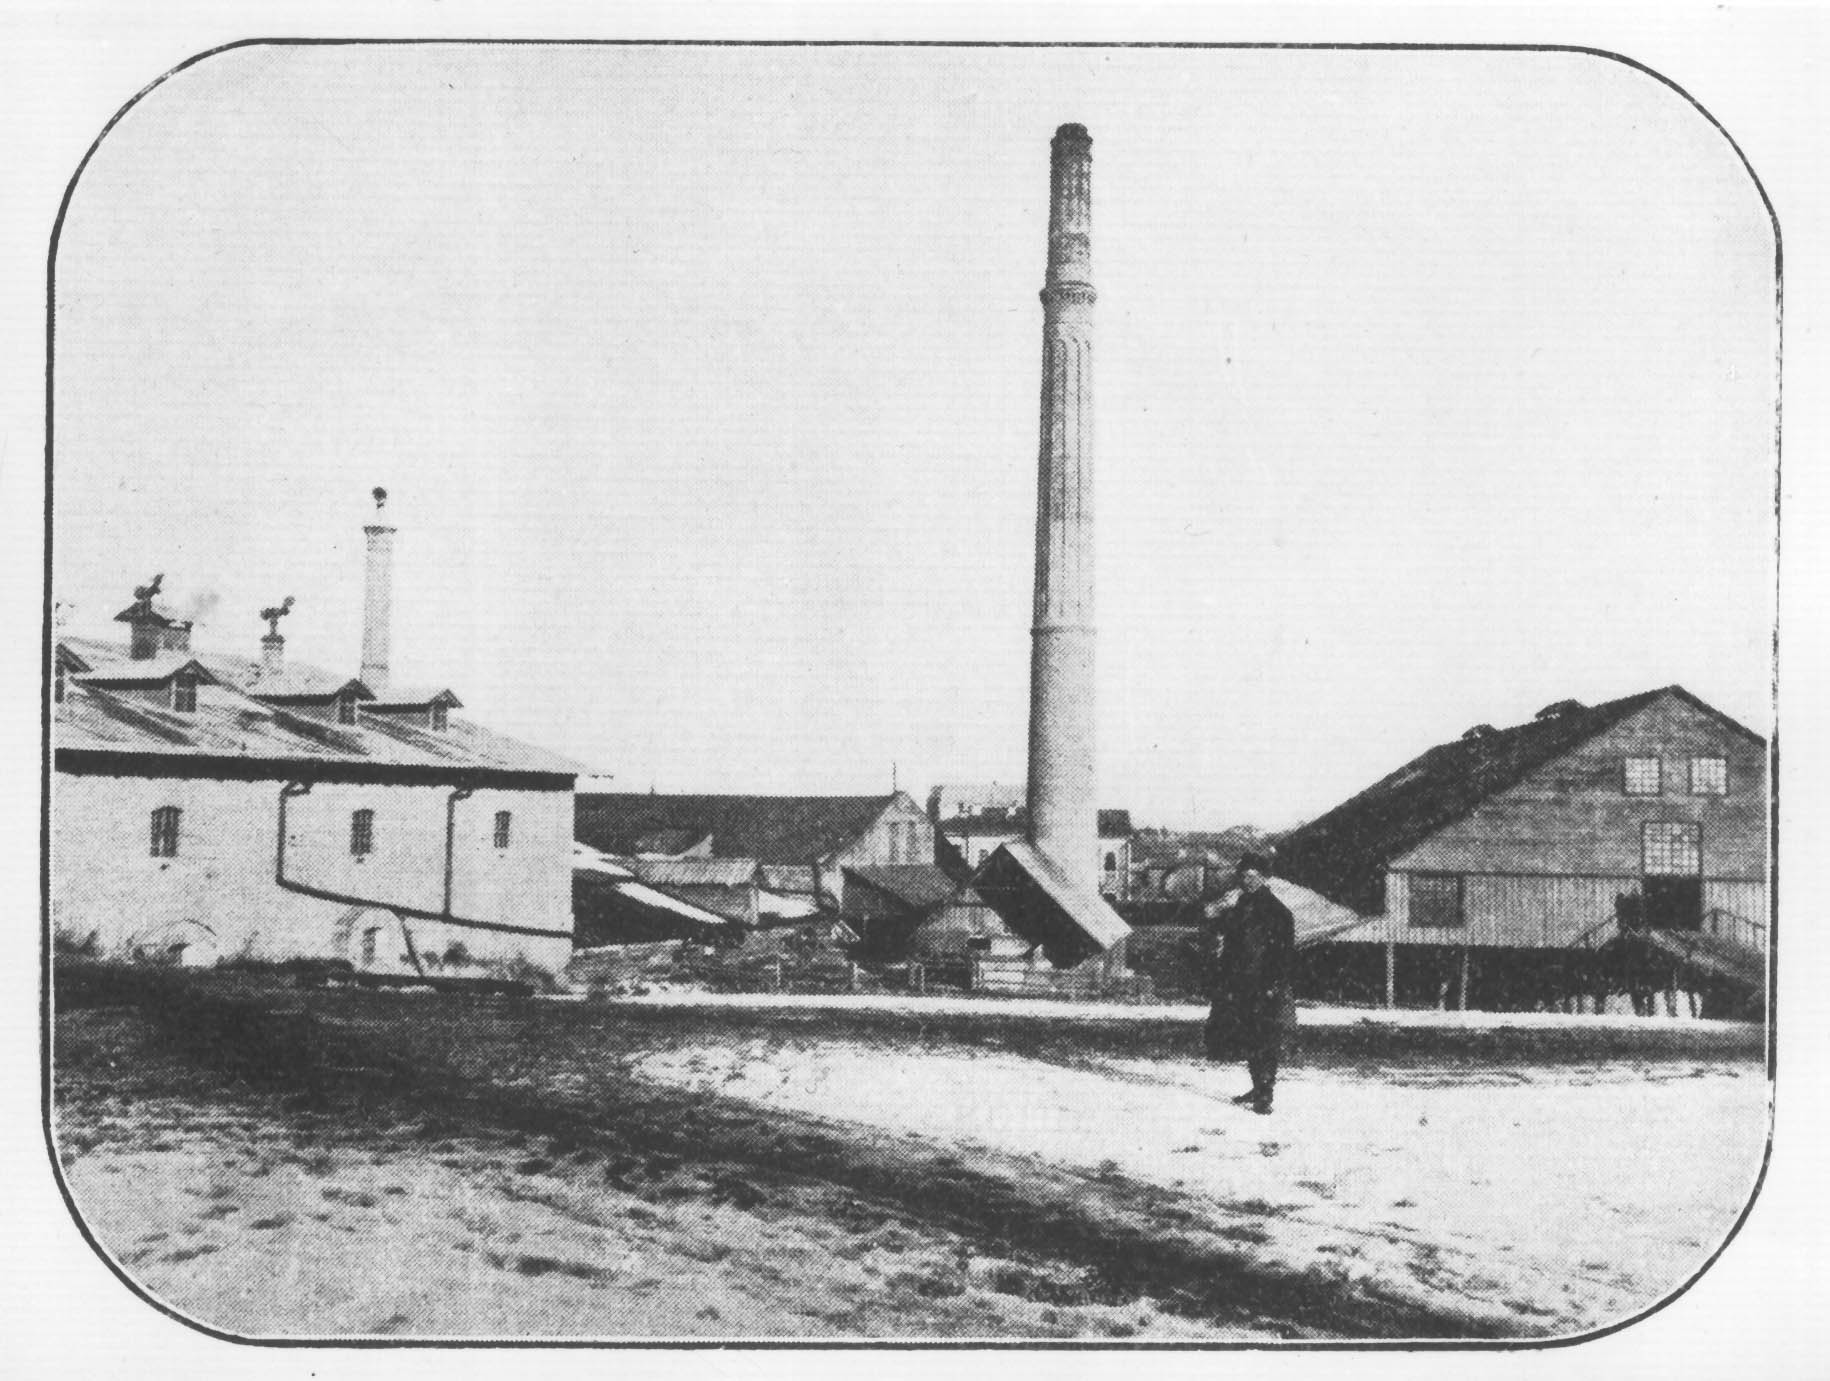
\includegraphics[width=\linewidth]{pix/1897-rihert-kirp.jpg}

\textit{1897. Завод Рихерта.}
\end{center} 
\vspace*{\fill}
\newpage
\vspace*{\fill}
\begin{center}
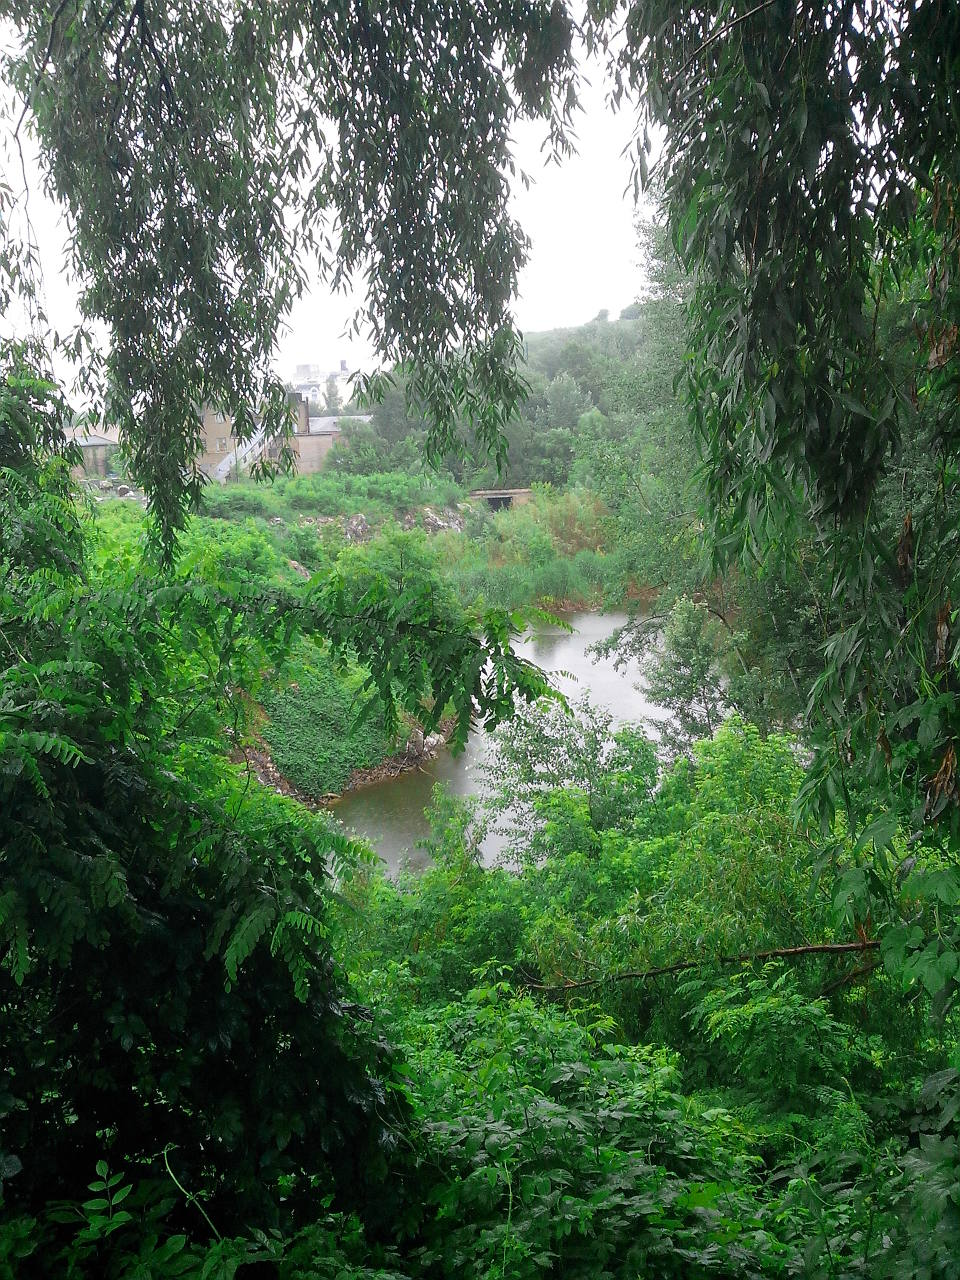
\includegraphics[width=\linewidth]{pix/s-rihert-IMG_20130602_161845.jpg}

\textit{2013. Карьерное озеро за бывшим заводом Рихерта.}
\end{center} 
\vspace*{\fill}
\newpage

\begin{center}
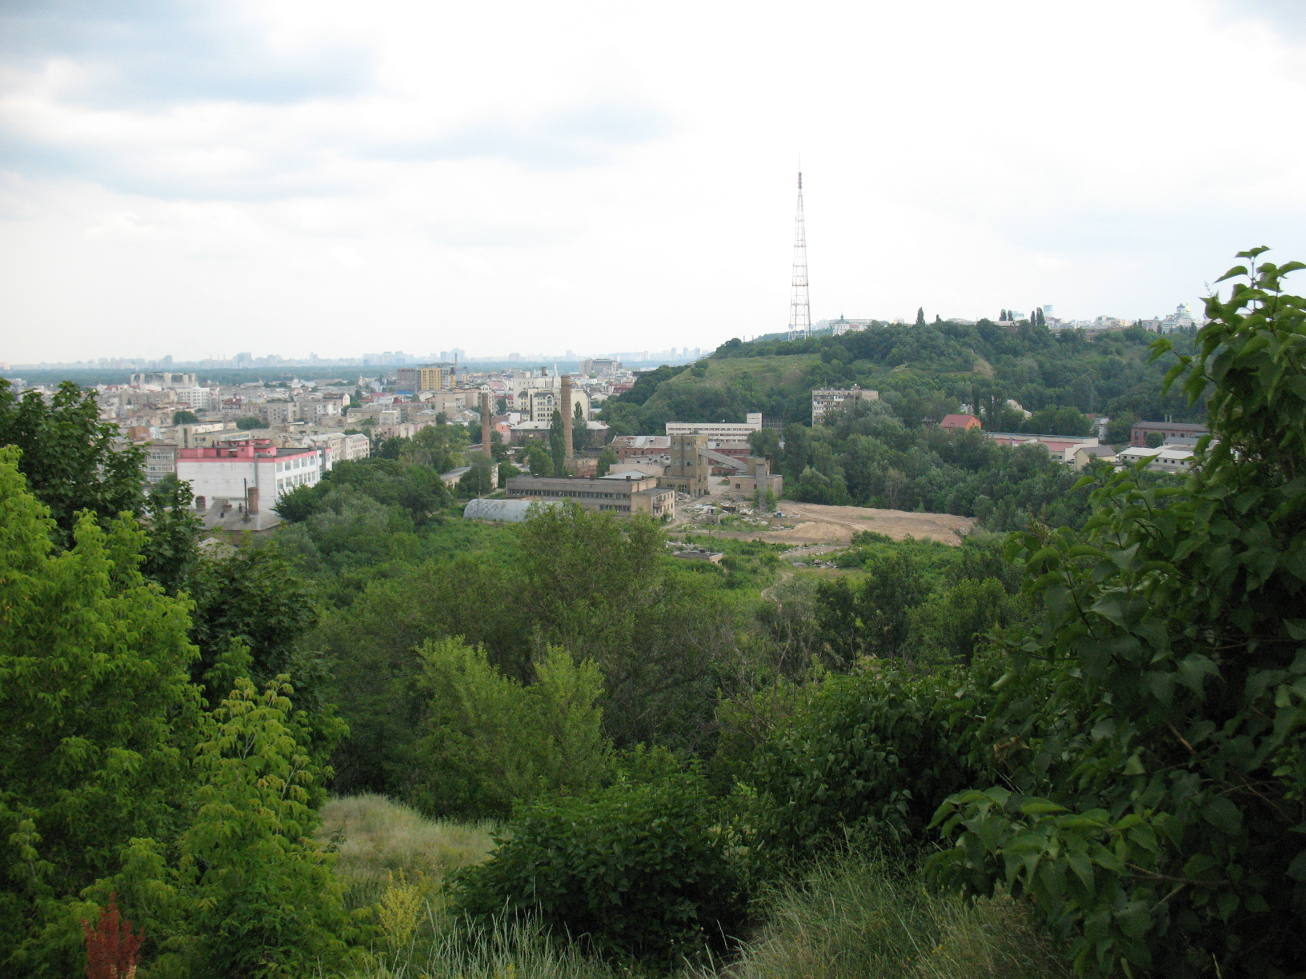
\includegraphics[width=0.98\linewidth]{pix/s-rihert-IMG_4358.JPG}

\textit{2015. Вид на бывший завод Рихерта с севера. На месте грязи раньше был склон Лысой горы.}
\end{center} 

\begin{center}
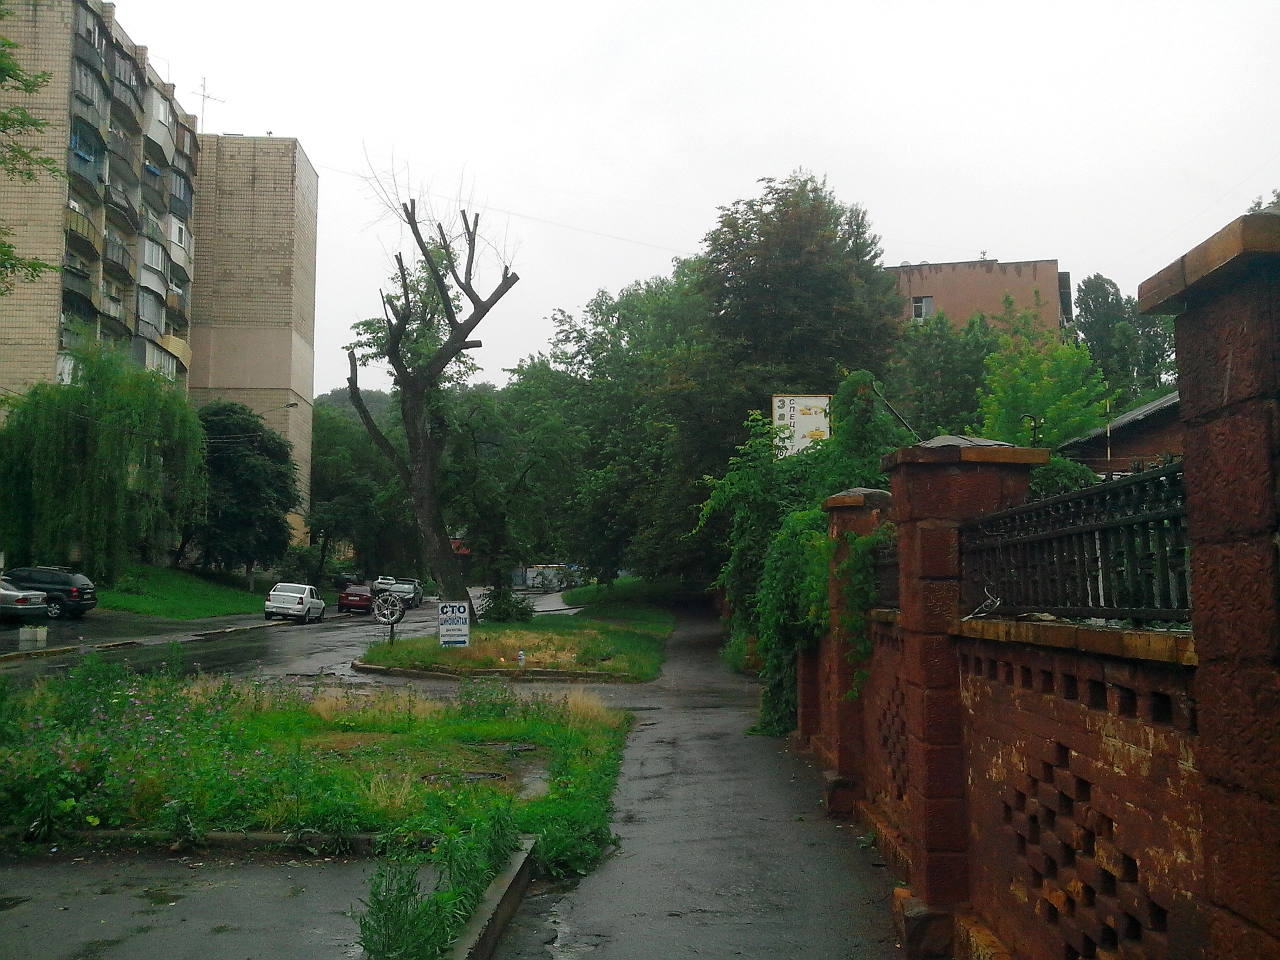
\includegraphics[width=0.98\linewidth]{pix/s-rihert-IMG_20130602_163103.jpg}

\textit{2013. Заводской забор на Нижнеюрковской, 2.}
\end{center} 

\newpage

\begin{center}
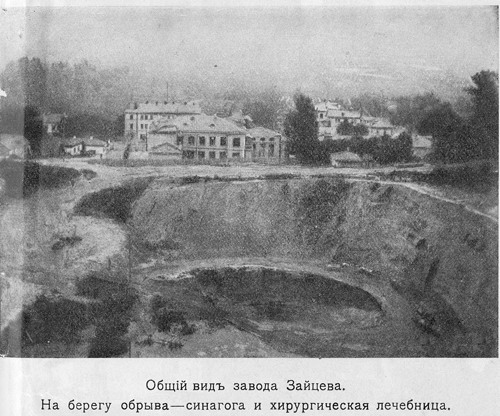
\includegraphics[width=\linewidth]{pix/zavod-zaiceva.png}
\end{center} 

\begin{center}
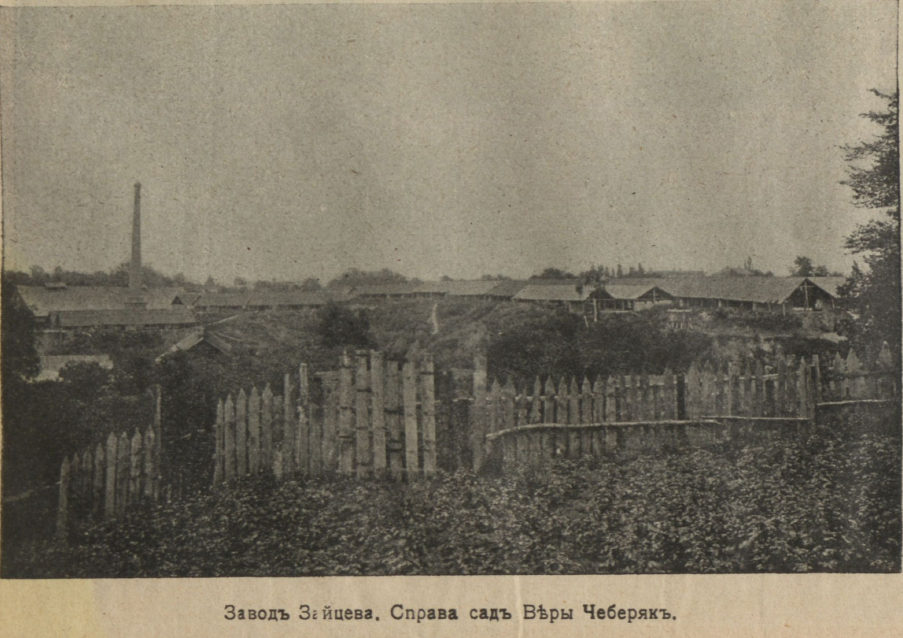
\includegraphics[width=\linewidth]{pix/1912-beylis-03.jpg}
\end{center} 

\newpage
\vspace*{\fill}
\begin{center}
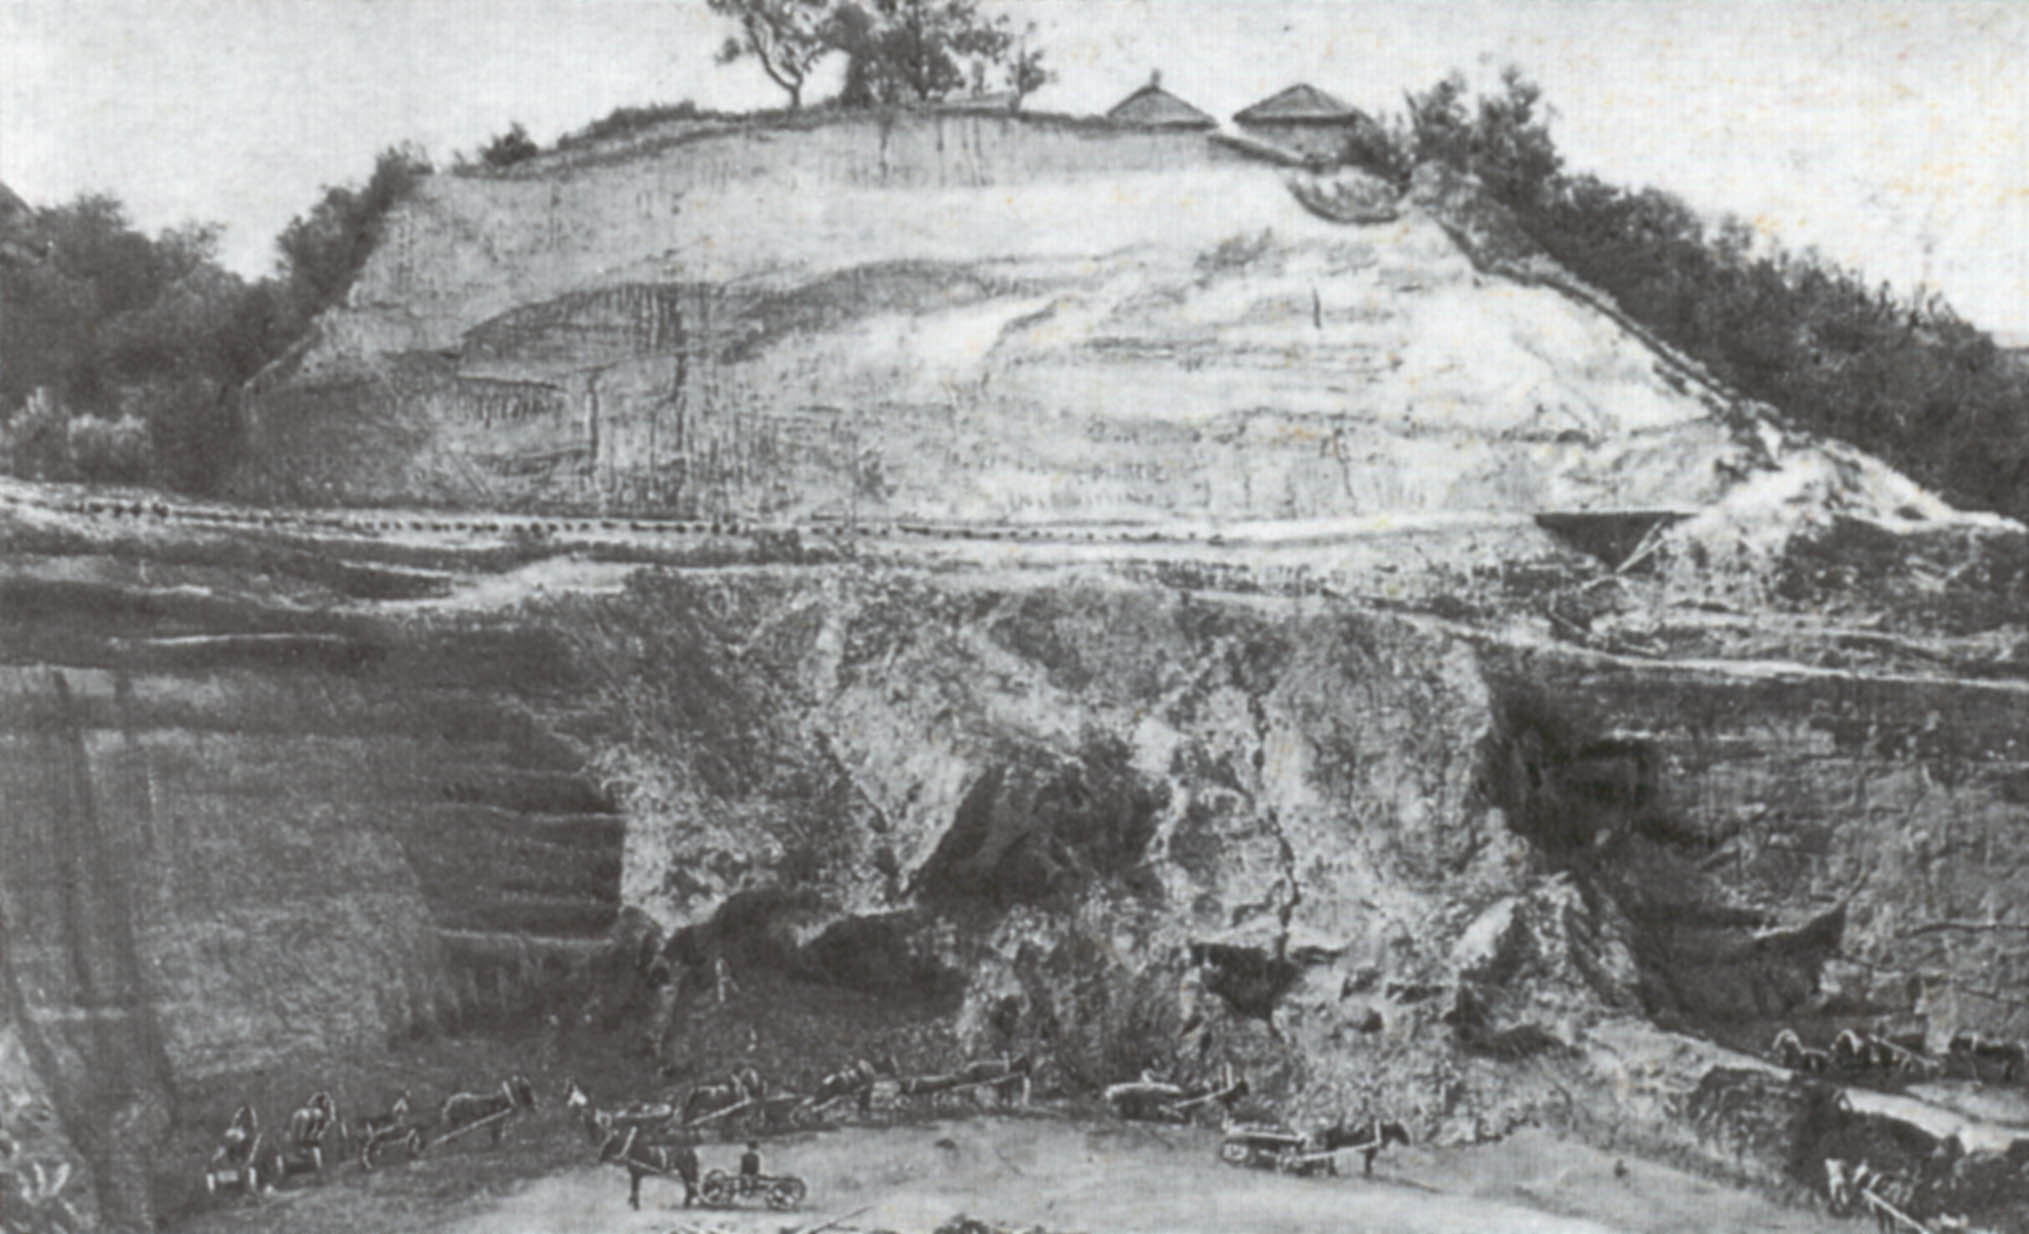
\includegraphics[width=\linewidth]{pix/hvoyka-02.jpg}

\textit{Глинище завода Зайцева во время раскопок Кирилловской стоянки.}
\end{center} 

\begin{center}
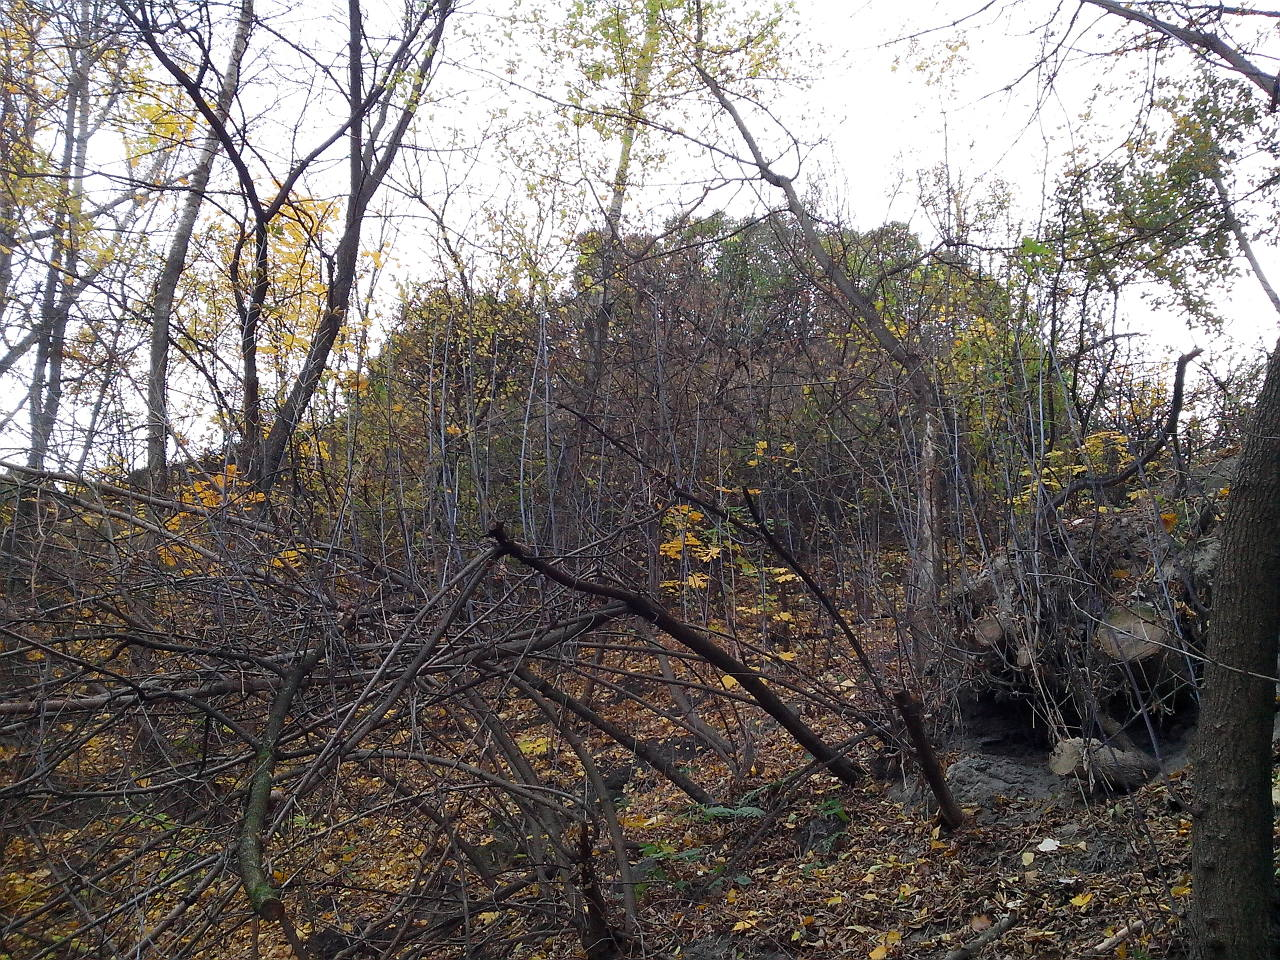
\includegraphics[width=\linewidth]{pix/s-IMG_20131020_163317.jpg}

\textit{2013. Остатки склона над глинищем.}
\end{center} 
\vspace*{\fill}
\newpage
\vspace*{\fill}
\begin{center}
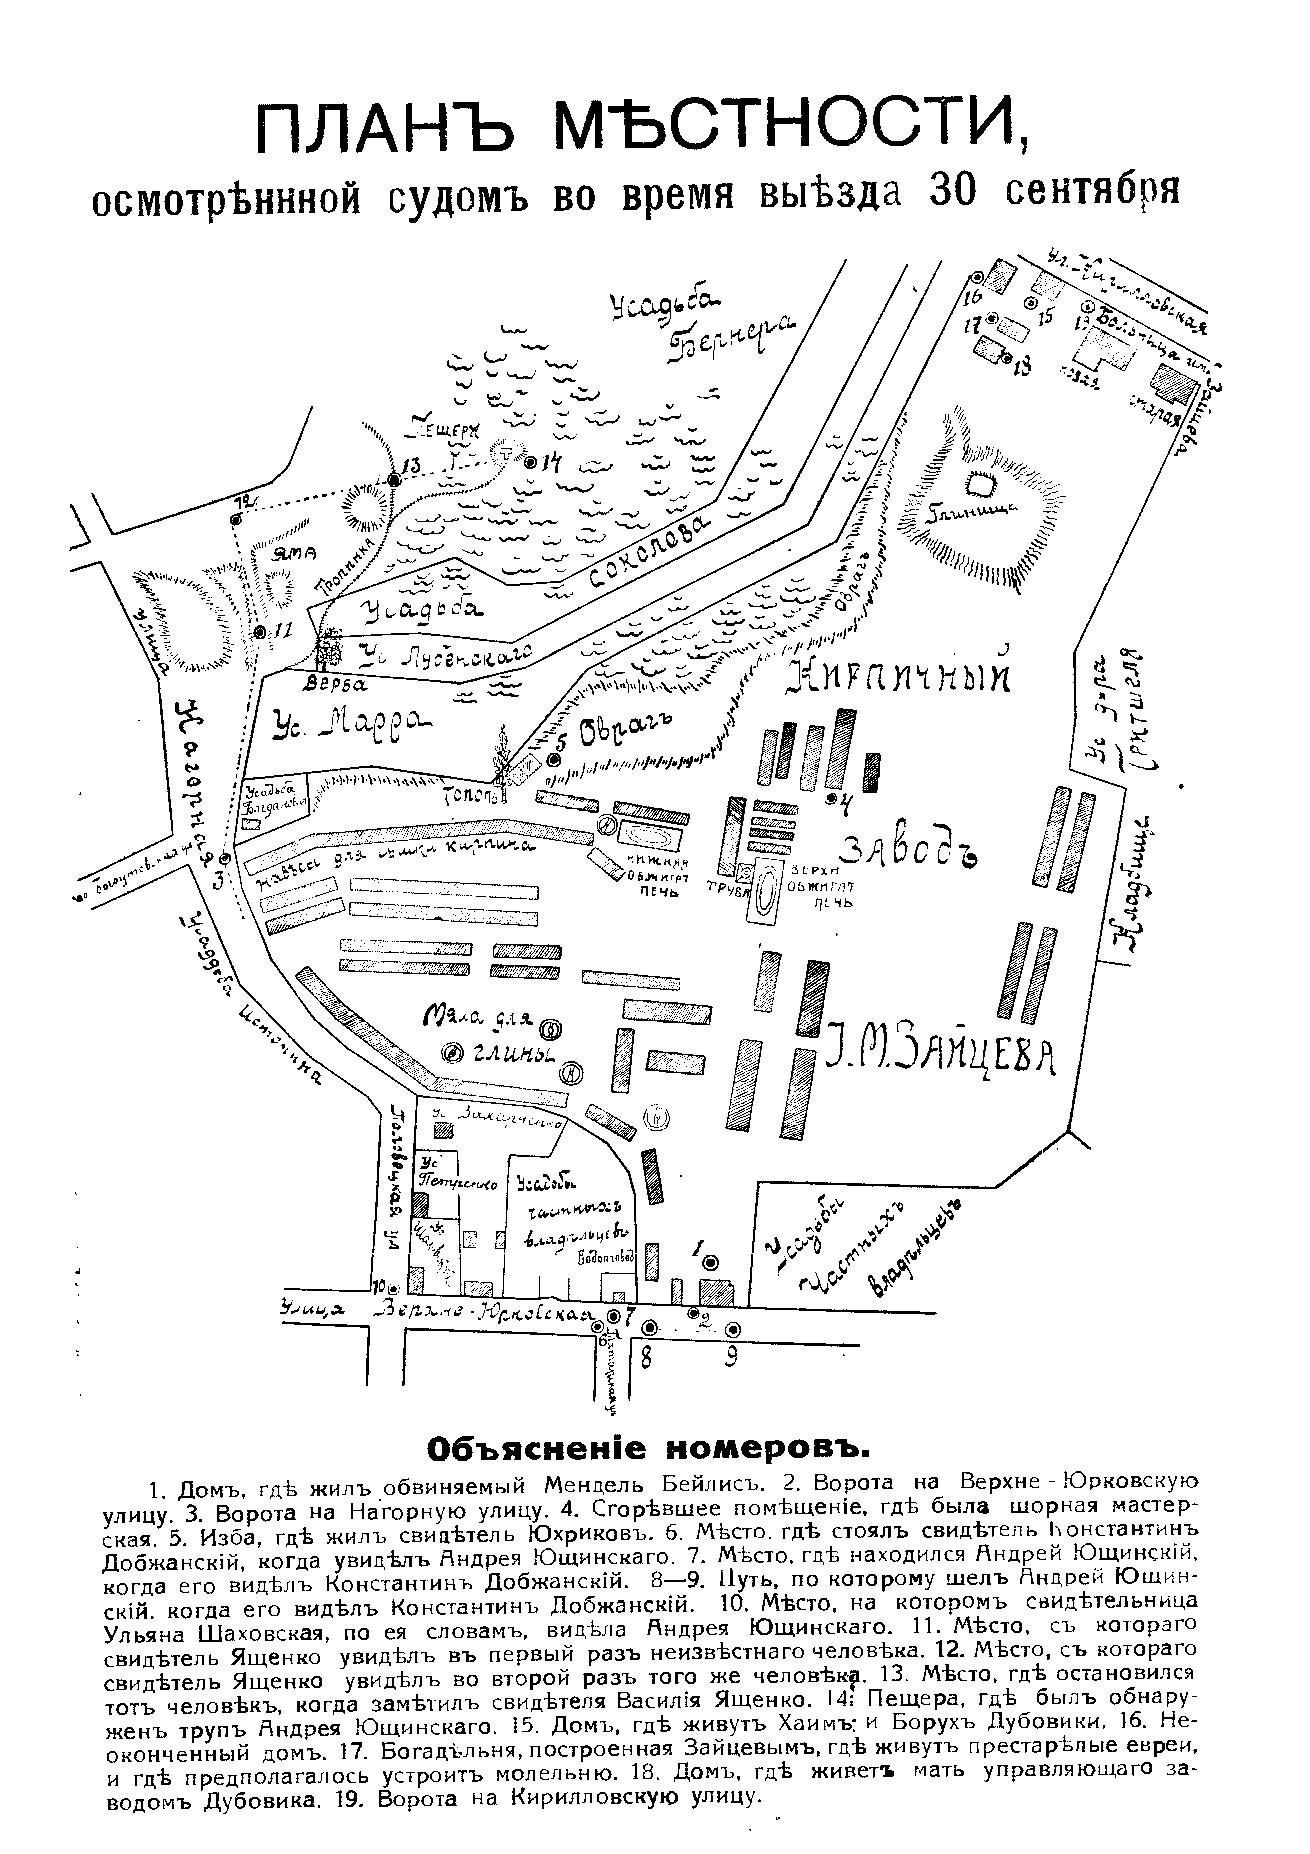
\includegraphics[width=\linewidth]{pix/1913-karta.jpg}

\textit{1913, карта из материалов дела Бейлиса.}
\end{center} 
\vspace*{\fill}
\newpage
\vspace*{\fill}
\begin{center}
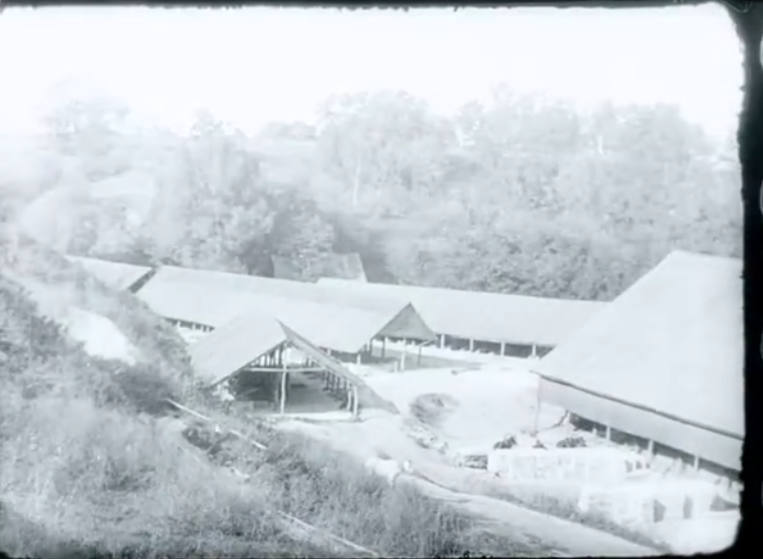
\includegraphics[width=\linewidth]{pix/zaic.jpg}
\end{center} 

\begin{center}
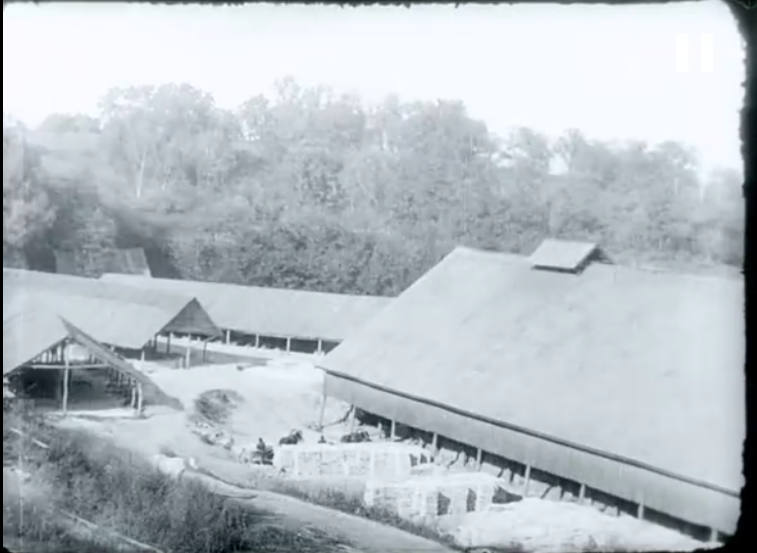
\includegraphics[width=\linewidth]{pix/zaic02.jpg}
\textit{1912. Кирпичный завод Зайцева вблизи.}
\end{center} 
\vspace*{\fill}
\newpage
\vspace*{\fill}
\begin{center}
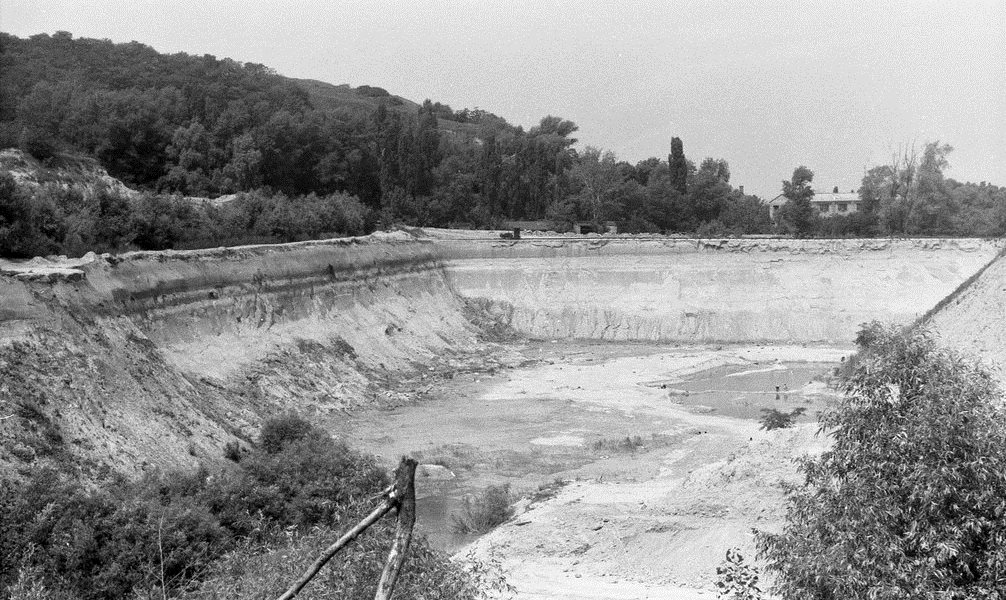
\includegraphics[width=\linewidth]{pix/syrec-06.jpg}

\textit{1950-60, один из карьеров Петровских кирпичных заводов в пойме речки Сырец.}
\end{center} 


\begin{center}
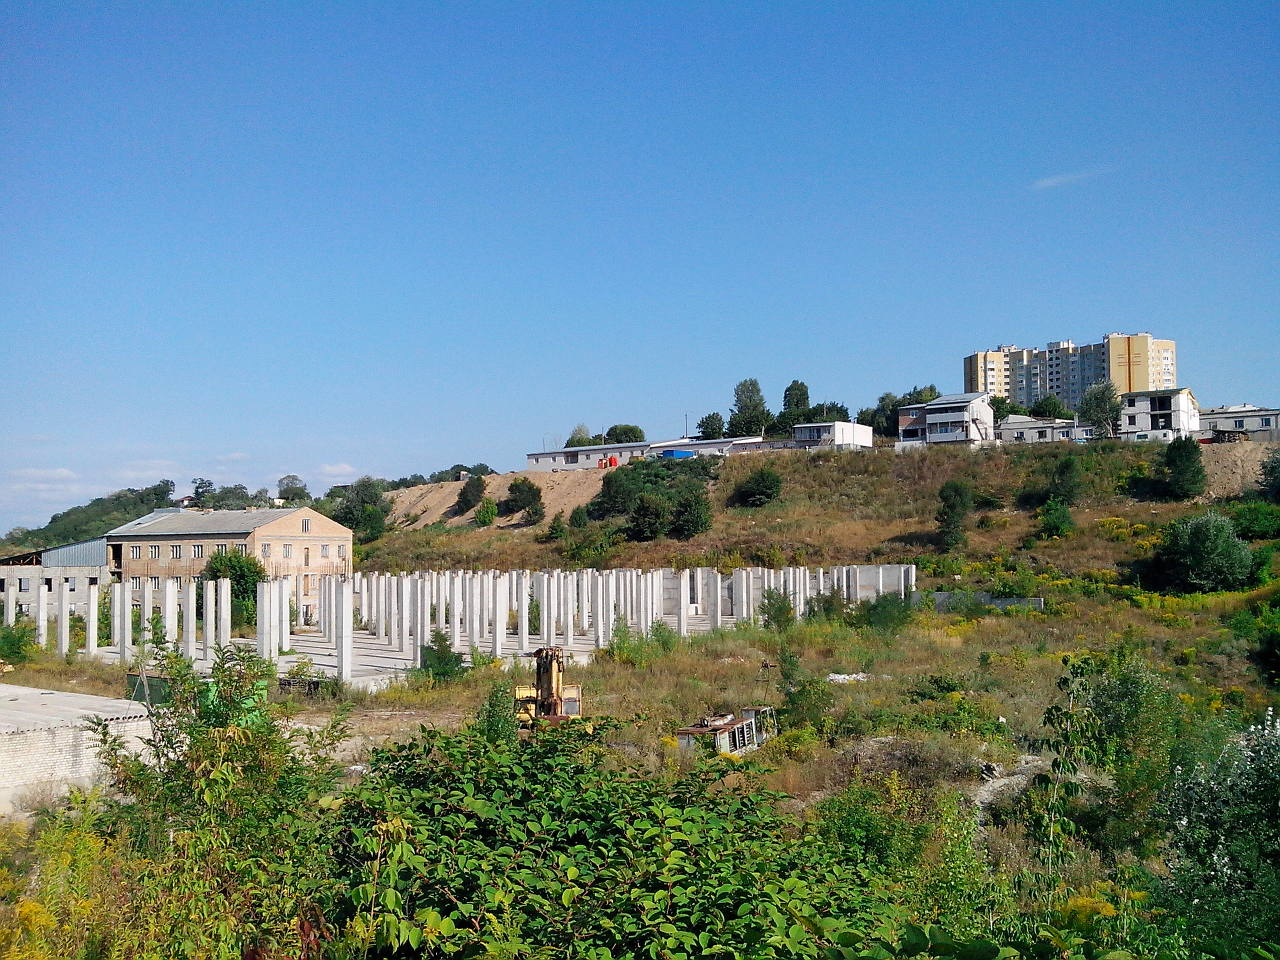
\includegraphics[width=\linewidth]{pix/s-syrec-IMG_20130812_163717.jpg}

\textit{2013, склоны глинища Петровских заводов за Сырецкой, 33Ш.}
\end{center} 
\vspace*{\fill}
\newpage

\begin{center}
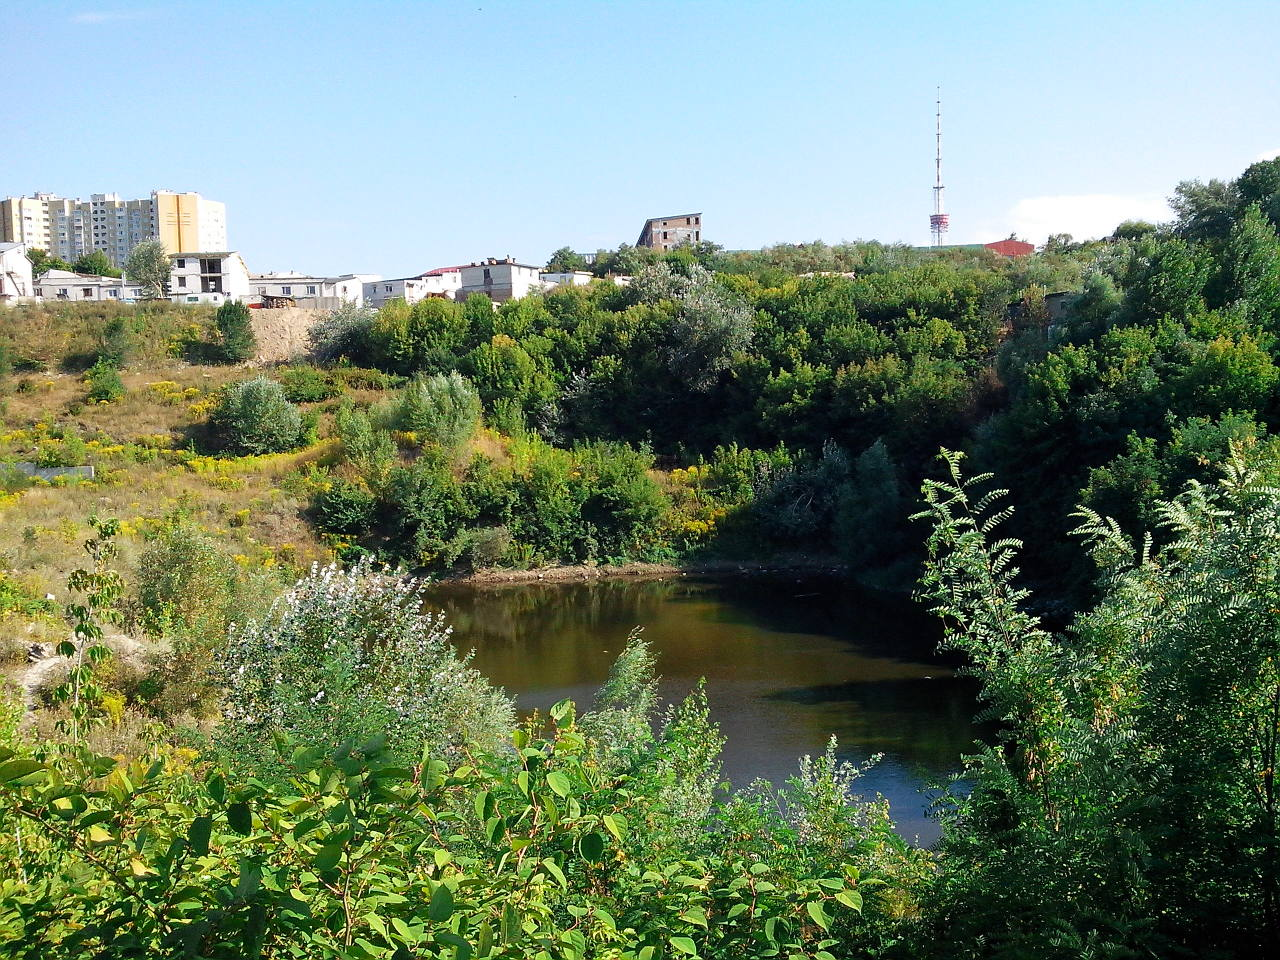
\includegraphics[width=\linewidth]{pix/s-syrec-IMG_20130812_163712.jpg}

\textit{2013, там же, карьерное озеро.}
\end{center} 

\begin{center}
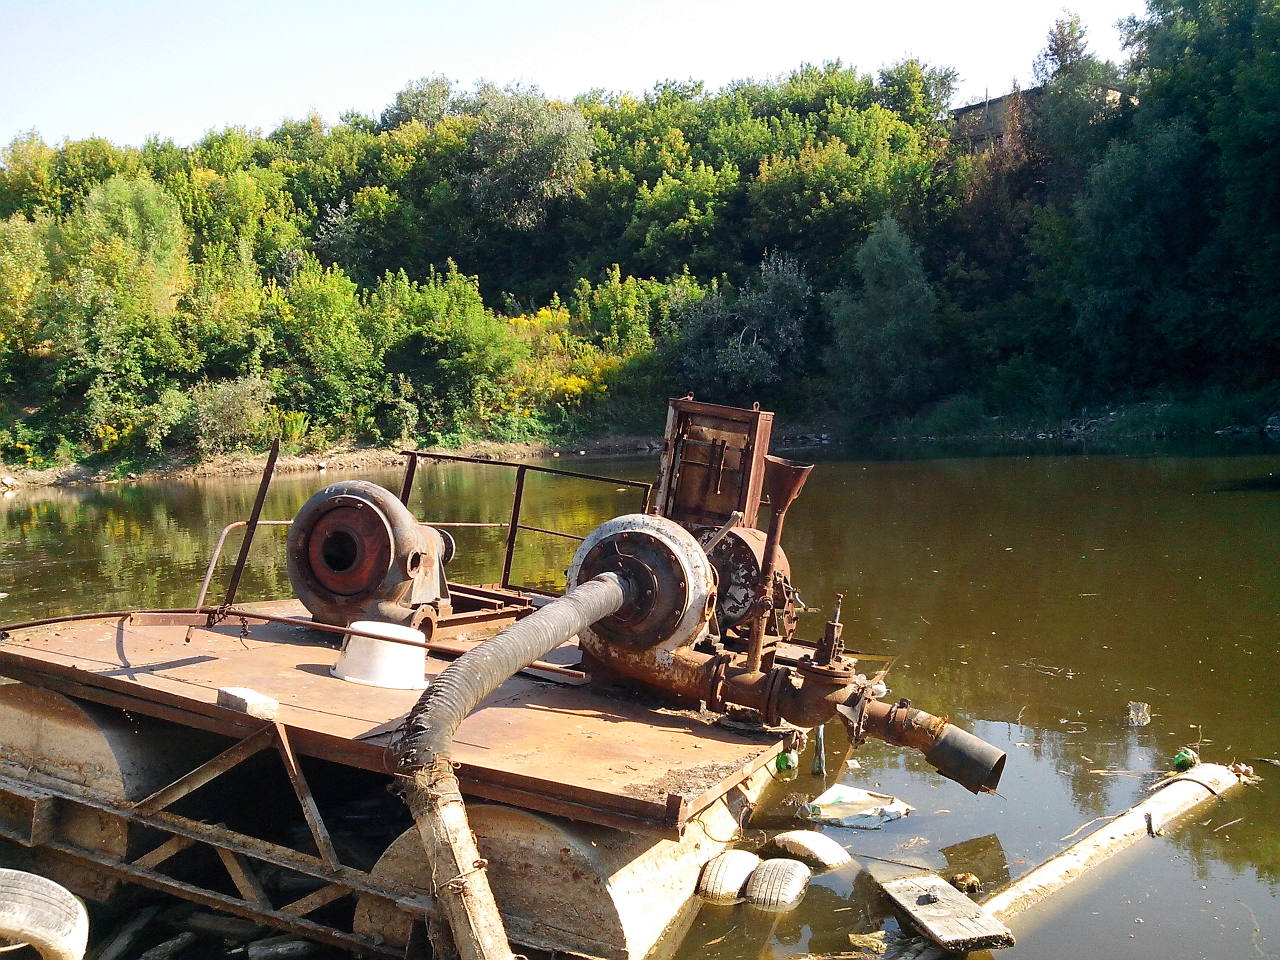
\includegraphics[width=\linewidth]{pix/s-syrec-IMG_20130812_164051.jpg}

\textit{2013, там же.}
\end{center} 

\newpage
\vspace*{\fill}
\begin{center}
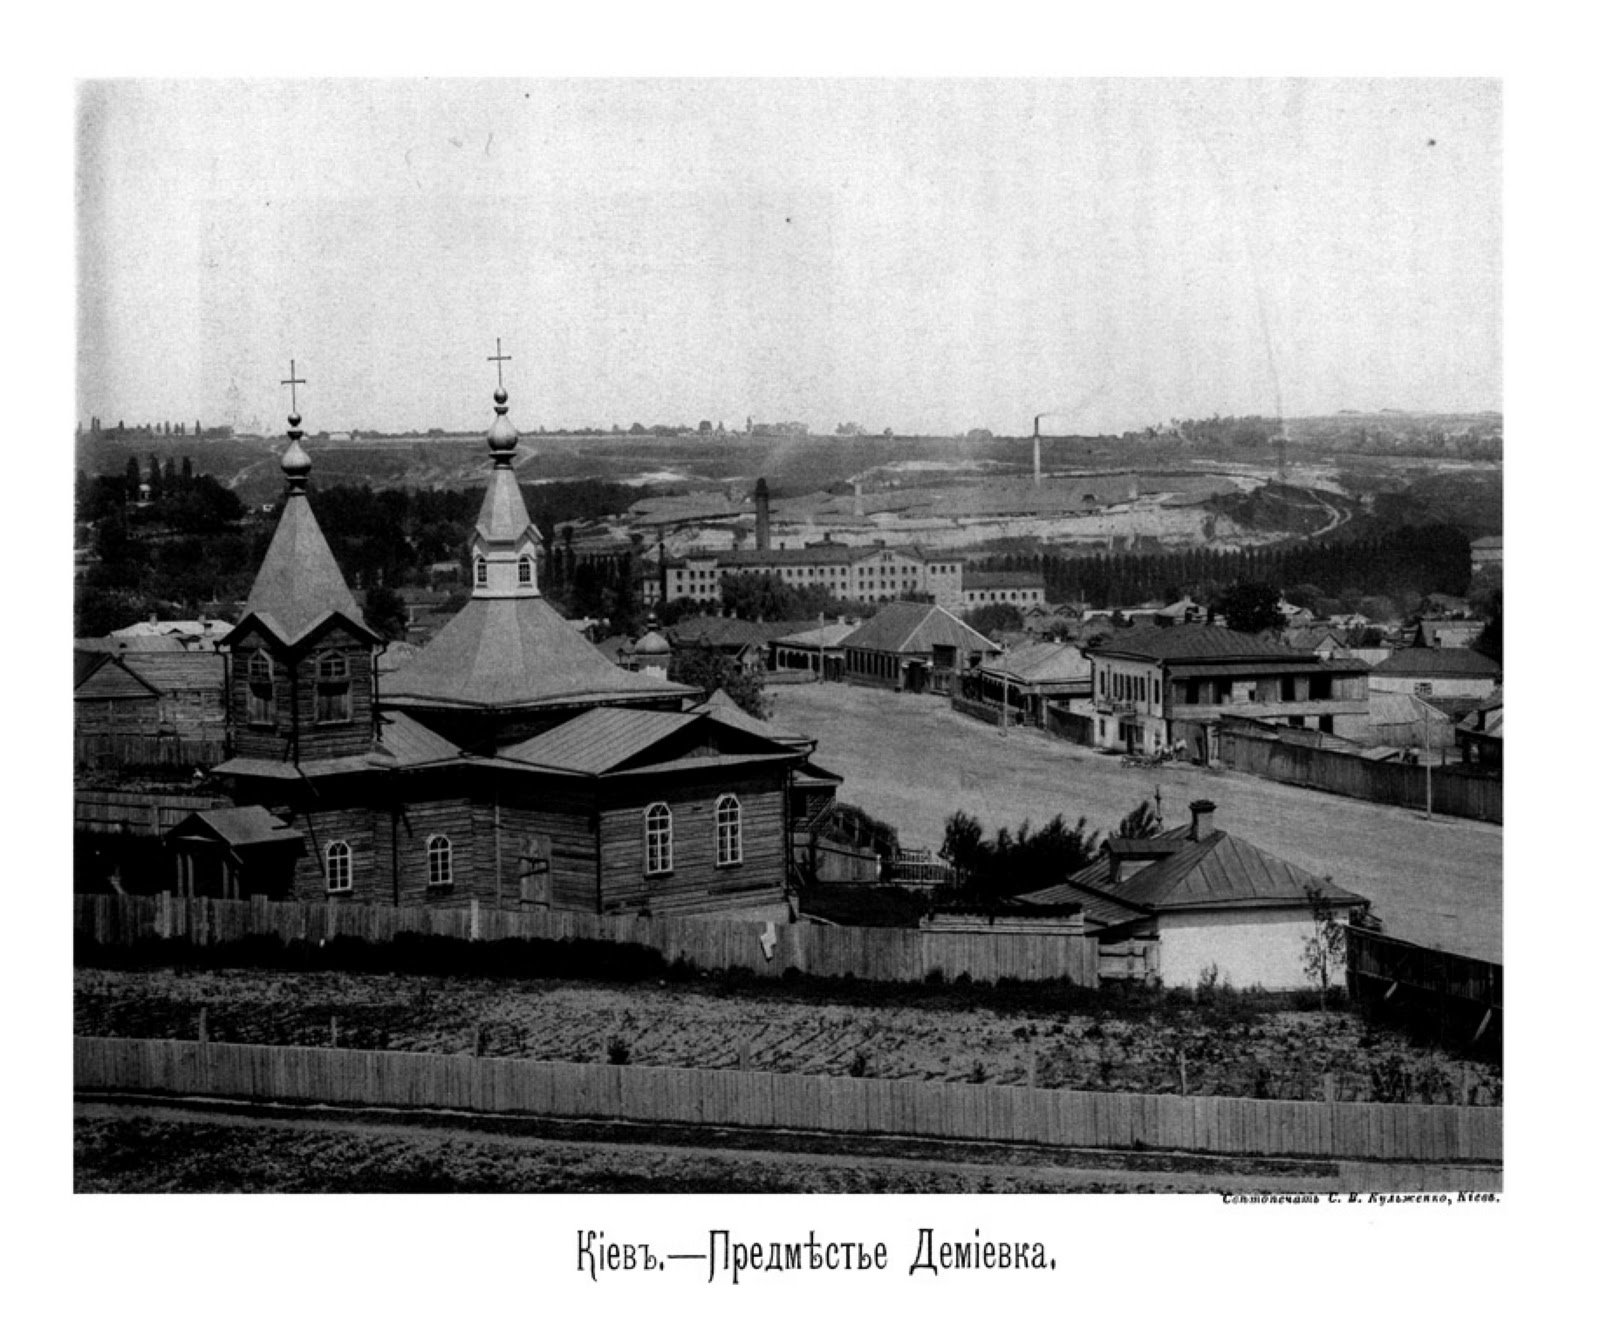
\includegraphics[width=\linewidth]{pix/24.jpeg}
\end{center} 

\textit{1888 год, фото из книги М. Захарченко «Киев теперь и прежде». Ближайшая труба на заднем плане – сахарорафинадного завода (в советское время там расположилась кондитерская фабрика имени Карла Маркса), а вот за ним – трубы заводов Субботиной и Шатовой, и глинища оных. Слева – Вознесенская церковь, стоит и поныне, на Голосеевском проспекте.}
\vspace*{\fill}
\newpage
\vspace*{\fill}
\begin{center}
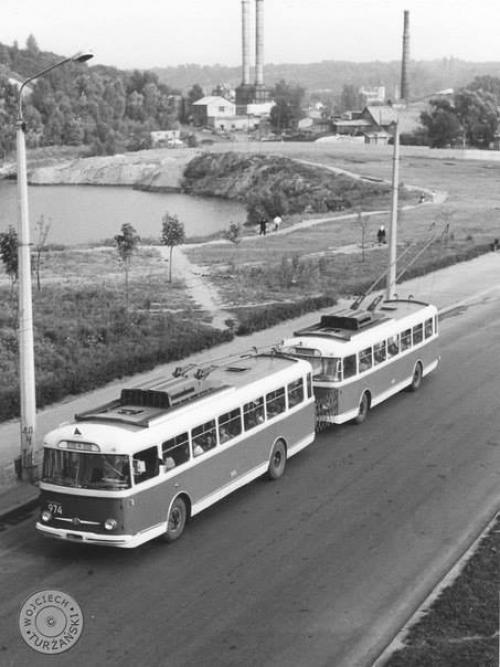
\includegraphics[width=\linewidth]{pix/woitech.jpg}
\end{center} 

\textit{После 1966 года, озеро Глинка (частично по месту глинища Субботиной), на заднем плане – трубы кирпичного завода. Фото Wojtiech Turzanski.}
\vspace*{\fill}
\newpage

\begin{center}
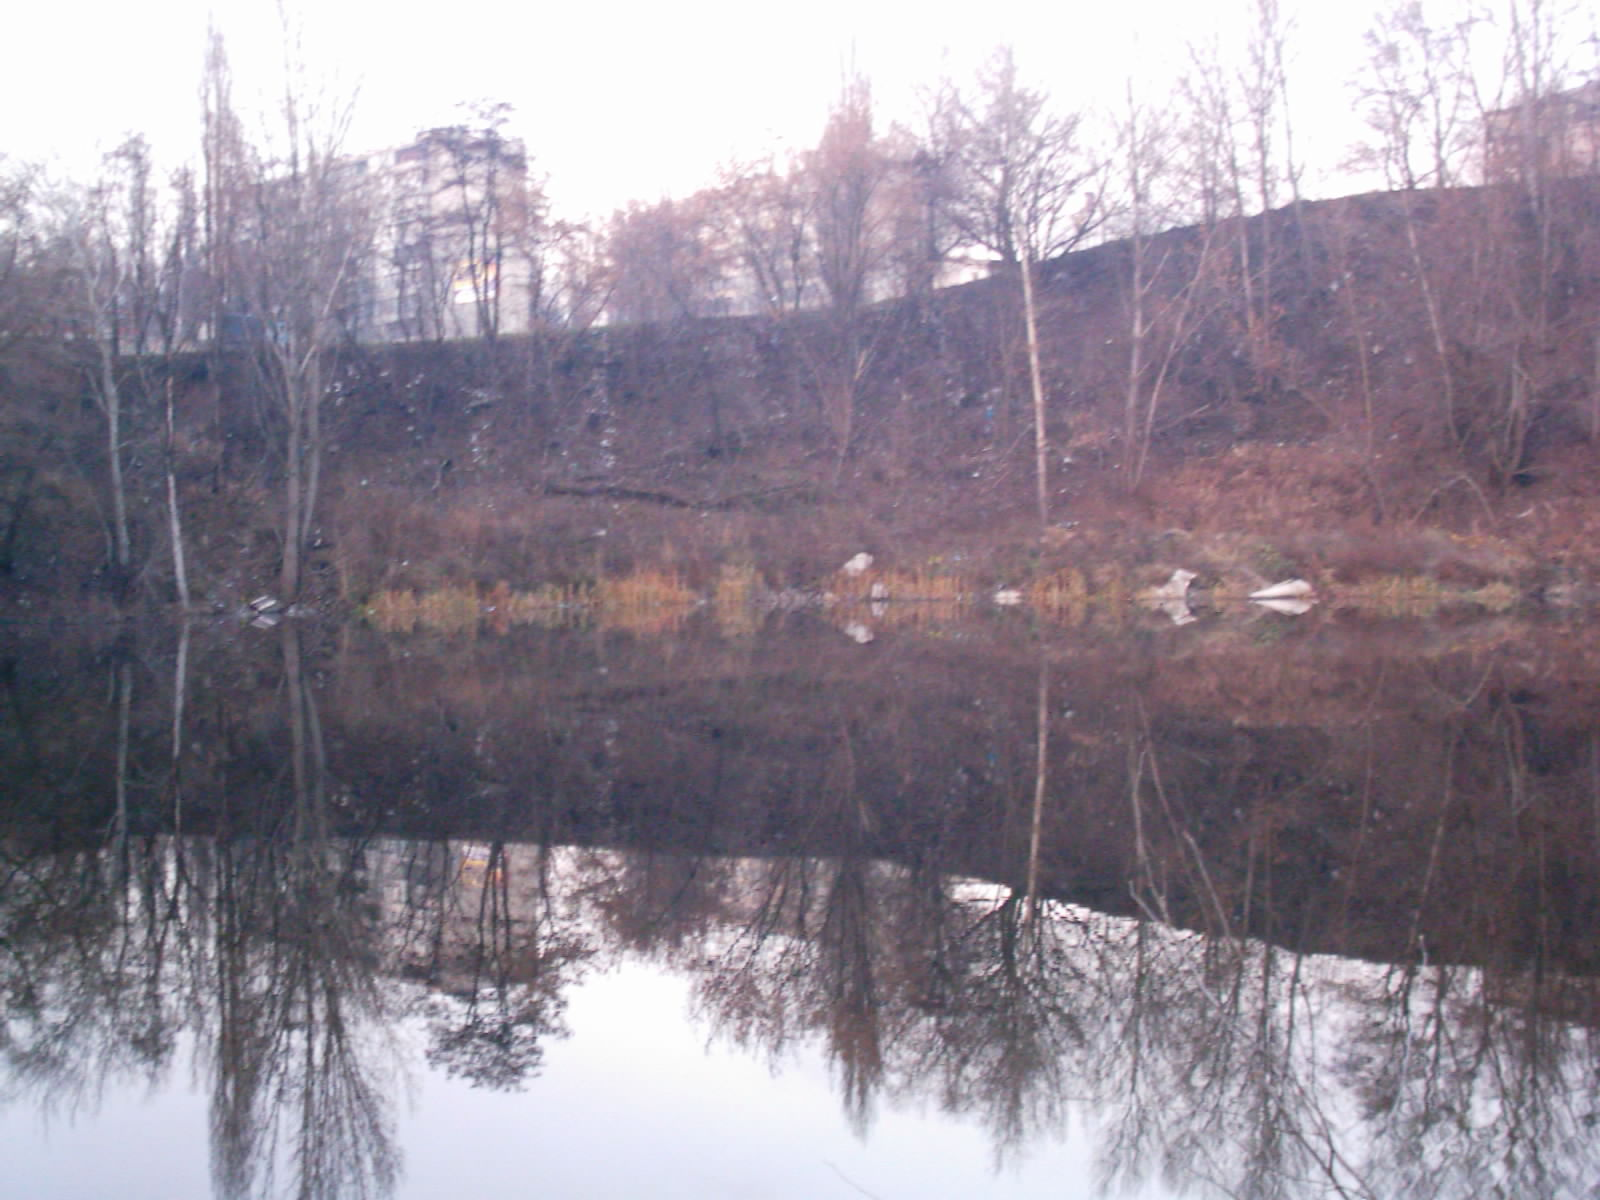
\includegraphics[width=\linewidth]{pix/glinka-imag0022.jpg}
\textit{2005, озеро Глинка.}
\end{center} 

\begin{center}
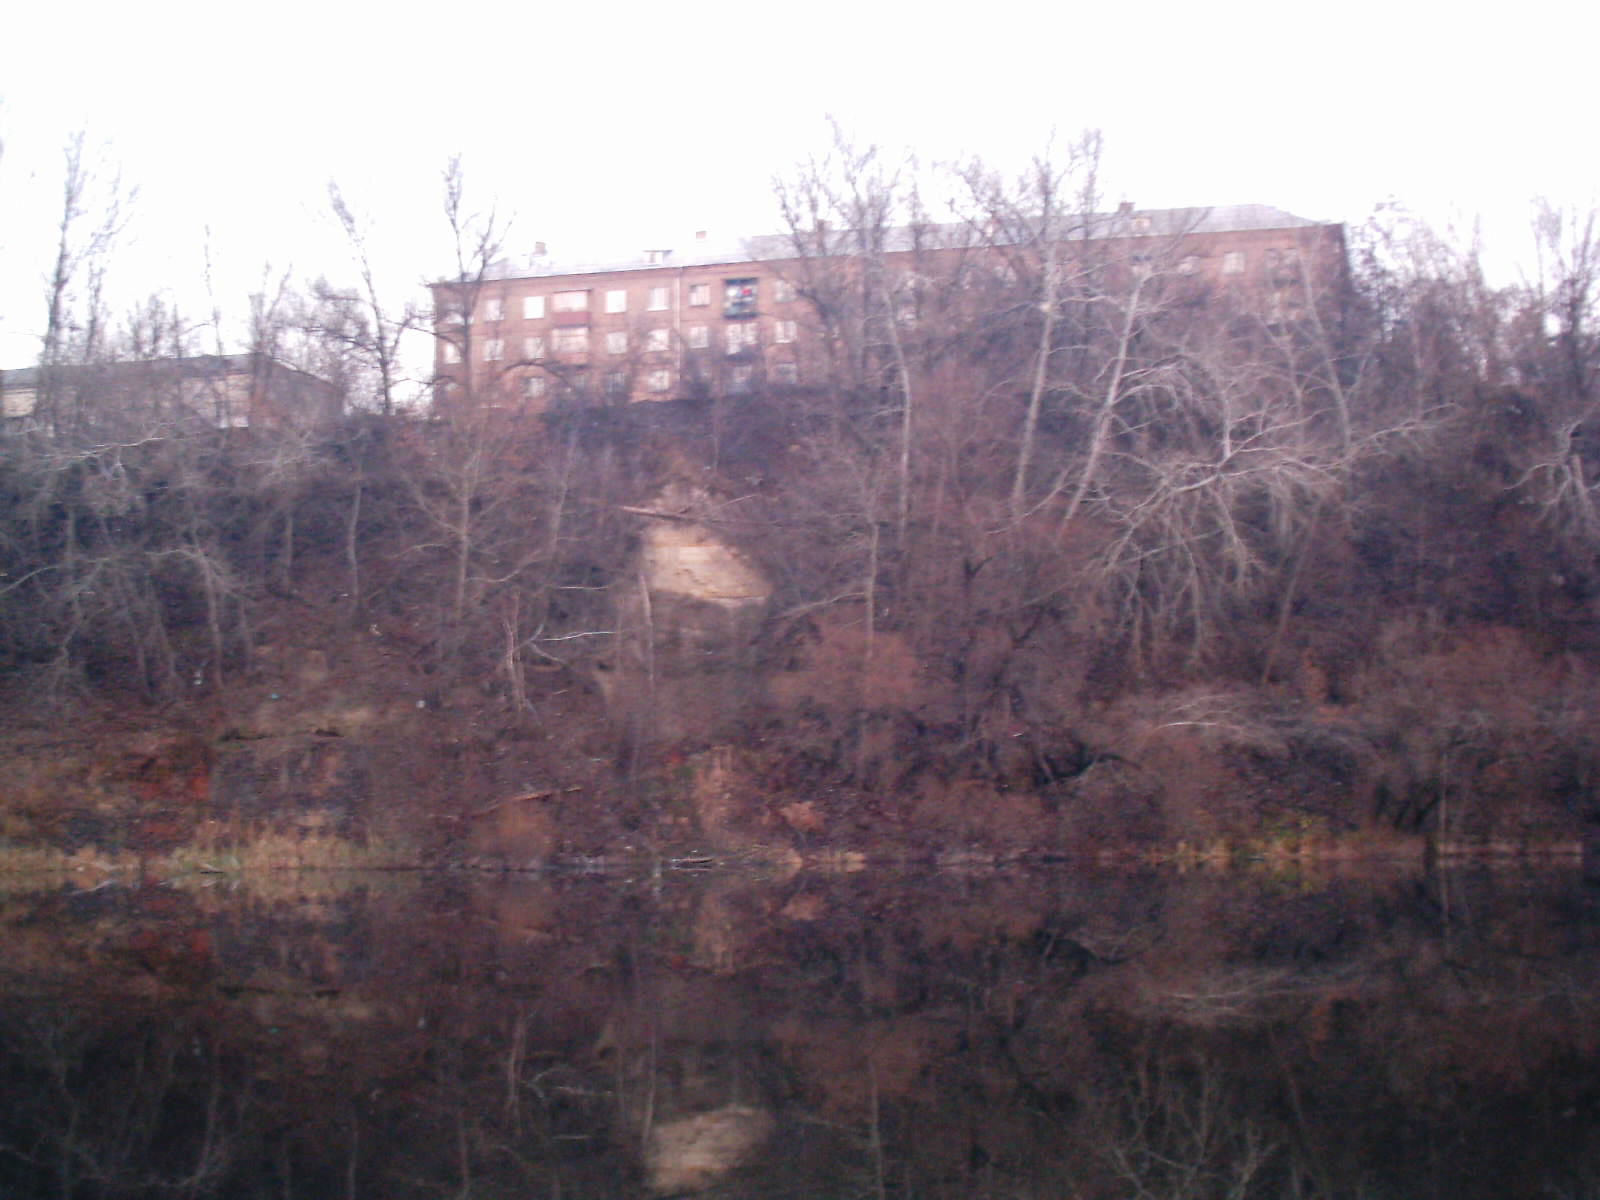
\includegraphics[width=\linewidth]{pix/glinka-imag0018.jpg}

\textit{2005, озеро Глинка.}
\end{center} 
\newpage

\begin{center}
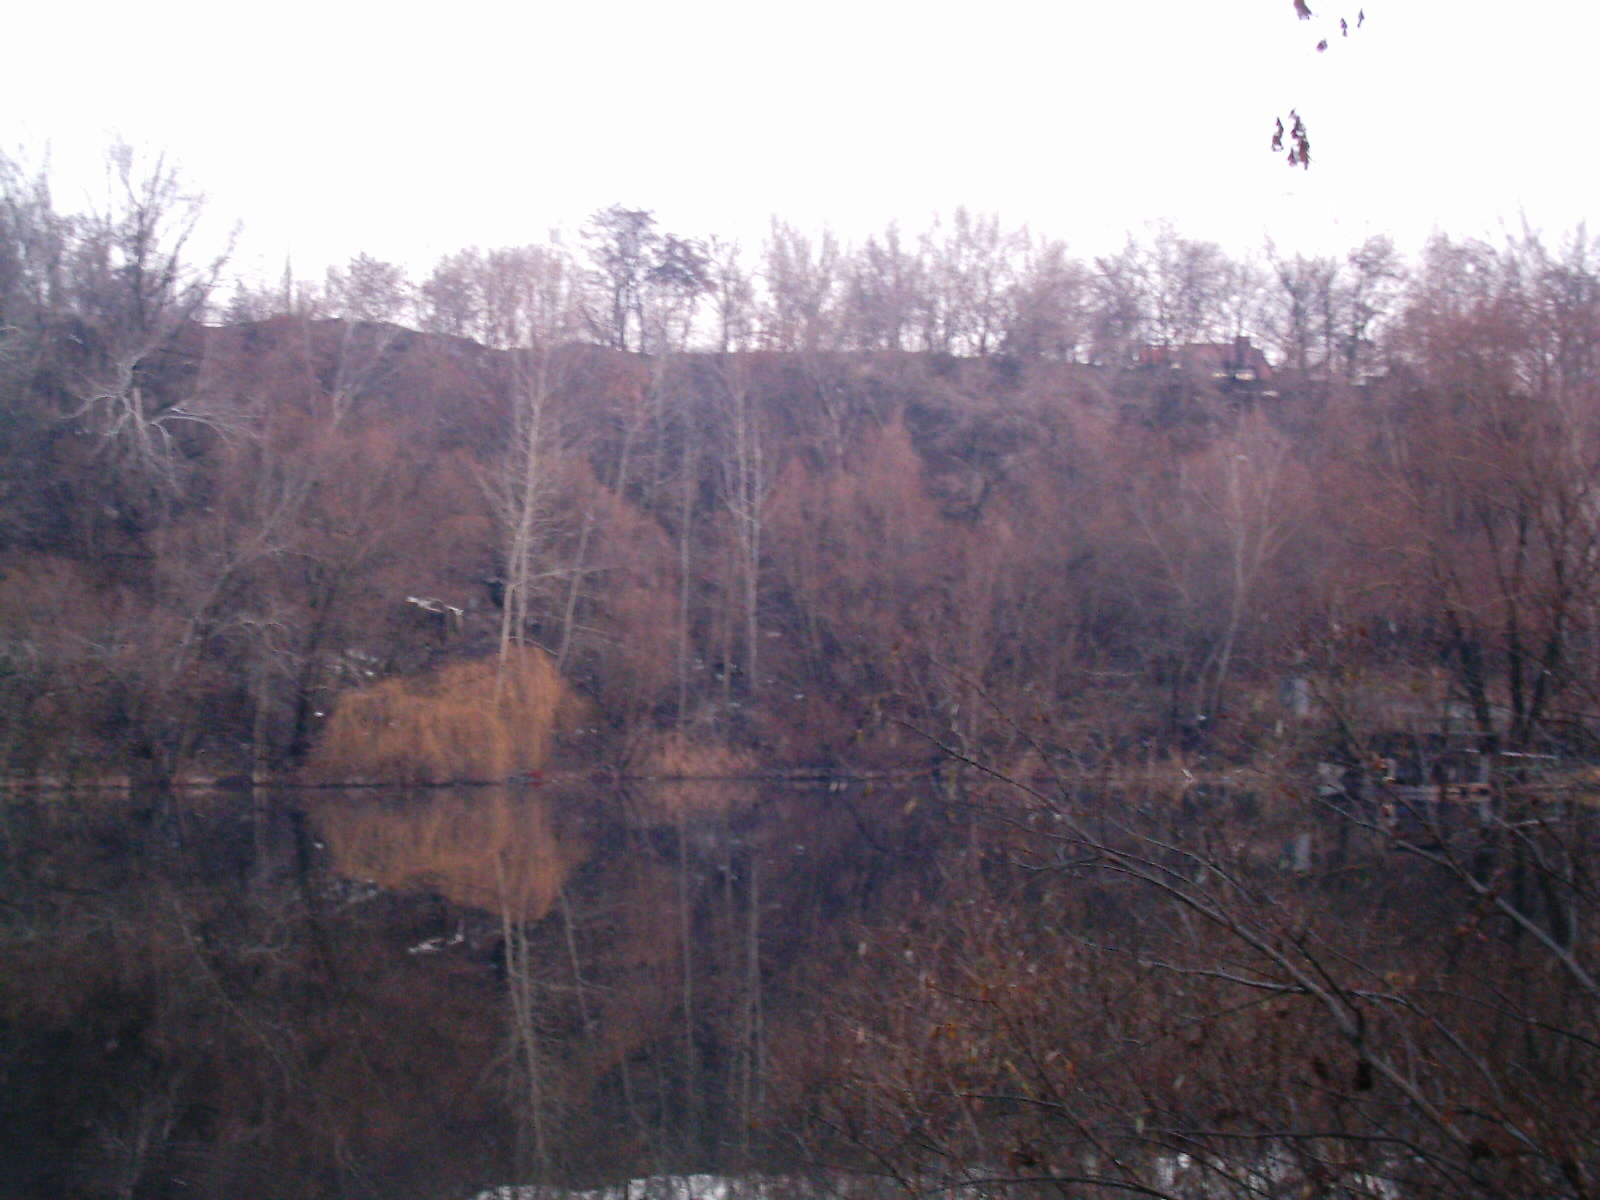
\includegraphics[width=\linewidth]{pix/glinka-imag0019.jpg}
\textit{2005, озеро Глинка.}
\end{center} 

\begin{center}
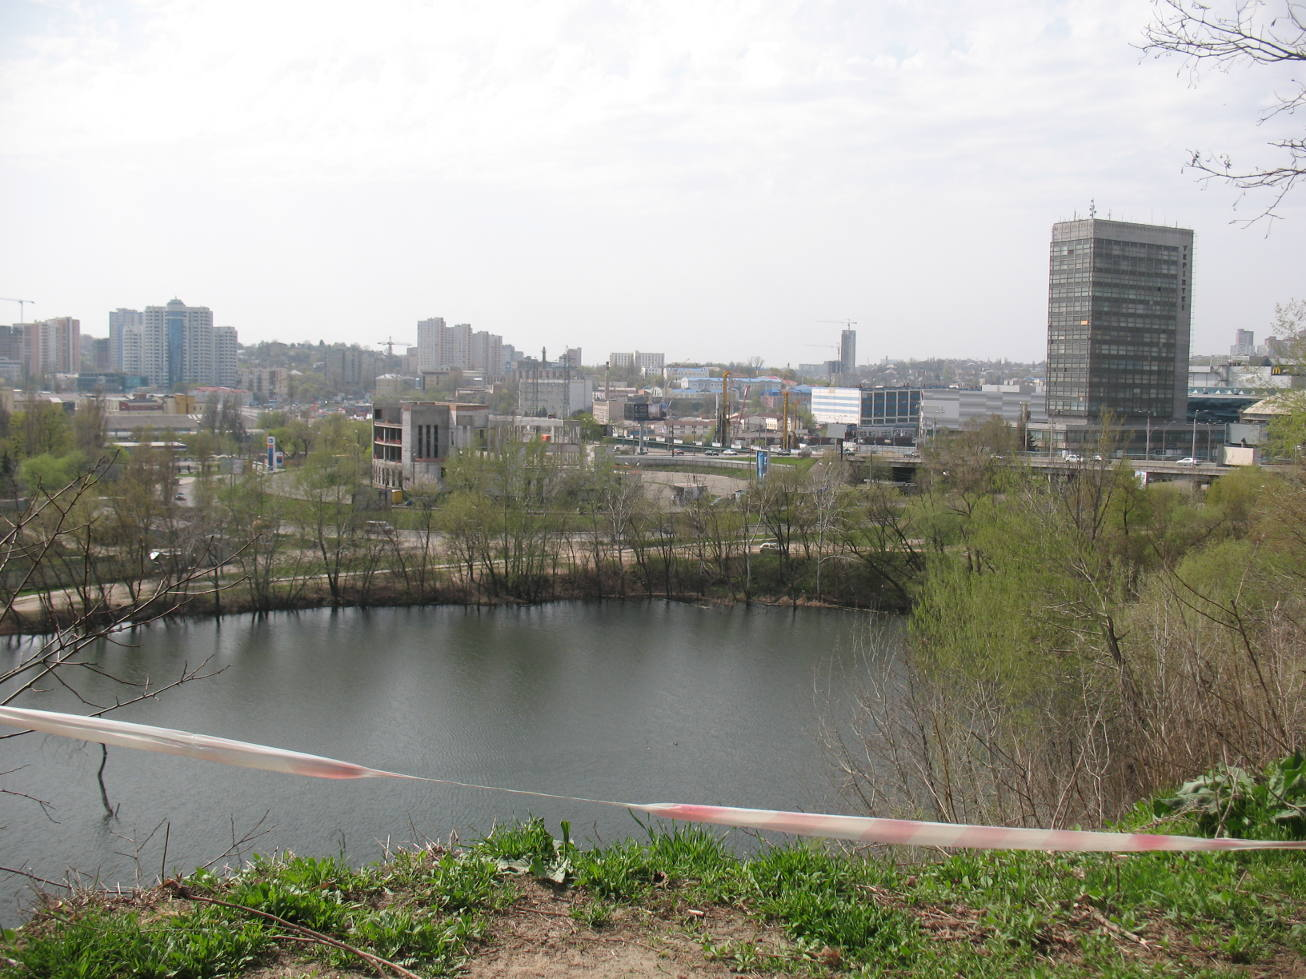
\includegraphics[width=\linewidth]{pix/s-glinka-IMG_4542.JPG}
\textit{2016, озеро Глинка, вид с обрыва. Позади – Демиевка.}
\end{center} 

\newpage

\begin{center}
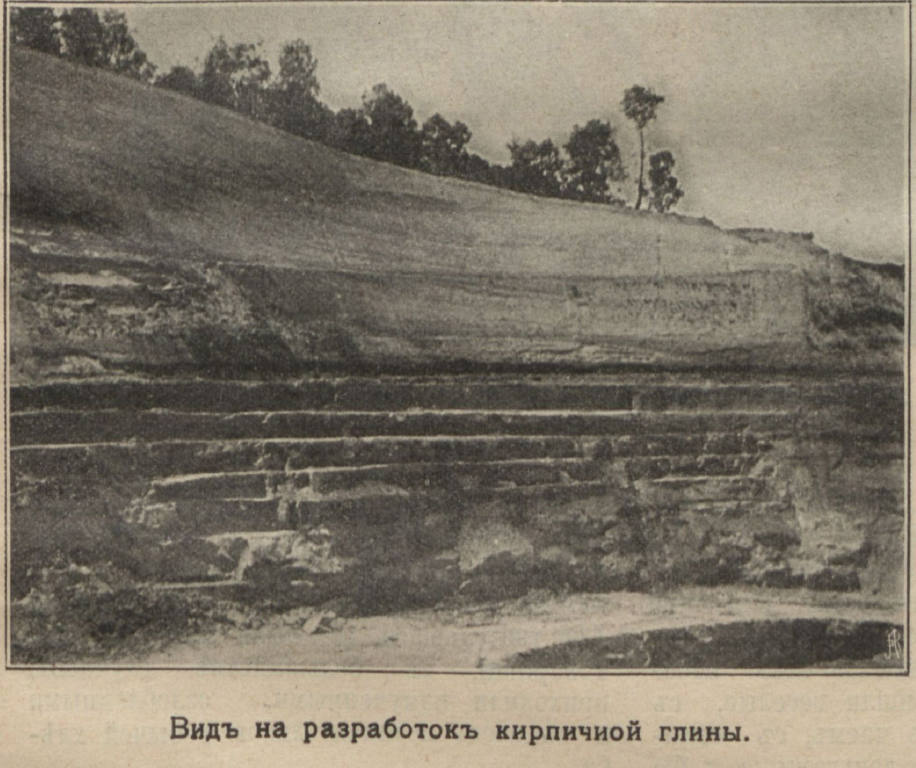
\includegraphics[width=0.91\linewidth]{pix/1910-01.jpg}
\end{center} 


\begin{center}
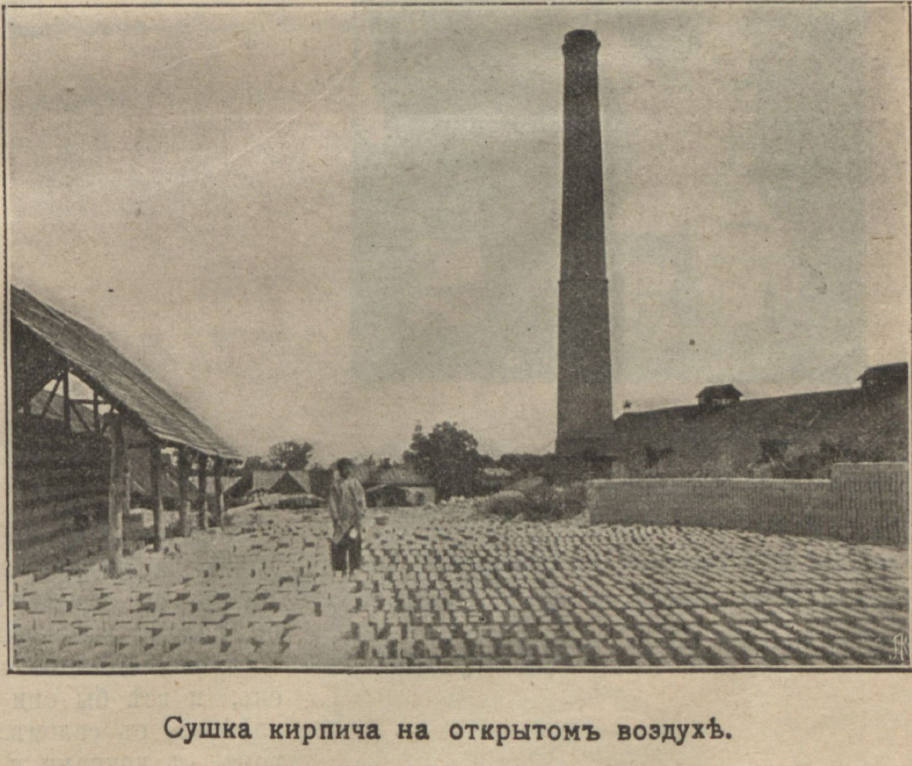
\includegraphics[width=0.91\linewidth]{pix/1910-02.jpg}

\textit{1910, фото из приложения к газете «Киевская мысль».}
\end{center} 

\newpage

\begin{center}
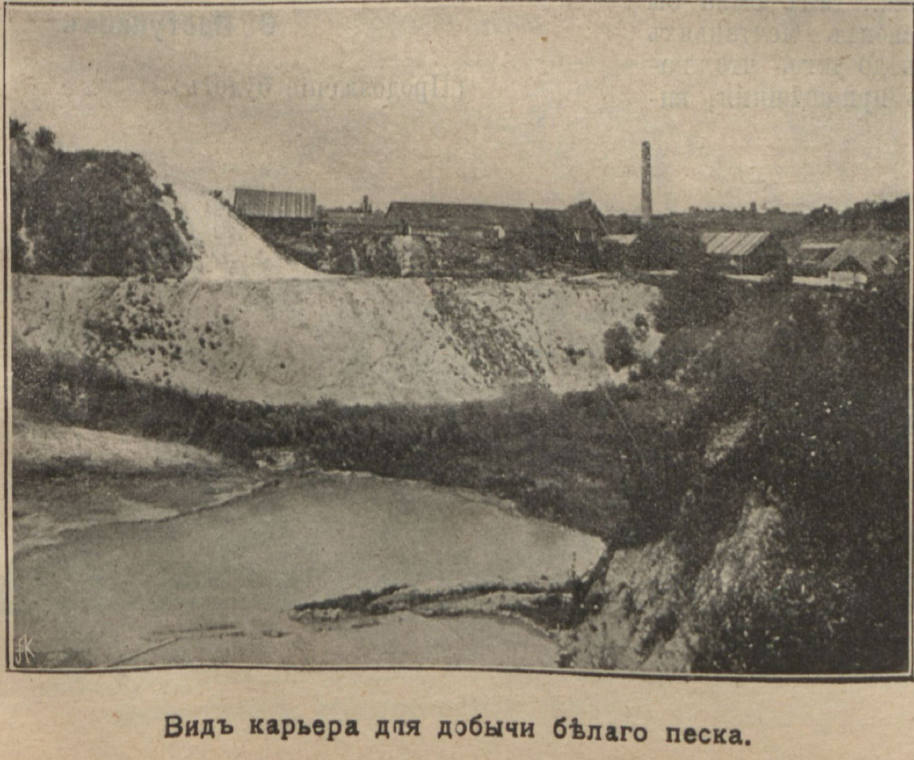
\includegraphics[width=0.91\linewidth]{pix/1910-03.jpg}
\end{center} 


\begin{center}
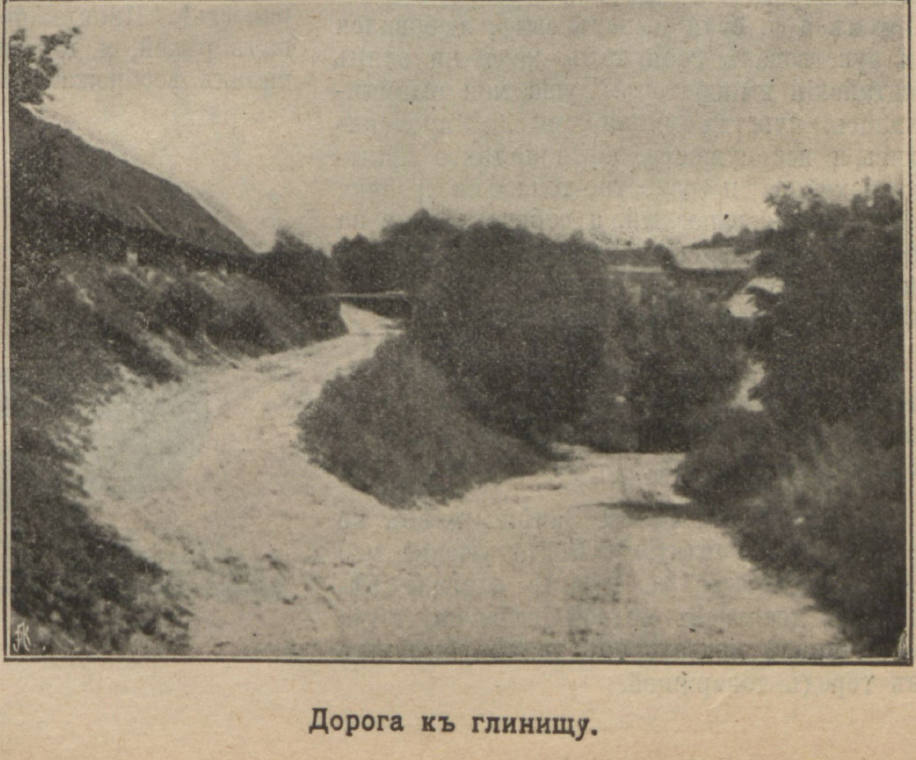
\includegraphics[width=0.91\linewidth]{pix/1910-04.jpg}

\textit{1910, фото из приложения к газете «Киевская мысль».}
\end{center} 

%\newpage
%\vspace*{\fill}
%\begin{center}
%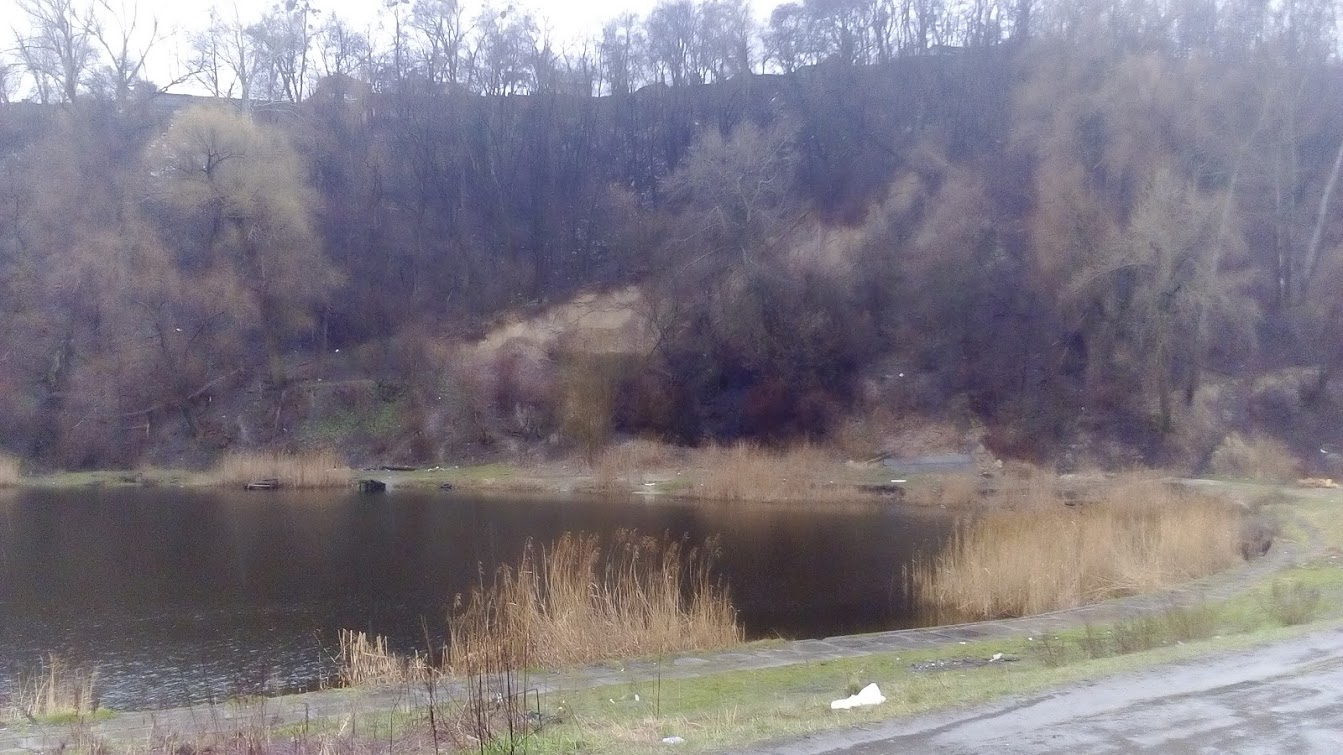
\includegraphics[width=\linewidth]{pix/DSC_0225.JPG}
%\end{center} 

%\begin{center}
%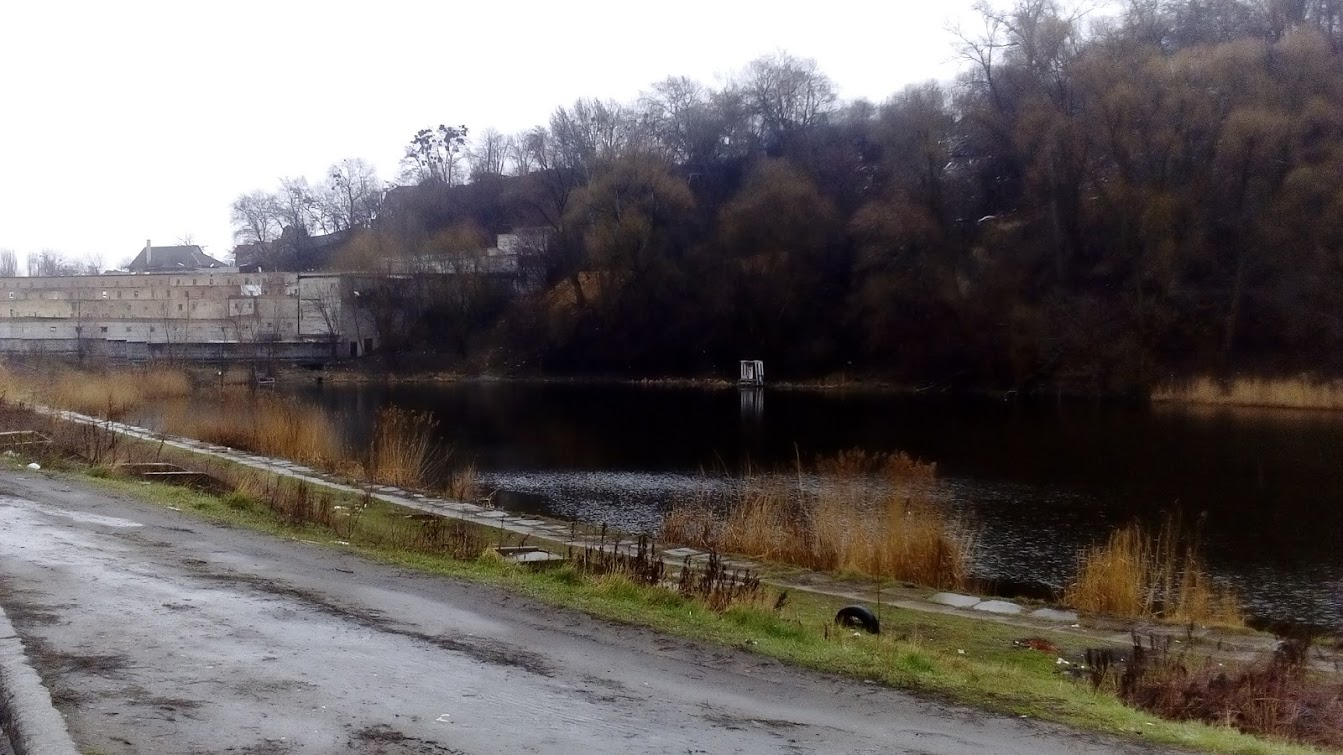
\includegraphics[width=\linewidth]{pix/DSC_0224.JPG}
%\end{center} 

%\textit{2016. Озеро в глинище на юго-запад от перекрестка Сырецкой и Копыловской. Это карьер второй половины 20 века, дореволюционные заводы кушали холм ближе к перекрестку. Фото Кати Клюевой.}
%\vspace*{\fill}
\newpage
\vspace*{\fill}
\begin{center}
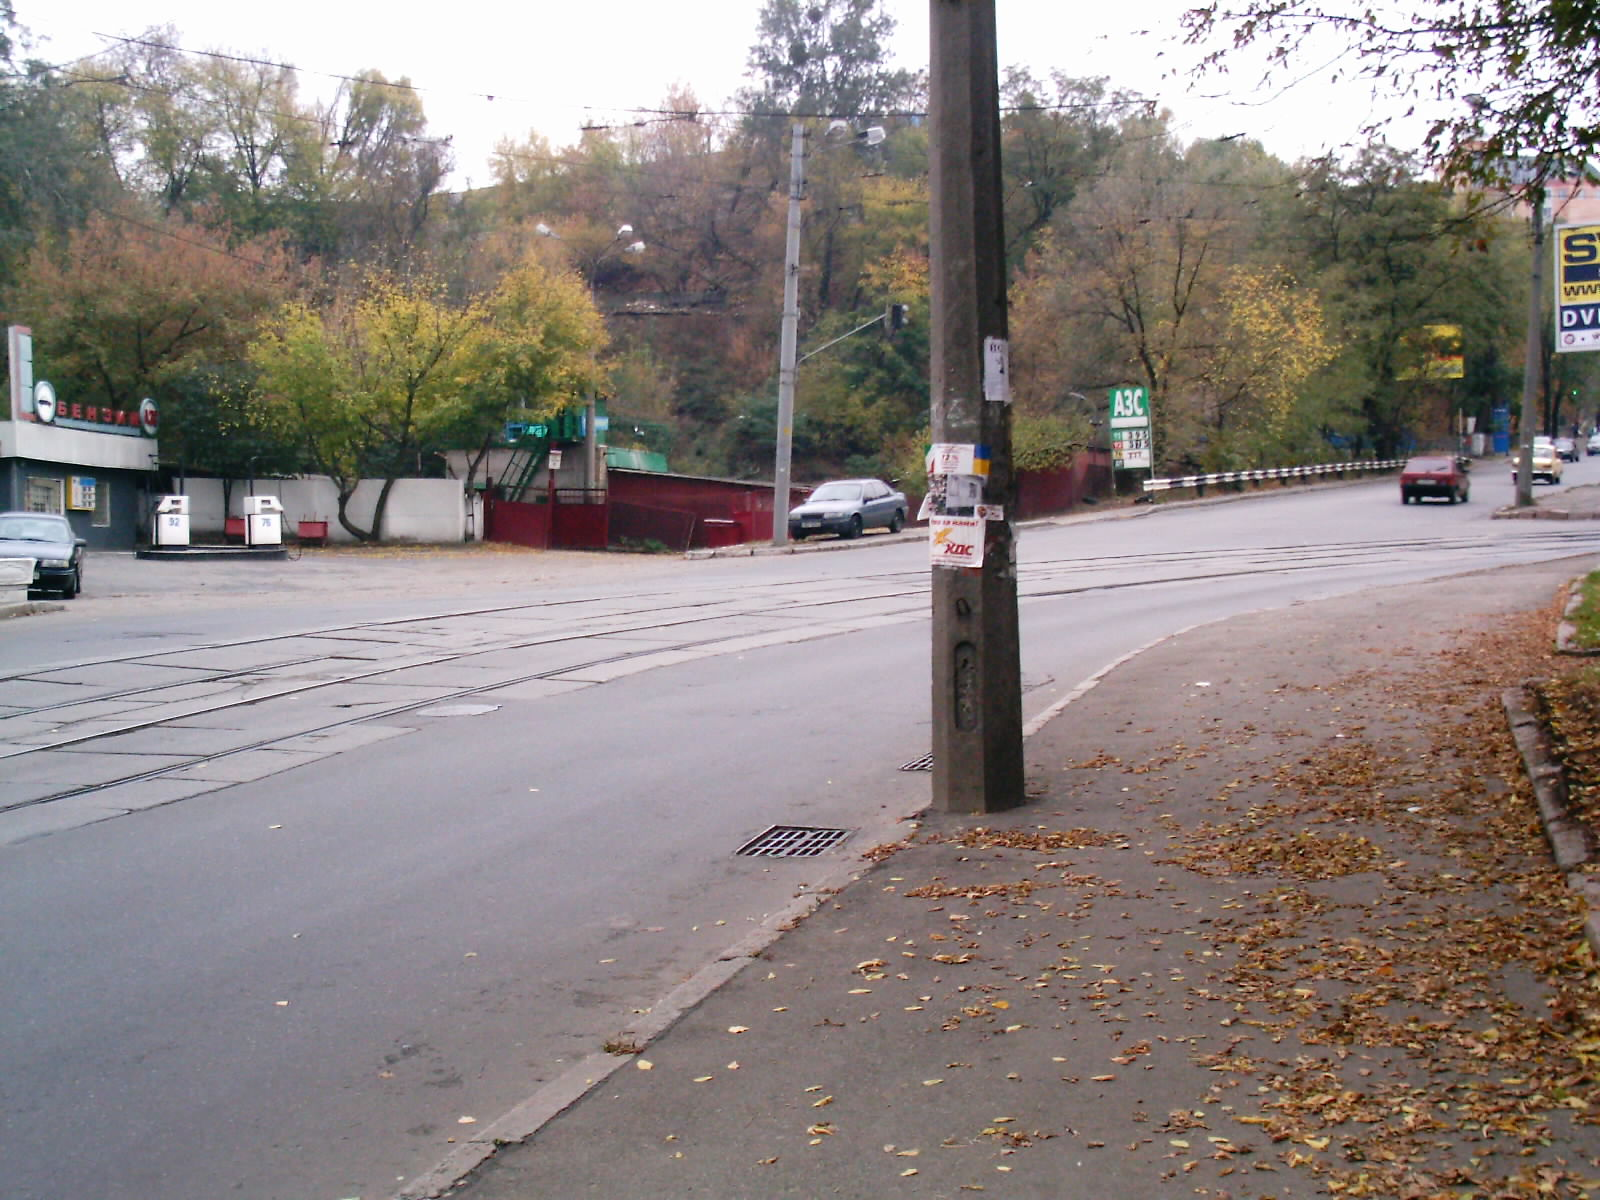
\includegraphics[width=0.90\linewidth]{pix/imag0002.jpg}

\textit{2005. Вероятно, место глинища Ясногурского.}
\end{center} 

\begin{center}
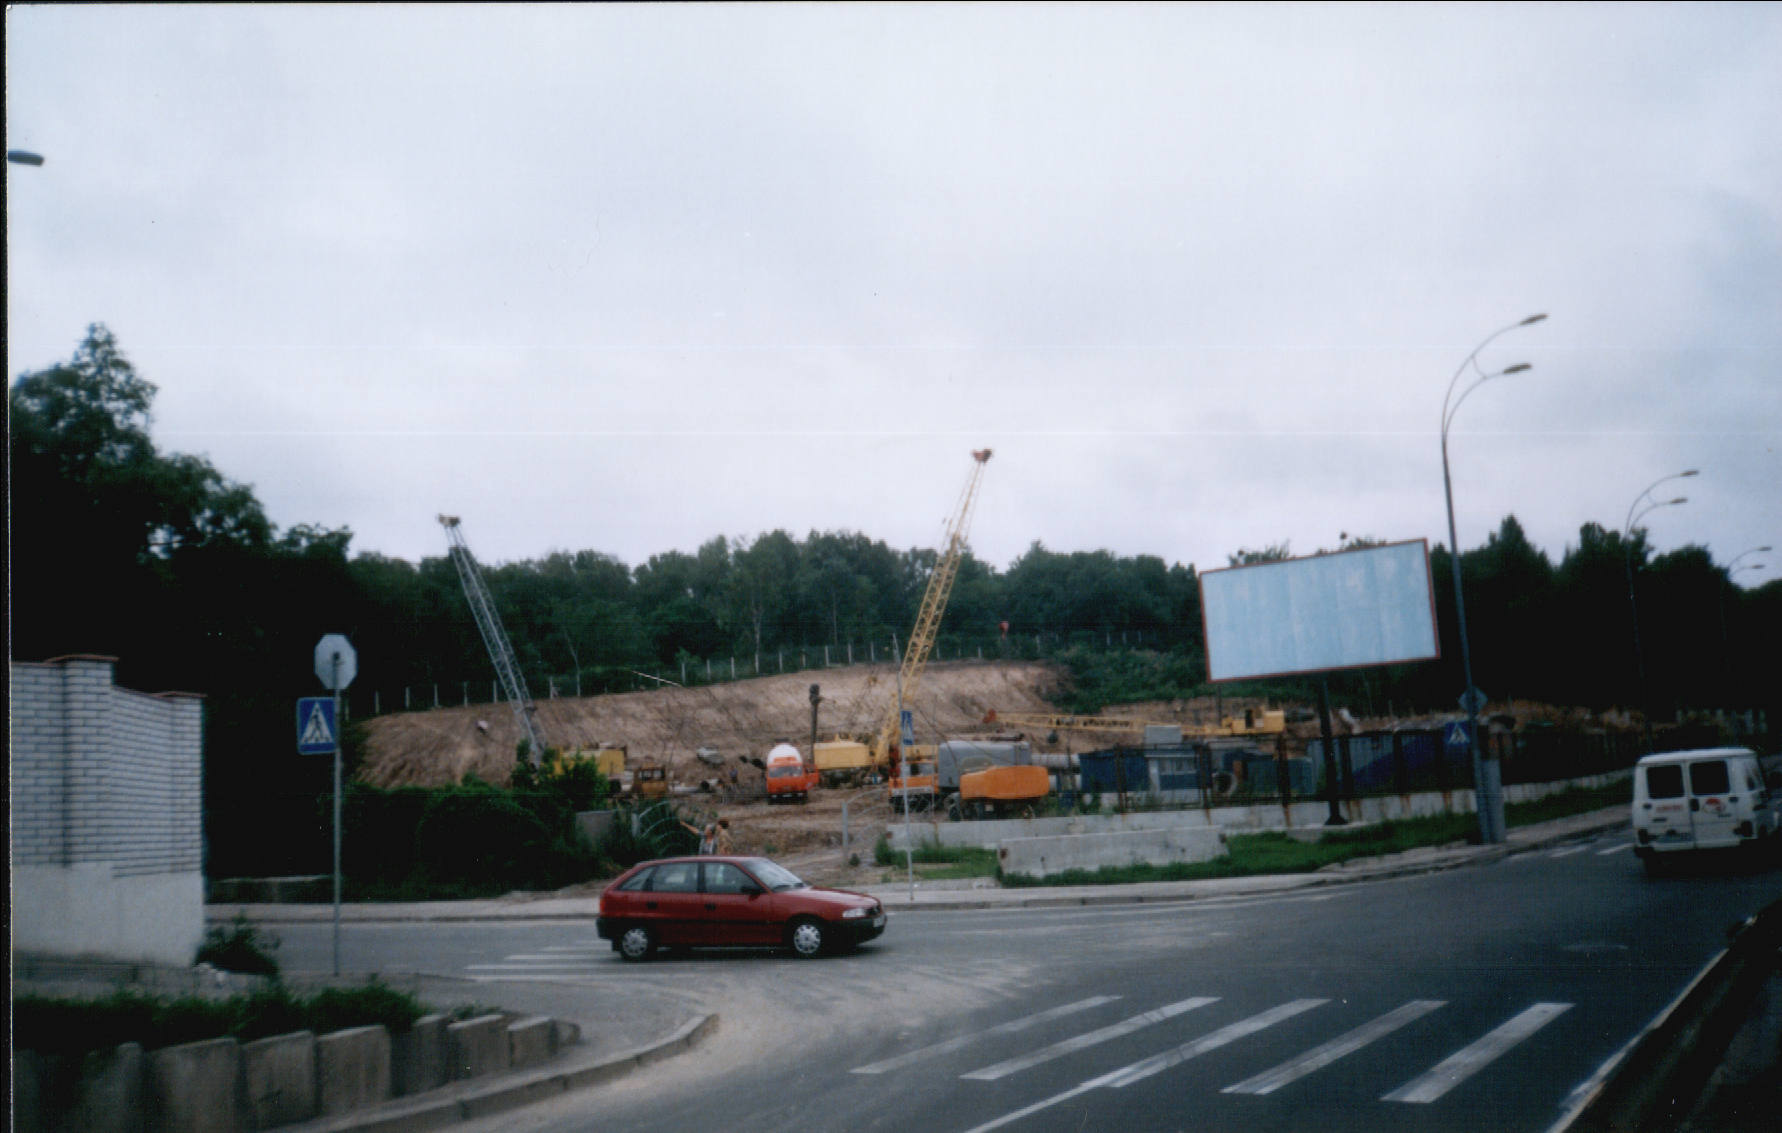
\includegraphics[width=0.90\linewidth]{pix/out0011.jpg}

\textit{2003. Застройка глинища одного из казенных заводов, южный конец Зверинецкого холма.}
\end{center} 
\vspace*{\fill}
\newpage
\vspace*{\fill}
\begin{center}
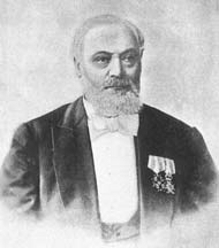
\includegraphics[width=0.60\linewidth]{faces/berner.jpg}

\textit{Бернер Яков.}
\end{center} 

\begin{center}
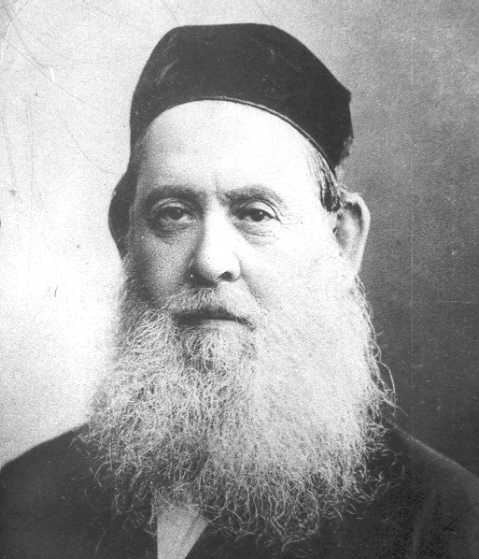
\includegraphics[width=0.60\linewidth]{faces/zajcev.jpg}

\textit{Зайцев Иона.}
\end{center} 

\vspace*{\fill}
\newpage

\begin{center}
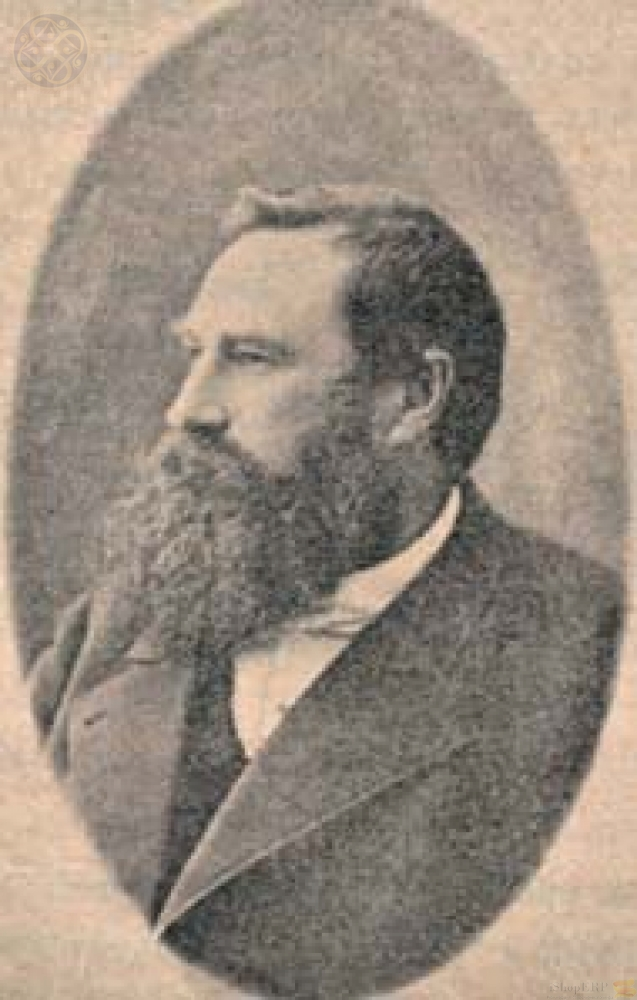
\includegraphics[width=0.50\linewidth]{faces/mihelson.jpg}

\textit{Михельсон Фридрих.}
\end{center} 

\begin{center}
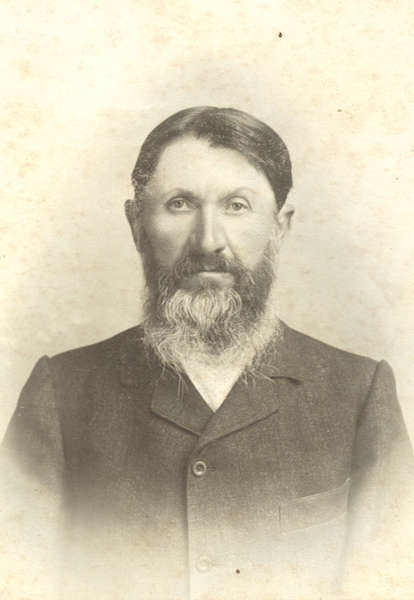
\includegraphics[width=0.50\linewidth]{faces/slepushov.jpg}

\textit{Слепушов Андрей.}
\end{center} 

\newpage
\begin{center}
\includegraphics[width=0.96\linewidth]{pix/\myimgprefix IMG_20161116_114943.jpg}


\textit{Плинфа, найденная у подножия северо-восточного мыса Зверинецкого холма, на склоне за забором ботсада примерно за остановкой «улица Выдубицкая». Окрестности известны археологам по находкам остатков гончарной слободы времен Великого Княжества Литовского и остатков здания «великокняжеского времени», которое наука отождествляет с Красным двором князя Всеволода.}
\end{center} 

\newpage

\begin{center}
\includegraphics[width=\linewidth]{pix/\myimgprefix IMG_20161116_114920.jpg}

\textit{Та же плинфа с обратной стороны.}
\end{center} 

\begin{center}
\includegraphics[width=\linewidth]{pix/\myimgprefix IMG_20161116_114743.jpg}

\textit{Другая плинфа.}
\end{center} 


\newpage


\begin{center}
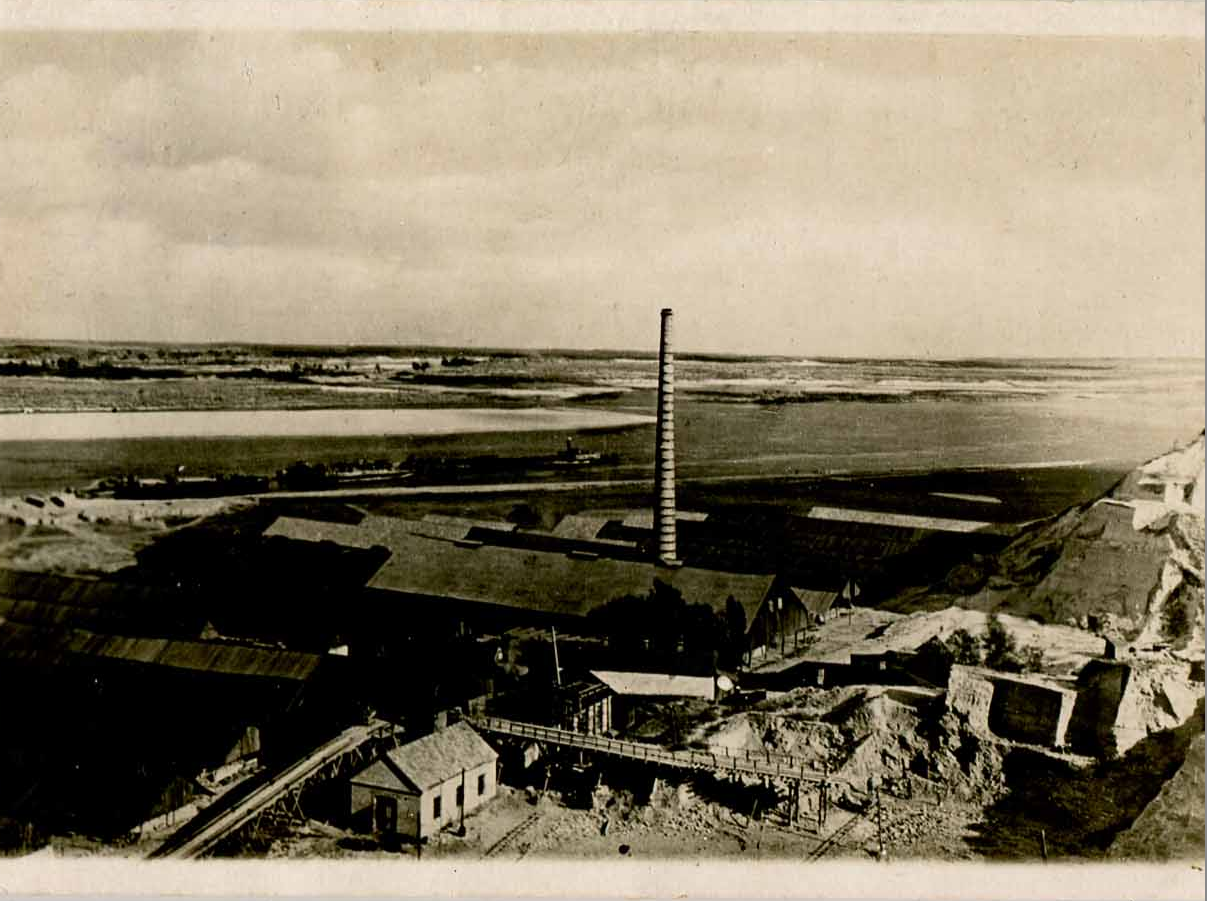
\includegraphics[width=0.95\linewidth]{pix/staiki.png}

\textit{Кирпичный завод в с. Стайки. Советская открытка.}
\end{center} 


\begin{center}
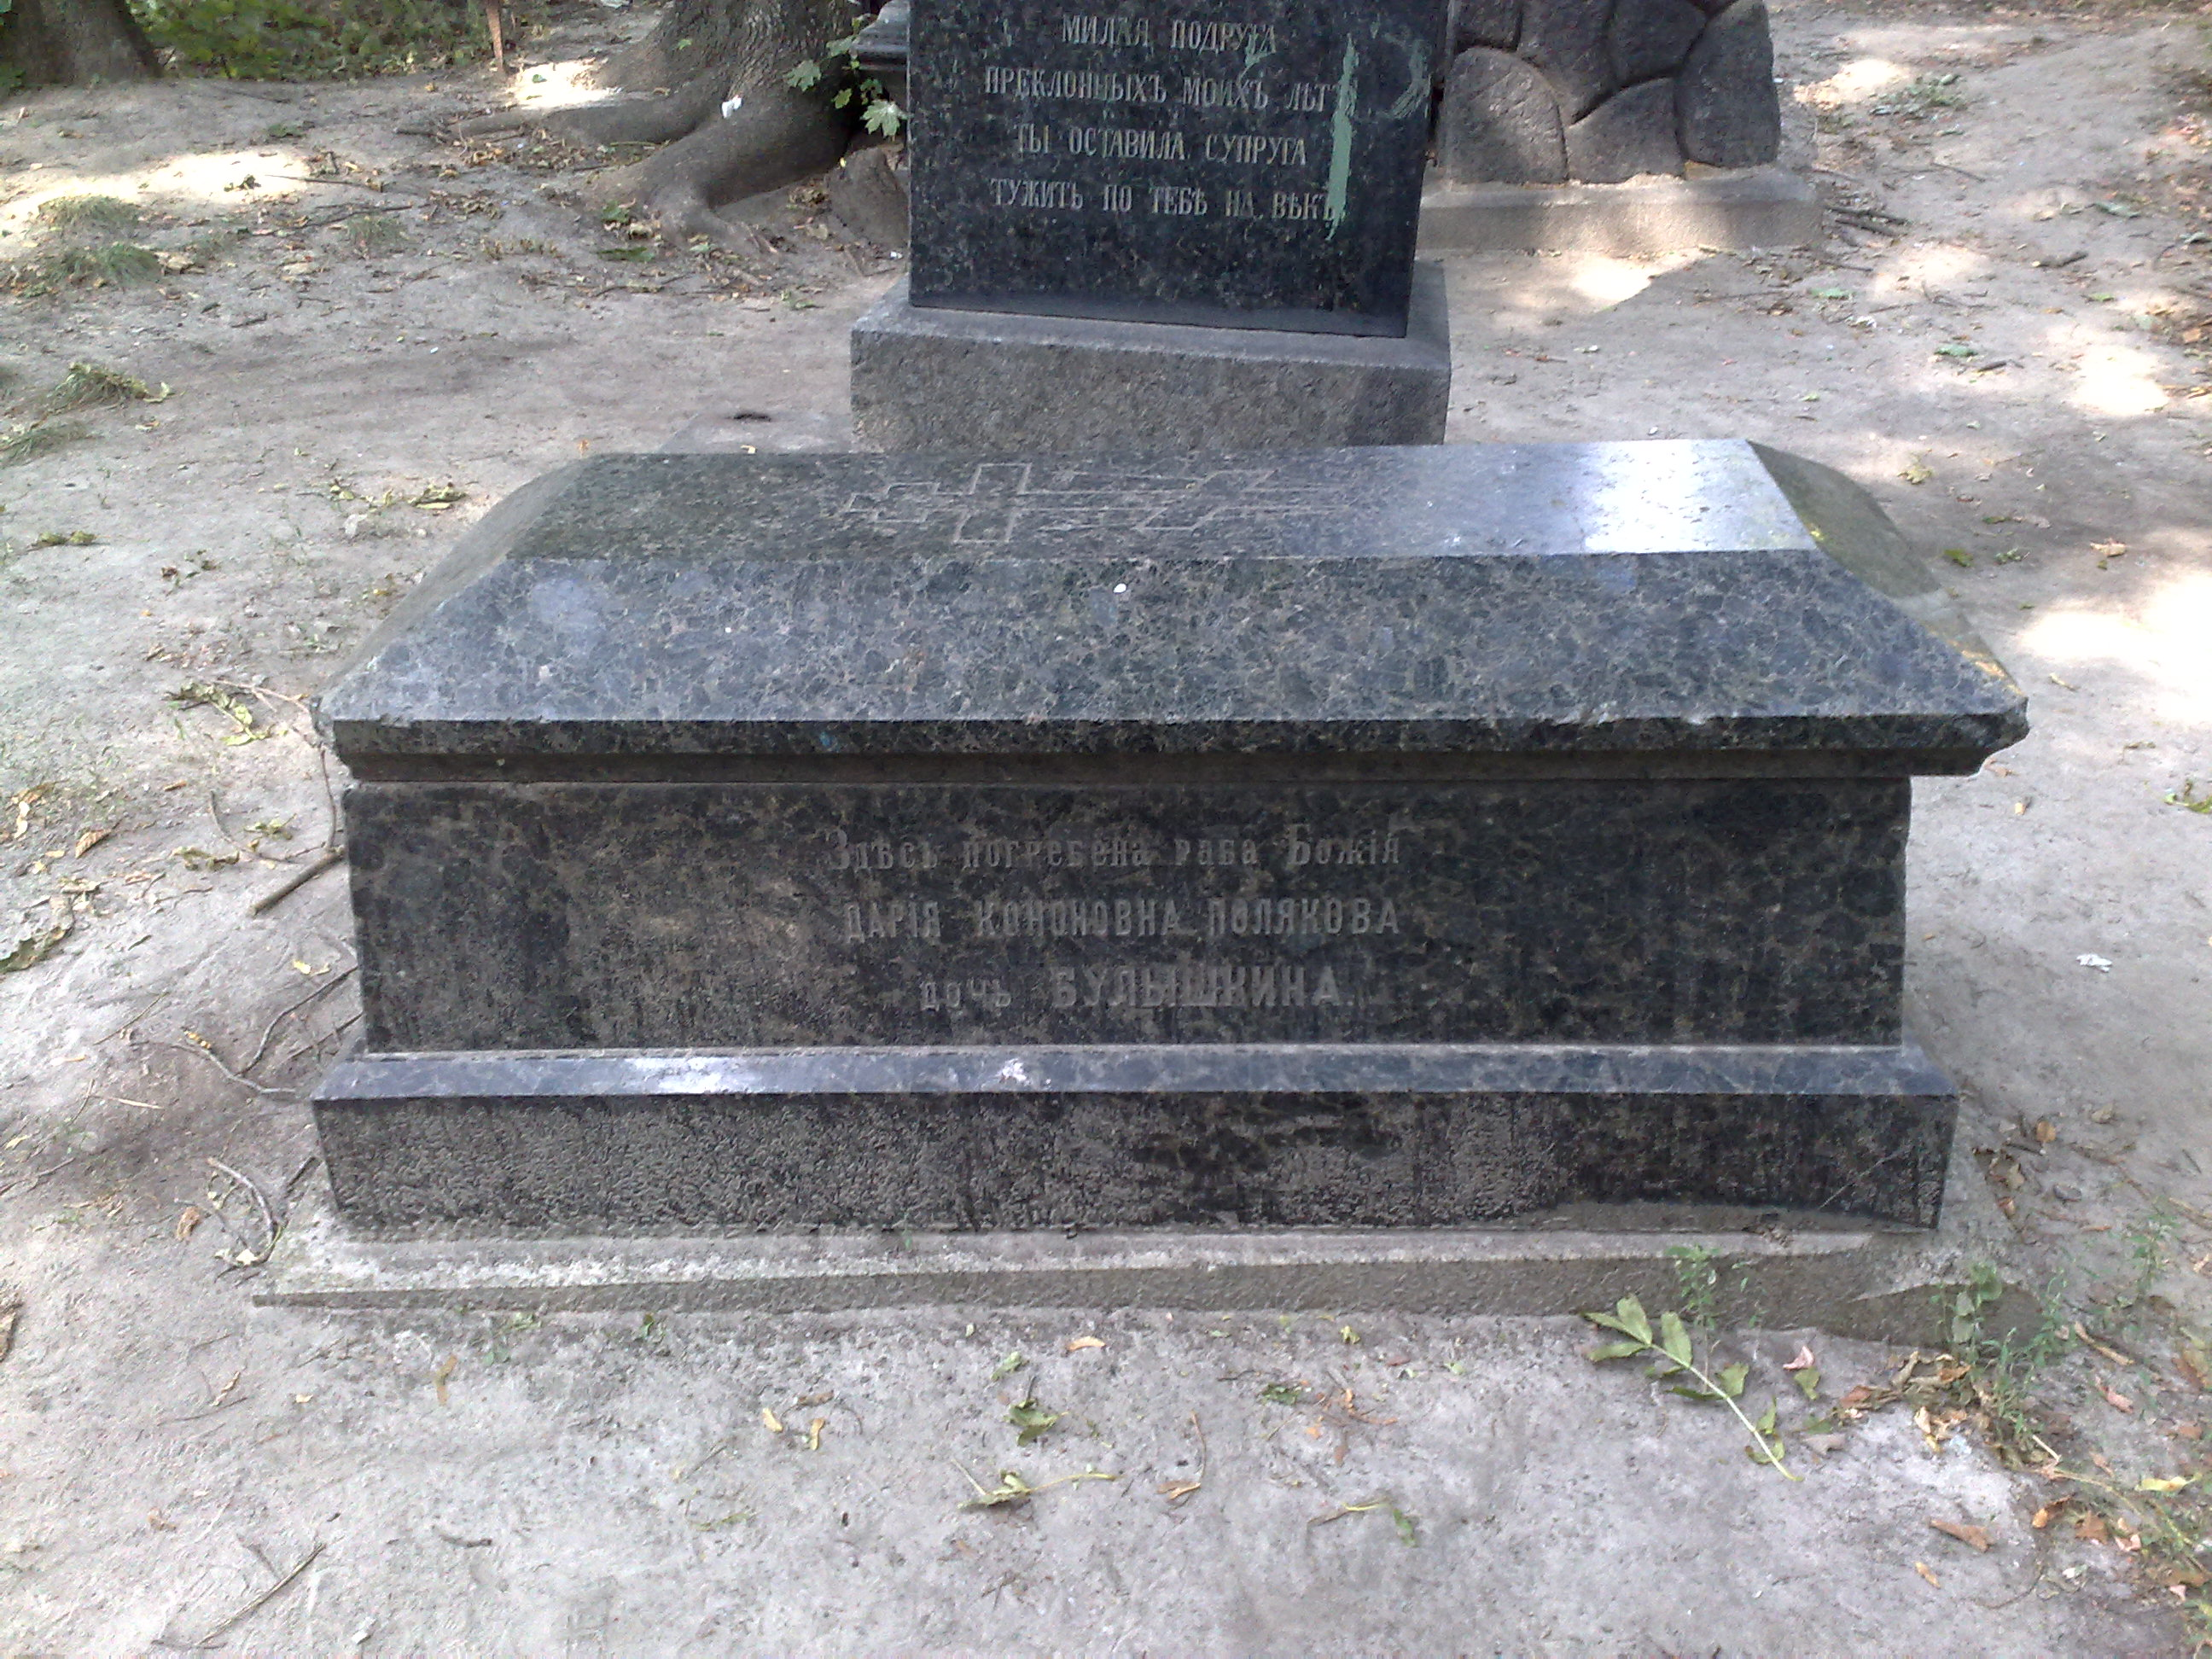
\includegraphics[width=0.95\linewidth]{pix/27082009561.jpg}

\textit{Могилы семьи Булышкиных находятся в Киеве, на старообрядческом кладбище при горе Щекавице.}
\end{center} 


\backmatter

\part*{Приложения}
\addcontentsline{toc}{part}{Приложения}

\chapter*{О кирпичной глине}
\addcontentsline{toc}{chapter}{О кирпичной глине}

\textbf{Из «Статистическое описание Киевской губернии», часть 1, издание Фундуклея (1852)}:\\

Кирпичная глина. Она находится в изобилии во всех уездах губернии, особенно в степных, но лучшая из них в г. Киеве и его окрестностях, а также возле Межигорской фабрики в с. Петровцах. В Киеве главные места разработки этой глины находятся в крутом обрыве гор, идущих вдоль низменной улицы, называемой Плоскою. Там выказывается наружу толстый пласт ее, первый снизу; на котором лежат все прочие пласты тех гор. 

Сырые кирпичи из этой глины зеленоватого светлого цвета, но будучи обожжены, принимают светло-красноватый вид. Качеством они очень хороши, особенно для кладки печей, но процент утраты при обжигании довольно значителен. В окрестностях города, особенно за Печерскою частью, кирпич выходит еще доброкачественнее, желтоватого цвета, и употребляется в значительном количестве на крепостные постройки. На некоторых низменных, ровных местах, прилегающих к Днепру, по Оболони, попадается красно-бурая глина, из которой кирпич выходит темнокрасный, и тоже очень доброкачественный. Но Межигорская глина еще лучше Киевских. Из нее приготовляется кирпич беложелтоватого цвета, особенно годный для стен фундаментов, ибо упорен против влияния влажности, обстоятельство немаловажное для Подольской и плоской части г. Киева, часто, затопляемых весной разливом Днепра.

Там же приготовляют еще другой сорт кирпича, малого формата, совершенно белый, уподобляющийся сахарным плиткам и употребляемый на выкладку пода в печах и на самые печи; глина, из которой его делают – весьма огнеупорна. Там же добывают кафельную или изразцовую глину, которую привозят и на Киевские заводы в сыром виде, для обработки.[...]

Горшечная глина находится во многих уездах, и преимущественно в Киевском и в Таращанском, при устье р. Лыбеди в Киеве и в Межигорье; [...] Кроме посуды из нее приготовляют доброкачественные изразцы для печей.[...]

Фаянсовая глина находится целыми слоями в окрестностях г. Киева при устье р. Лыбеди, но еще в значительнейших массах и лучшего качества возле Межигорской фаянсовой фабрики.\\


\textbf{«Химическое исследование киевских глин», С. Богданов, Записки Киевского общества естествоиспытателей, том 7, выпуск 1 (1883):}\\

Киевская синяя (спондилувая, кирпичная) глина\footnote{«Образец для исследования был взят на кирпичном заводе г. Субботина» – прим. С. Богданова).}.

Киевская синяя глина принадлежит второму ярусу киевской третичной эосеновой формации. На площади Киева она залегает на уровне Днепра, образуя подошву поверх лежащих более новых третичных образований.

Во влажном состоянии она имеет темно-зеленый цвет, при высыхании же зеленовато-серый; кирпич из нея приготовленный – светло-желтого цвета. Влажная глина мягка, с слабым блеском; липнет к языку. Ломается синяя глина глыбами, имеющими широко-раковистый землистый излом и плоскость разреза с матовым блеском. В воде отчасти листится и распускается трудно, не производя мути; при этом наблюдается обильное выделение пузырьков воздуха, сопровождающееся характерным шумом (в роде свиста).

Смоченная глина имеет довольно ясный аммиачный запах. При действии кислот сильно шипит вследствие обильного выделения пузырьков углекислоты. Макро и микроскопическое исследование, кроме глинистой части, окрашенной примесью бурого железняка, обнаруживает еще кварцевый песок, блестки сере\-бристо-белой слюды и мелкие зерна главконита. В некоторых образцах синей глины можно также заметить мелкие желваки железного колчедана, мергельные сростки, содержащие фосфорно-известковую соль, и наконец обыкновенно кристаллы гипса. Значительного количества полевого шпата не видно (сообщено К. М. Феофилактовым). При отмучивании уже самые первые порции, состоящие из наиболее мелких частиц, окрашены в зеленоватый цвет и содержат некоторое количество кварцевого песка.

Объем 1 gr. сухой глины, вобравшей в себя возможное количество воды, равен 1,9 c.c.m. (среднее из двух чисел: 1,84 c.c.m. и 1,91 c.c.m.). Водоемкость 1,3 (среднее из двух чисел: 1,24 и 1,30). Maximum гигроскопичности 6,69 (среднее из двух чисел: 6,78 и 6,61). Таким образом синюю глину следует признать весьма пластичною.

При накаливании приготовленного из нея цилиндрика уже при 1000° C. происходит настоящее плавление, следовательно она весьма легкоплавка. С этим выводом вполне гармонирует и ничтожный коэффициент огнеупорности синей глины, равный 0,02.

Употребляется синяя глина на многочисленных киевских кирпичных заводах для изготовления строевого кирпича прекрасных качеств.

Первый полный элементарный анализ ея принадлежит г. Рожанскому\footnote{«Зап. К. О. И. Р. Т. О. 1881, XI, 11» – прим. Богданова.}, важнейшие результаты которого потом подтвердил г. Марциновский\footnote{«Частное сообщение. Аналиы гг. Рожанского и Марциновского были произведены также в Технической лаборатории Университета св. Владимира» – прим. Богданова.}, и вследствие этого отсутствие необходимости повторять их исследование. Таким образом я занялся преимущественно вопросом о ближайших составных частях этой глины. Результаты всех указанных выше элементарных анализов синей глины представляет следующая таблица.


\begin{center}
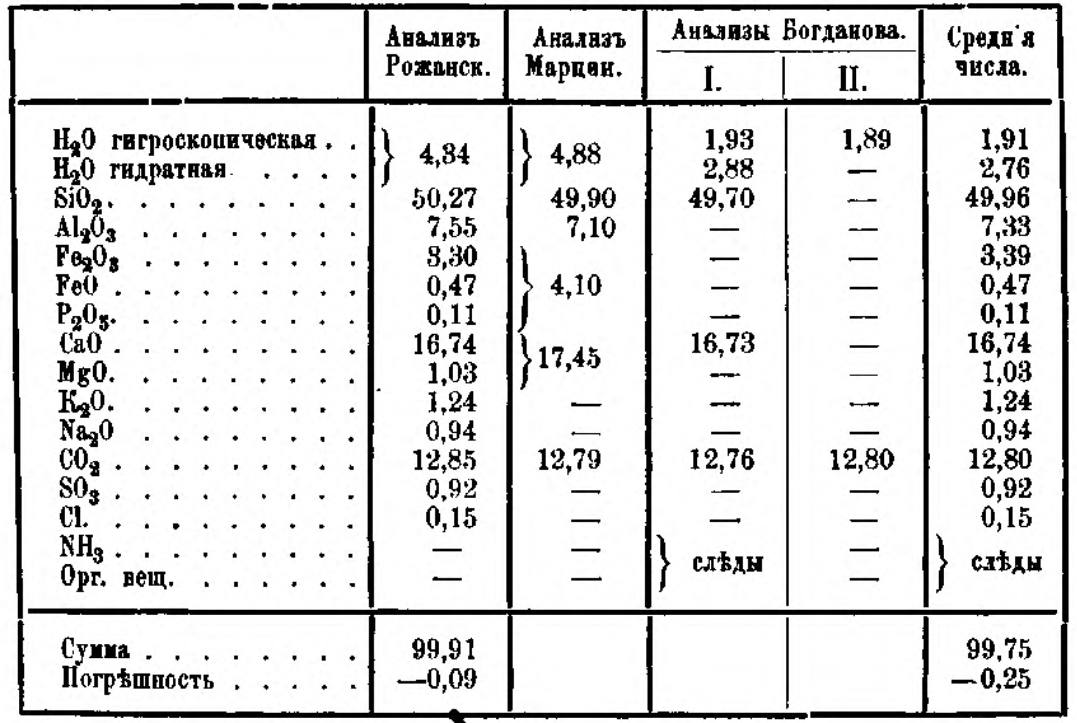
\includegraphics[width=\linewidth]{pix/table-01.jpg}
\end{center} 

В анализах гг. Рожанского и Марциновского не приведены отдельные числа для H$_2$O гигроскопической и гидратной, потому что эти исследователи принимаю за гигроскопическую воду в глинах потерю, претерпеваемую последними выше 120° C., что несогласно с изложенным выше моим взглядом на этот предмет.

Содержание в синей глины разных видов химически соединенной воды по моим определениям, следующее:\\


\begin{tabular}{| l | l |}
\hline
H$_2$O непрочно соед. & 0,96 \\
H$_2$O прочн. соедин. & 1,80 \\
\hline
\end{tabular}\\

(К 1,80 Богданович делает примечание: «Найденная гг. Рожанским (2,86\%) и Марциновским (2,92\%) потеря синей глины при 120° C., равная сумме гигроскопической и непрочно соединенной воды весьма близко подходит к той же сумме, составленной на основании моих определений (0,96\%+1,80\%=2,76\%)»).

Из общего количества SiO$_2$, по определению г. Рожанского, в синей глине заключается\\

\begin{tabular}{| l | l |}
\hline
Кварцевого песка & 32,03\\
SiO$_2$ химич. соедин. & 18,24 \\
\hline
\end{tabular}\\

(К 32,03 Богданович примечает: «Определяется нагреванием глины с серной кислотой в запаянной трубке и т.д., как в пестрой глине».)

При произведенных же мною и г. Марциновским опытах кипячения глины с серной кислотой в платиновой чашке, с последующей обработкой нерастворимого остатка кипящим раствором соды, получилось:\\

\begin{center}
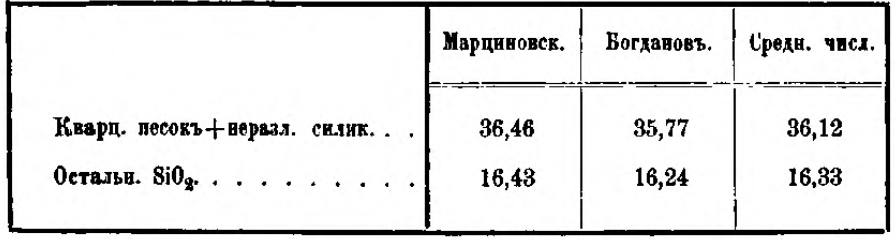
\includegraphics[width=\linewidth]{pix/table-02.jpg}
\end{center} 

Вычитая из суммы кварцевого песка + неразложившийся силикат полученное г. Рожанским число для чистого кварцеватого песка, я нахожу, что силикат, неразлагаемый кипящею серною кислотою при атмосферном давлении, заключается в синей глине в количестве 4,09\%. Если же от суммы кварцеватого песка + неразложившийся силикат + остальной SiO$_2$ (равной 52,45\%) отнять общее содержание SiO$_2$, то окажется, что основания в указанном силикате составляю 2,49\%.

Относительно природы этого соединения можно сделать заключение уже на основании микроскопического исследования синей глины, так как из всех найденных в ней этим способом силикатов лишь поташистая слюда не разлагается серною кислотою при кипячении в открытом сосуде. И микроскопическое исследование нерастворимого остатка, полученного при моем опыте, указывает на присутствие здесь кварца и слюды (сообщение г. Армашевского). Приняв для поташистой слюды типическую формулу K$_2$O. Al$_2$O$_3$. 2SiO$_2$, я, по общему содержанию оснований, нахожу, что K$_2$O в поташистой слюде синей глины составляет 1,18\%, Al$_2$O$_3$ 1,31\%, SiO$_2$ 1,51/%.

Отнимая сумму оснований + вычисленное количество SiO$_2$, слюды от суммы кварцевого песка + неразложившийся силикат, я определяю непрямым способом содержание чистого кварцевого песка в синей глине, которое оказывается равным 32,12\%, – число весьма близкое к найденному г. Рожанским, что указывает на правильность оснований его определения и, вместе с тем, на правильном допущения в нерастворимом в серной кислоте остатке глины только кварца и поташистой слюды.

Взяв средние числа из всех прямых и непрямых определений кварцевого песка в синей глине и приняв остальной SiO$_2$ <ся>  за химически соединенный, нахожу, что здесь содержится\\ 

\begin{tabular}{| l | l |}
\hline
Кварцевого песка & 32,08 \\
SiO$_2$ химич. соедин. & 18,88 \\
\hline
\end{tabular}\\

Среднее же содержание поташистой слюды нужно выразить числом 4,0\%, которое впрочем следует считать только приблизительным, так как определение поташистой слюды основано на допущении совершенной неразлагаемости ея при кипячении с серной кислотой в платиновой чаше, так как она при этом уже несколько разлагается.

При определении прочих ближайших составных частей синей глины гораздо более важное значение, чем для двух предыдущих глин, имеет обработка ея разными реактивами. Так, уже вода извлекает из синей глины довольно значительное количество примесей: следы органических веществ, немного Cl, Na и довольно много CaO и CO$_3$.

На основании этих данных я заключаю о присутствии в синей глине небольших количеств NaCl и органических (вероятно, как и в предыдущих глинах, частью в виде известковых солей перегнойных кислот), а также значительного количества гипса, общее содержание которого определяю на том основании, что после обработки водою в глине уже не оказывается SO$_3$, который следовательно, весь входит в состав гипса. Таким образом в последнем заключается SO$_3$ – 0,92\%, CaO – 0,64\%, 2H$_2$O – 0,41\%, общее же количество гипса равно 1,97\%. Обе частицы воды гипса принадлежат к непрочно соединенной воде глины, так что на прочие составные части синей глины остается воды непрочно связанной всего 0,55\%.

Общее содержание NaCl определяется количеством Cl, заключающегося только в NaCl: Cl – 0,15\%, Na – 0,09 – NaCl составляет таким образом 2,24\%.

Уксусная кислота на холоду выделяет из синей глины CO$_2$, и извлекает в раствор очень много CaO меньше MgO, немного Fe$_2$O$_3$, Al$_2$O$_3$ и SiO$_2$, также весьма мало P$_2$O$_3$. После этой обработки в глине остаются только следы P$_2$O$_3$, которые извлекаются соляной кислотой, так что, принимая во внимание преимущественное распространение в природе из фосфатов, разлагаемых уксусною кислотою – известкового, а из неразлагаемых уксусной кислотой, но поддающихся действию соляной кислоты – фосфата Fe$_2$O$_3$, следует заключить о присутствии в синей глине некоторого количества Ca$_3$(PO$_4$)$_2$ и следов FePO$_4$. Fe$_3$(PO$_4$)$_2$ в исследуемой глине нет, так как уксусно-кислая вытяжка не заключает вовсе FeO. Относя весь P$_2$O$_3$ к Ca$_2$(PO$_4$)$_2$ и пренебрегая ничтожным количеством его в виде FePO$_4$, получаю, что в синей глине Ca$_3$(ЗЩ$_4$)$_2$ составляет 0,26\% (P$_2$O$_5$ – 0,11\%, CaO – 0,15\%).

Принимая во вниманием, что после обработки уксусной кислотой в глине не остается сколько-нибудь значительного количества CaO, я считаю возможным всю остальную CaO, кроме заключающейся в гипсе и Ca$_3$(PO$_4$)$_2$, т.е. 15,59\%, отнести к CaCO$_3$; в таком случае в этой соли заключается CO$_2$ 12,53\%, общее же количество CaCO$_3$ синей глины равно 28,48\%.

Остальная CO$_2$ (2,27\%) соединена с MgO, так что количество MgO$_3$ равно 0,52\%.

Правильность выводов относительно общего содержания в синей глине CaCO$_3$, MgCO$_3$, гипса и Ca$_3$(PO$_4$)$_2$ подтверждается тем, что при обработке глины уксусной кислотой до прекращения вы <далее у меня нет страниц>[...]

Например, киевская синяя глина, содержащая около 4\% бурого железняка, при слабом прокаливании окрашивается в желтый цвет, но при более высоких температурах, когда начинается сплавление глины, она получает черную окраску, что вероятно зависит от главконита, который в чистом состоянии показывает ту же особенность.[...]

Еще меньше коалина в киевской синей глине (около 10\%), главные составные части которой – кварцевый песок (32\%) и CaCO$_3$ (28 1/2\%), так что синюю глину правильнее называть песчаным мергелем. Зеленоватый цвет ея зависит от присутствия около 2\% главконита. Она весьма пластична и легкоплавка.

\chapter*{Из Киевлянина №254, 1898}
\addcontentsline{toc}{chapter}{Из Киевлянина №254, 1898}

\textbf{Кирпичные заводы Киева и окрестностей, часть IV}

Из кирпичных заводов долины Лыбеди в самых благоприятных условиях относительно сбыта кирпича находятся заводы Я.Н. Бернера, В.А. Субботина и наследников г-жи Шатовой. Так как они расположены в конце Большой Васильковской улицы, то при доставке кирпича покупателям пользуются городскою мостовую. Поэтому, в то время как другие заводы, находящиеся вне городской черты, принуждены во время весенней и осенней распутицы приостанавливать на некоторое время доставку кирпича в город, распутица не причиняет почти никаких хлопот трем вышеупомянутым заводам.

Завод Я.Н. Бернера имеет 12 столов и 1 Гофманскую печь в 16 камер, вместимостью в 200 000 штук кирпича. Заводу принадлежит около 9 десятин земли и глинище его находится весьма близко от сараев, в которых производится выделка кирпича. Завод вырабатывает в год 4 1/2 – 5 млн. кирпича и на нем работает до 100 чел. рабочих и свыше 60 лошадей, доставляющих глину к милкам и месящих ее.

Завод В. Субботина по размерам производства почти в полтора раза превышает завод Я.Н. Бернера и его производительность превышает 6 млн. штук кирпича ежегодно. Заводу принадлежит обширная площадь земли и, несмотря на то, что принадлежащий ему пласт глины эксплоатируется уже более 60 лет, до сих пор разрыта лишь ничтожная часть территории завода. Заводу приходится производить довольно значительную съемку земли и его глинище представляет собой довольно глубокий овраг. На заводе имеются две гофманские печи. Количество рабочих превышает 130 человек и, кроме того, на заводе работает около 80 подвод. 

Завод В.А. Субботина относится к числу самых благоустроенных кирпичных заводов в окрестностях Киева. Он имеет массу древесных насаждений и весь утопает в зелени. Для рабочих устроены специальные казармы, представляющие собой капитальное каменное здание. На других заводах помещения для рабочих отличаются чрезмерной простотой и представляют собой часто ряд отдельных небольших каморок, приютившихся, наподобие ласточкиных гнезд, под навесом гофманской печи. Сами рабочие мало разборчивы на счет помещения\footnote{Ну да, как же. Что хозяин завода предоставит, там и живут.}, ютятся часто в сараях, в пещерах, спят прямо под открытым небом.

Завод наследников г-жи Шатовой помещается рядом с заводом В.А. Субботина и его усадьба представляет собой узкую возвышенную полосу земли, тянущуюся вдоль Васильковской дороги. Производительность завода не велика, благодаря тесноте места, и он выделывает всего не более 2 млн. кирпича в год. Гофманская печь рассчитана на 80 000 штук кирпича. Число рабочих не превышает 50 человек.

Три вышеописанных хавода расположены по соседству друг от друга в конце Большой Васильковской улицы. Следующий завод долины Лыбеди, Лаврский, находится в версте от них вниз по Лыбеди. Сам завод, гофманская печь и сараи для выделки и сушки кирпича помещаются по правую сторону полотна Московско-Киево-Воронежской дороги, его глинище по левую сторону полотна, в 200 саж. от завода. Выделка кирпича производится на семи столах и составляет около 2 млн. штук ежегодно. Число рабочих превышает 60 человек.

Следуя вниз по течению Лыбеди, которая после выхода из лаврского пруда имеет крайне жалкий вид, мы попадаем на большой завод, устроенный на земле Киево-Выдубецкого монастыря и принадлежащий Я.Н. Бернеру. Прежним арендатором, Эрлихом, производилась здесь машинная выделка кирпича, в воспоминание о чем сохранилась высокая двухэтажная постройка, в которой теперь помещаются лошади и коровы. Так как завод расположен у самого подножья Лысой горы с ее фортами, то ему не разрешается возводить постоянных построек, в виду чего все сараи для просушки кирпича выстроены из самого дешеваго материала и носят временный характер.

На заводе имеются две гофманские печи, вместимостью по 200 000 кирпича каждая. Глинище расположено вблизи от центра завод аи при том оно довольно мелко, благодаря чему доставка глины в малки не представляет никаких затруднений. Благодаря этому на заводе сравнительно меньше лошадей, чем на других, и число их не превышает 50. На заводе работает до 150 человек рабочих. Он производит 7 млн. кирпича.

Завод Я.Н. Бернера отделен лишь межою от бывших казенных заводов, принадлежащих в настоящее время наследникам Снежко, которым принадлежат, вообще, около 100 десятин земли, занятой под заводские постройки вплоть до самого Китаево, или Мышеловки, к которой приписаны в административном отношении заводы. Три завода Снежко вырабатывают в общей сложности около 14 млн. кирпича. На заводах устроены четыре гофманские печи, вместимостью в 200 000 штук кирпича каждая. Выделка кирпича производится на 40 столах и число рабочих превышает 340 человек. Два завода арендуются у наследников Снежко, Фокиным и Доломашкиным, третий, самый большой, с двумя гофманскими печами, эксплоатируется непосредственно самими владельцами, при чем все годовое производство продано вперед Л. Козинскому. Завод принадлежит к числу более благоустроенных, все сараи построены из хорошего материала и содержатся в порядке.

Вторая группа кирпичных заводов, расположенных в окрестностях Киева, помещаются в долине безымянного ручья, вытекающего из пруда Голосеевской пустыни. Голосеевский пруд занимает центральную часть котловины, окруженной горами, покрытыми лесом, по преимуществу дубом, и питается ключами, берущими начало и подножья гор. Голосеевская роща, принадлежащая Киево-Печерской лавре, и Голосеевский пруд недоступны публике и малоизвестны в Киеве, в то время как по красоте положения редкая местность в окрестностях Киева может соперничать с Голосеевым.

Из этого живописнейшего озера вытекает небольшой ручеек, вливающийся в Днепр почти в том же пункте, что и Лыбедь. В прежние годы ручеек был, вероятно более многоводным и на нем стояло несколько мельниц, ни одна из которых не работает теперь за отсутствие воды в ручье, которые еще мельче Лыбеди. Долина ручья гораздо уже, чем долина Лыбеди, и берега ея гораздо круче. Вся долина на протяжении от Голосеевского леса до Китаево, или собственно Мышеловки, занята кирпичными заводами. Сараи для выделки и сушки кирпича, гофманские печи и прочие строения покрывают сплошь всю долину, глинища же их врезываются в горы берегов долины. Занимая собой узкое ущелье, заводы сильно стеснены и им расширяться уже некуда, так что приходится утилизировать каждую квадратную сажень долины ручья.

Последний представляет уже в настоящее время узкую канаву, так как болотистые, низкие берега его подсыпаются заводами и на полученном таким образом насыпном грунте возводятся все новые и новые постройки. Еще несколько лет тому назад ручей в одном пункте был запружен и образовывал второй пруд, теперь этот пруд уже почти совершенно засыпан.

Земли, расположенные по берегам ручья, принадлежат крестьянам с. Мышеловки, или ведомству государственных имуществ, у которых арендуются владельцами кирпичных заводов. В долине Голосеевского ручья расположены следующие заводы: Д.Л. Горчакова, И.С. Ясько, А.К. Рейхе, Калашникова и Лунева. В отношении эксплоатации эта группа заводов представляет то неудобство, что соединены с городом крайне неудобною, гористою дорогою, которая осенью и весной превращается в сплошное болото.

Завод Д.Л. Герчикова расположен в верхней части долины ручья на границе с дачею лавры. Выделка кирпича производится на 12 столах, число рабочих 110-120 человек, гофманская печь одна на 200 000 кирпича. Завод производит до 4 1/2 млн. кирпича.

Завод И.С. Ясько несколько меньше предыдущего и выделка кирпича производится на нем на 10 столах. Гофманская печь одна, число рабочих простирается до 100 человек. Завод производит около 3 млн. кирпича.

Завод А.К. Рейхе располагает столь незначительной площадью, что не только вся его усадьба застроена сараями, но даже пришлось утилизировать чердачное помещение над гофманской печью. Это помещение несколько повышено и в нем установлены два стола для выделки кирпича. Так как гофманская печь построена у подножия горы, то подавать кирпич в чердачное помещение не представляет особых затруднений. На заводе имеется 12 столов и его годичное производство превышает 4 1/2 млн. Число рабочих 120.

Завод Калашникова принадлежит к числу самых маленьких заводов в окрестностях Киева. Выделка кирпича производится здесь на четырех столах. На заводе 30 человек рабочих, 10 лошадей, одна гофманская печь, вместимостью 150 000 кирпича, которого завод обжигает, вообще, около 1 1/2 млн. штук.
   
На последнем заводе этой группы, Лунева, выделка кирпича производится на 11 столах. На заводе работают 85 человек и завод производит около 3 1/2 млн. кирпича.

В.Ц.
\chapter*{Цены на кирпич}
\addcontentsline{toc}{chapter}{Цены на кирпич}

Некоторые примечания.

Летний строительный сезон делился на две части – до дня Петра и Павла (29 июня по старому стилю) и после. Во второй части кирпичное производство сокращалось, а некоторые заводы вообще приостанавливали производство.

В самом конце 19 века, когда в Киеве была «строительная горячка» (при помощи банковских ипотечных кредитов), кирпич продавался по 27-28 рублей за тысячу. Возникали новые заводы, а старые увеличивали объемы производства. 

Затем строительный бум прекратился, спрос на кирпичи сократился, и цены стали падать.  В начале 20 века начался так называемый кирпичный кризис.

Далее будут числа, для справки же сообщу еще, для оценки объемов продаж – на постройку здания шло не менее нескольких сотен тысяч штук кирпичей. А годовая подписка газеты «Киевлянин» в 1901 году стоила 12 рублей.

1899 – 15-16 рублей за 1000, 20 рублей с доставкой

1900 – зимой 19-21 рубль за 1000 штук, с доставкой на место. Летом стоимость упала до 17 рублей, осенью до 16. Объем производства 200 миллионов штук (сопоставимо с «докризисным» объемом).

1901, зима – 17-18 рублей за тысячу, апрель 16,75 рублей, июнь 14,50, июль 15-16, ноябрь 14-15. 
Объем производства около 80 миллионов штук.

1902, январь – 13 рублей (но его не покупают, считают дорогим).

\begin{thebibliography}{999}
\bibitem{akty}
\emph{Акты, относящиеся к истории Южной и Западной России}. Санкт-Петербург, 19 век. 

\bibitem{beylisdelo}
\emph{Дело Бейлиса, стенографический отчет}. В трех томах. Киев, 1913.

\bibitem{pohilmon}
\emph{Монастыри и церкви Киева}. Похилевич Л. Киев, 1865.

\bibitem{sbornikmat}
\emph{Сборник материалов для исторической топографии Киева и его окрестностей, изданный Комиссией для разбора древних актов, состоящей при Киевском , Подольском и Волынском генерал-губернаторе}. Киев, 1874.

\bibitem{fundstat}
\emph{Статистическое описание Киевской губернии}. Киев, издано Иваном Фундуклеем в 1852 году.

\bibitem{pohyluezd}
\emph{Уезды Киевский и Радомысльский}. Леонтий Похилевич. Киев, 1887.


\end{thebibliography}

\end{document} 